\documentclass[10pt,a4paper,final]{article}
\usepackage[english]{babel}
\usepackage{fontspec}
\usepackage[utf8]{luainputenc}

% Must be included before tikz when using dvipsnames option (See https://en.wikibooks.org/wiki/LaTeX/Colors#The_68_standard_colors_known_to_dvips)
\usepackage[dvipsnames]{xcolor}

% Packages without ordering restrictions
\usepackage{academicons}
\usepackage{amsfonts}
\usepackage{amsmath}
\usepackage{amssymb}
\usepackage[%
        backend=biber,
        safeinputenc,
        sorting=none,
        style=numeric
    ]{biblatex}
\usepackage{booktabs}
\usepackage{caption}
\usepackage{datetime}
\usepackage[a4paper]{geometry}
\usepackage[%
        acronym,
        automake=immediate,
        nonumberlist,
        toc=false
    ]{glossaries}
\usepackage{glossary-mcols}
\usepackage{graphicx}
\usepackage[%
        pdfauthor={Stefan Huber},
        pdfkeywords={test automation, autonomous vehicles, BeamNG}
    ]{hyperref}
\usepackage{longtable}
% \usepackage{ltablex} % NOTE This package causes problems
\usepackage{ltxtable}
% \usepackage{lua-visual-debug}
\usepackage{makecell}
\usepackage{microtype}
\usepackage{minted}
\usepackage{pdfpages}
\usepackage{pgf-umlsd}
\usepackage{pifont}
\usepackage{placeins}
% \usepackage{refcheck}
\usepackage{siunitx}
\usepackage{smartdiagram}
\usepackage{standalone}
\usepackage{subcaption}
\usepackage{svg}
\usepackage{tikz}
\usepackage{tikz-er2}
\usepackage{url}
\usepackage{xspace}

% Should be loaded after fvextra (Seems to be a dependency of minted)
\usepackage{csquotes}

% According to https://www.namsu.de/Extra/pakete/Cleveref.html it has to be the last
\usepackage[capitalize,noabbrev,nameinlink]{cleveref}

% Apply fixes and workarounds
% Make refcheck recognize cleveref
% \makeatletter
% \newcommand{\refcheckize}[1]{
%     \expandafter\let\csname @@\string#1\endcsname#1
%     \expandafter\DeclareRobustCommand\csname relax\string#1\endcsname[1]{
%         \csname @@\string#1\endcsname{##1}\wrtusdrf{##1}
%     }
%     \expandafter\let\expandafter#1\csname relax\string#1\endcsname
% }
% \makeatother
% \refcheckize{\cref}
% \refcheckize{\Cref}

% List used and unused commands
% Based on https://tex.stackexchange.com/a/488798/187883
\makeatletter
 % This macro will contain all the tracked commands:
 \def\@mycommands{}
 % These macros enable and disable tracking the commands:
 \def\starttrackingnewcommands{%
     \let\old@@newcommand\@newcommand%
     \def\@newcommand##1{%
         \expandafter\def\expandafter\@mycommands\expandafter{\@mycommands\oneof@mycommands##1}%
         \old@@newcommand##1%
     }%
 }
 \def\stoptrackingnewcommands{%
     \let\@newcommand\old@@newcommand%
 }
 % These macros are used to write to the log file:
 \def\mycommand@used#1{\typeout{My command `\string#1' was used.}}
 \def\mycommand@unused#1{%
     \GenericWarning{(mycommands)}{LaTeX Warning:
         My command `\string#1' was not used!%
     }%
 }
 % These macros mark a command as used or unused:
 \def\mycommand@markunused#1{%
     \expandafter\gdef\csname mycommand@status@\expandafter\@gobble\string#1\endcsname{\mycommand@unused#1}%
     \pretocmd#1{\mycommand@markused#1}{}{\GenericWarning{(mycommands)}{Could not patch `\string#1' as unused!}}%
     \aftergroup\mycommand@markunused\aftergroup#1%
 }
 \def\mycommand@markused#1{%
     \expandafter\gdef\csname mycommand@status@\expandafter\@gobble\string#1\endcsname{\mycommand@used#1}%
     \patchcmd#1{\mycommand@markused#1}{}{}{\GenericWarning{(mycommands)}{Could not patch `\string#1' as used!}}%
     \aftergroup\mycommand@markused\aftergroup#1%
 }
 % This macro calls the appropriate logging macro for a command:
 \def\mycommand@evaluateuse#1{%
     \csname mycommand@status@\expandafter\@gobble\string#1\endcsname
 }
 % Mark all commands as unused at \begin{document}:
 \AtBeginDocument{%
     \let\oneof@mycommands\mycommand@markunused%
     \@mycommands%
 }
 % Evaluate the use of the commands at \end{document}:
 \AtEndDocument{%
     \let\oneof@mycommands\mycommand@evaluateuse%
     {\let\mycommand@unused\@gobble% first, only the used commands
         \@mycommands%
     }{\let\mycommand@used\@gobble% then, only the unused commands
         \@mycommands%
     }%
 }
\makeatother


% \directlua{dofile("latexPlugins/ColorizeUnderfullVBox.lua")} % chktex 36 chktex 18
% \overfullrule=5mm
% \directlua{dofile("latexPlugins/ColorizeOverfullrule.lua")} % chktex 36 chktex 18

% Add configurations
% Configure tikz
\usetikzlibrary{backgrounds,fit,graphs,positioning,shapes}
\pgfdeclarelayer{back}
\pgfdeclarelayer{front}
\pgfdeclarelayer{smart diagram arrow back}
\pgfsetlayers{back,main,front,smart diagram arrow back}
\makeatletter
\pgfkeys{%
  /tikz/zlayer/.code={%
    \gdef\node@@on@layer{%
      \setbox\tikz@tempbox=\hbox\bgroup\pgfonlayer{#1}\unhbox\tikz@tempbox\endpgfonlayer\egroup}
    \aftergroup\node@on@layer% chktex
  },
  /tikz/end zlayer/.code={%
    \endpgfonlayer\endgroup\endgroup%
  }
}
\def\node@on@layer{\aftergroup\node@@on@layer}
\makeatother

% Custom units
\DeclareSIUnit{\million}{million}
\DeclareSIUnit{\billion}{billion}
\DeclareSIUnit{\mile}{miles}

% Define custom colors
\definecolor{clusterClient}{rgb}{0.8, 0.8, 1}
\definecolor{clusterMicroService}{rgb}{1, 0.9, 0.8}
\definecolor{clusterDbms}{rgb}{1, 0.98, 0.6}
\definecolor{clusterSimNode}{rgb}{0.8, 1, 0.8}

% Configure minted
\setminted{
    autogobble,
    breaklines=true
}

% Configure caption of listings
\makeatletter
\@ifpackageloaded{babel}%
    {%
        \addto\extrasbritish{%
            \providecommand*{\listingsautorefname}{Listing}%
            \providecommand*{\listingsname}{Listing}%
        }%
        % Fix to getting autorefs for subfigures right (thanks to Belinda Vogt for changing the definition)
    }{\relax}
\makeatother

% Configure tikz ER diagrams
\tikzset{%
    every entity/.style = {%
        top color=white,
        bottom color=blue!30,
        draw=blue!50!black!100,
        drop shadow
    },
    every attribute/.style = {%
        top color=white,
        bottom color=yellow!20,
        draw=yellow,
        drop shadow
    },
    every relationship/.style = {%
        top color=white,
        bottom color=red!20,
        draw=red!50!black!100,
        drop shadow
    },
    every edg/.style = {link},
    every isa/.style = {%
        top color=white,
        bottom color=green!20,
        draw=green!50!black!100,
        drop shadow
    }
}


% Apply predefined layout of the chair
\setlength{\parindent}{0pt}
\setlength{\parskip}{3ex plus 2ex minus 2ex}

% Add custom commands
% Animated bubble diagram
\tikzset{%
    Partha/.cd,
    start angle/.initial=0,
    orientation/.initial=1
}
\makeatletter
\newlength{\bubbleInitAngle}
\newcommand{\BubbleDiagramAnimated}[2][]{%
    \begin{tikzpicture}[%
        every node/.style={align=center,let hypenation},
        Partha/.cd,#1
    ]
    \setlength{\bubbleInitAngle}{%
        \ifnumequal{\pgfkeysvalueof{/tikz/Partha/orientation}}{1}{0pt}{-180pt}
    }
    \foreach \smitem [count=\xi] in {#2}{\global\let\maxsmitem\xi}
    \pgfmathtruncatemacro\actualnumitem{\maxsmitem-1}
    \foreach \smitem [count=\xi] in {#2}{%
        \ifnumequal{\xi}{1}{ %true
            \node[bubble center node, smvisible on=<\xi->](center bubble){\smitem};
        }{%false
            \pgfmathtruncatemacro{\xj}{\xi-1}
            \pgfmathtruncatemacro{\angle}{
                \pgfkeysvalueof{/tikz/Partha/start angle}
                + (\pgfkeysvalueof{/tikz/Partha/orientation} * 360 / \actualnumitem * \xj)
                + \bubbleInitAngle
            }
            \edef\col{\@nameuse{color@\xj}}
            \node[bubble node, smvisible on=<\xi->](module\xi) at (center bubble.\angle) {\smitem};
        }%
    }%
    \end{tikzpicture}
}
\makeatother

% Fullscreen frames
\newcommand{\plainFrame}[1]{%
    {
        \setbeamertemplate{headline}{\vskip-\headheight}
        \setbeamertemplate{footline}{\defaultfootline}
        \begin{frame}
            \vspace{-\headheight} % FIXME headline seems not to work as expected
            #1
        \end{frame}
    }
}
\newcommand{\imageFrame}[2][0pt]{%
    {
        \setbeamertemplate{headline}{}
        \setbeamertemplate{footline}{\defaultfootline}
        \begin{frame}
            \begin{textblock*}{\pagewidth} (0pt, #1)
                \centering
                \includegraphics[width=\pagewidth,height=\pageheight,keepaspectratio]{#2}
            \end{textblock*}
        \end{frame}
    }
}
\newcommand{\imageFrameSvg}[1]{%
    {
        \setbeamertemplate{headline}{}
        \setbeamertemplate{footline}{\defaultfootline}
        \begin{frame}
            \begin{textblock*}{\pagewidth} (0pt, 0pt)
                \centering
                \includesvg[width=\textwidth,height=\textheight]{#1}
            \end{textblock*}
        \end{frame}
    }
}
\newcommand{\videoFrame}[2]{%
    {
        \setbeamertemplate{headline}{\vskip-\headheight}
        \setbeamertemplate{footline}{\defaultfootline}
        \begin{frame}
            \centering
            \Huge{\href{run:#1}{#2}}
        \end{frame}
    }
}
\newcommand{\draftFrame}[1]{%
    \begin{frame}[plain]
        \centering
        {\Huge \draft{#1}}
    \end{frame}
}

% Subsection color box
\makeatletter
\newcommand*{\currentname}{\@currentlabelname}
\makeatother

\newcommand<>{\subsectionBox}[1]{%
    \uncover#2{%
        \begin{tikzpicture}[remember picture,overlay]%
            \draw[fill=#1, draw=none]
                (current page.north west) rectangle ++(20pt, -\pageheight);
            \node[anchor=south west] at (current page.south west)
                {\large \rotatebox{90}{\currentname}};
        \end{tikzpicture}
    }
}

% Short codes
\newcommand{\orcid}[1]{\href{https://orcid.org/#1}{\textcolor[HTML]{A6CE39}{\aiOrcid}}}
\newcommand{\drivebuild}{{\scshape DriveBuild}}
\newcommand{\Eg}{E.\,g.\xspace}
\newcommand{\draft}[1]{\color{red} \textit{#1}}
\newcommand{\draftItemize}[1]{%
    \begin{itemize}
        \color{red}
        \itshape{}
        #1
    \end{itemize}
}
\newcommand{\sectionFrame}{%
    \begin{frame}
        \vfill
        \centering
        \begin{beamercolorbox}[sep=8pt,center,shadow=true,rounded=true]{title}
            \usebeamerfont{title}\insertsectionhead\par%
        \end{beamercolorbox}
        \vfill
    \end{frame}
}



% Setup biblatex
\addbibresource{biblio.bib}
\DeclareBibliographyCategory{cited}
\AtEveryCitekey{\addtocategory{cited}{\thefield{entrykey}}}
% FIXME Adding nocite breaks the citation order in BibLaTeX
% \nocite{*} % FIXME Do not display not cited referenced

% Generate the glossary
\makeglossaries%
\renewcommand*{\glspostdescription}{} % Remove dots at the end of each entry
\loadglsentries{acronyms.tex}

\begin{document}
    % Title page
    %!TEX root = ./proposal.tex
\begin{titlepage}

%Define the date here
\newdate{date}{13}{05}{2019}
\date{\displaydate{date}}

\begin{center}


\includegraphics[width=0.6\textwidth]{./pictures/Logo-Uni-Passau.jpg}\\[1cm]

\ \\[1cm]

\textsc{\LARGE Passau University}\\[1.5cm]

\textsc{\Large Master Thesis}\\[0.5cm]

% Title
\newcommand{\HRule}{\rule{\linewidth}{0.5mm}}
\HRule{}\\[0.4cm]
{\huge \bfseries DriveBuild\\Automation of\\Simulation-based Testing\\of Autonomous Vehicles}\\[0.4cm]

\HRule{}\\[1.5cm]

% Author and supervisor
\begin{minipage}[t]{0.45\textwidth}
\begin{flushleft} \large
\emph{Author:}\\
Stefan \textsc{Huber}
\end{flushleft}
\end{minipage}
\hfill
\begin{minipage}[t]{0.45\textwidth}
\begin{flushright} \large
\emph{Supervisor:} \\
Prof.\ Dr.-Ing.\ Gordon \textsc{Fraser}\\

\vspace{0.5cm}

\emph{Advisor:}\\
Alessio \textsc{Gambi}, Ph.D.
\end{flushright}
\end{minipage}

\vfill
\vfill

%{\large Version: 02}
\vfill

% Display the date
\displaydate{date}

\end{center}

\end{titlepage}


    % Abstract page
    \pagestyle{empty}
    %!TEX root = ../proposal.tex
\begin{abstract}
    The most common technique for testing \glspl{av} is simulation based testing.
    For each test testers need to describe a scenario, specify test criteria, setup a simulator, execute the test and collect its results.
    This process is tedious and error prone.
    I present \drivebuild{}, a research toolkit for simulation based testing of \glspl{av}.
    \drivebuild{} automates the process of setting up simulators, checking test criteria at simulation time, summarizing test results and distributing test runs across a cluster.
    \drivebuild{} reduces the amount of time needed to invest into preparing, running and evaluating simulation based tests.
    In this thesis I will additionally investigate how \drivebuild{} can be used concerning topics of test generation and training \glspl{av}.
\end{abstract}

    \pagebreak

    \tableofcontents
    \pagebreak

    \pagestyle{plain}

    %!TEX root = ../proposal.tex
\section{Introduction and Motivation}
The progress in developing \glsfirstplural{av} over the past years is impressive.
The effort taken for testing them is amazing \eg{} cars of Waymo drove over 10 million miles on public roads and over 7 billion miles within simulations~\cite{waymoMillions}.
However, this is according to~\cite{millions} not enough for assuring a high reliability on the safety of \glspl{av}.
Hence much more miles have to be driven autonomously.
As~\cite{waymoMillions} suggests simulations are preferred over tests on public roads.
Using simulations instead of tests on public streets reduces the possibility of accidents and injuries, vastly reduces the costs of testing, allows to test cars in predefined situations and enables testers to reproduce test results and faulty behaviors.
However, the setup for simulations and the preparation of test cases is tedious and error prone and concerning the definition of test cases itself there is currently no well known scheme of abstractly specifying test criteria in the context of \glspl{av}.
Furthermore there is at the moment no tool that provides an abstract interface for testing and training self driving cars as well as for supporting test generation.\\
I present \drivebuild{}, a research toolkit that automates the process of setting up simulations, executing tests in parallel, distributing them over a collection of computers, verifying test criteria during simulation time and collecting test results.
\drivebuild{} reduces the amount of effort for testing \glspl{av}, avoids dealing manually with error prone tasks and comes with an abstract scheme for formalizing test cases.\\
The proposal is organized as follows: \autoref{sec:problem} provides a detailed problem statement followed by \autoref{sec:sota} discussing current and related approaches and \autoref{sec:proposedMethod} describing the proposed method of this work.

    %!TEX root = ../thesis.tex
\section{Problem Statement}\label{sec:problemStatement}
% Definition test case
In this work a test case is a specification of an environment and a test setup.
The environment describes the curvatures of roads and the placements of static obstacles.
The test setup describes the initial states of vehicles and the test criteria.
% There are too many test cases to formalize
The resulting number of possible test cases is too huge to create a systematic way to define test cases \ie{} a formalization that allows to describe arbitrary test cases without loosing the level of detail which is required to specify concrete test cases.
So a formalization that is supposed to define concrete test cases can only treat a subset of the whole test case space.
% There is no standardized subset
Currently there is no standardized subset which specifies a comprehensive but sufficient test suite that ensures the safety of \glspl{av} to a high degree.\par

% There are too many ADASs to test
Concerning a subset of test cases which explicitly target safety critical \glspl{adas} \eg{} \gls{acc}, lane centering, emergency brake or collision avoidance the number of possible test cases is still too large for a formalization.
A simple option is to reduce the subset to a number of certain \glspl{adas}.
This reduces the generality of the formalization and raises the problem of reasoning about which \glspl{adas} should be supported.
Another option is to subsume \glspl{adas} into groups.
This raises the problem of determining shared characteristics of \glspl{adas} that separate \glspl{adas}.
Again if the number of groups is too large a formalization can not handle all of them and if it is too low a formalization may not be able to express all the specific details which are needed to specify concrete test cases.\\
% Testing an ADAS is complex
Testing an \gls{adas} is complex.
% There are no standards
Each \gls{adas} requires certain input metrics to operate \eg{} current positions, distances or speeds of the \gls{av} to which the \gls{adas} is attached to or of other participants.
There are no standards to define which metrics \glspl{adas} require and how they have to be tested.
% Increasing number of metrics and data
Further input metrics may be properties about the \gls{av} like damage, steering angle or the state of certain electronic components \eg{} the headlight.
Depending on the implementation of an \gls{adas} it may not require certain metrics as its input directly but other data like camera images or \gls{lidar} data which further increases the variety of input metrics.
In order to test the results of \glspl{adas} even further metrics that \eg{} represent a ground truth are required.
This yields the problem that a formalization has to support many different kinds of metrics in order to provide \glspl{adas} with input metrics and to test them.
The more metrics a formalization supports the more complex it may get.\par

\Glspl{av} under test are controlled by \glspl{ai}.
% Testing the efficiency of an AI is hard
Concerning a subset of test cases which evaluate the efficiency of a given \gls{ai} the problem raises that the execution time of the frequent verification of test criteria, the overhead of the underlying simulator and the discrepancy between the hardware used for testing and the actual hardware used with a real \gls{av} falsify time measurements.
% An external AI needs communication
Given all the metrics which an \gls{adas} that is attached to an \gls{av} requires a simulation needs to exchange these possibly highly diverse metrics with the \gls{ai} that controls the \glspl{av}.
Since \glspl{ai} differ greatly in their implementation they can not be included in the simulation directly and have to run separately.
Additionally a tester may not want to expose the implementation of an \gls{ai} to \drivebuild{}.
Hence \glspl{ai} have to run externally \ie{} not within the internal architecture of \drivebuild{}.
% Network latency influences the results of external AI
In case of an external \gls{ai} the communication with a simulation and the network latency further falsify time measurements.
% Communication scheme required
In case of external \glspl{ai} there is also the problem of creating a communication scheme which allows to request and exchange lots of diverse data and which exposes mechanisms to implement interactions between \glspl{ai} and a simulation.\par

% Extending the range of supported test cases complicates the validation and evaluation of criteria
The more subsets a formalization has to consider and the bigger they are the higher is the diversity of metrics as well as test criteria which are required to define test cases.
This results in the problem of an increasing complexity in the definition of test cases plus in the validation and evaluation of test criteria.
% There are no standardized test criteria
There is no standardized set of test criteria which are sufficient for many test cases.
There is also no standardized way of how to declare test criteria and how to specify reference tests and their expected results~\cite{noStandard}.
% Extensibility of test criteria
Testing \glspl{adas} that are not explicitly considered during the creation of the formalization may need test criteria which the formalization does not provide.
To allow an user to introduce additional criteria on the client side for the purpose of introducing further criteria leads to the problem of distributing test criteria over the underlying platform and the user and thus divides the corresponding responsibilities of the verification of test criteria.\par

% AIs require training data
However, any subset of test cases involves \glspl{ai} which control \glspl{av}.
These \glspl{ai} have to be trained before they are able to control an \gls{av} suitably.
Therefore a tester wants to use training data which is collected in the same environment that is in place to run tests for an \gls{ai}.
This yields the problem of manually controlling participants in a simulation to efficiently generate training data.\par

% Efficient execution of large quantities requires parallelism
In order to ensure a high degree of safety of \glspl{ai} many test executions are required.
In order to execute many tests simultaneously they may be distributed over a cluster.
% Distributing tests requires prediction of load
When distributing test runs across a cluster a common goal is high utilization of its provided resources.
This leads to the problem of finding a strategy to distribute test executions based on their predicted load and their estimated execution time.
Therefore characteristics of formalized test cases have to be determined that deposit in the resulting load and the actual execution time.\par

% Goals of this work
The goals of this work are the creation of a scheme which formalizes test cases, the support of training \glspl{ai}, the specification of a life cycle for handling the execution of tests and the actual implementation of \drivebuild{}.
The formalization shall focus on \glspl{adas} and be able to describe static elements (\eg{} roads and obstacles), dynamic elements (\eg{} participants and their movements), test criteria and sensor data which \glspl{ai} require.

    %!TEX root = ../thesis.tex
\section{Background}\label{sec:background}
A common execution strategy for simulations is \textbf{synchronous simulation}.
This strategy avoids simulations to be influenced by network latency and the current load of the underlying hardware.
As a drawback this strategy does not support real-time simulations.\\
This strategy makes a simulation process wait frequently for \gls{ai} processes which control \glspl{av} in the simulation to reach a certain state.
Only if the \gls{ai} processes reach this state both the simulation process and the \gls{ai} processes continue.\par

Since synchronous simulation makes simulations pause frequently the real time does not correspond to their simulated time.
Further is the speed of the simulated time dependent on the current load of the underlying hardware.
To solve this the simulation time is separated from the real time by using \textbf{Ticks}~\cite{tickrate}.
Ticks define logical time units~\cite{logicalTime} on which both simulations and test cases in my work are based on.
A single tick is a time interval of predefined length in which a simulator calculates the changes to the environment plus to all traffic participants and applies them to the simulation.
A tick is the smallest considered logical time unit and can not be divided.\par

The \textbf{three-way handshake}~\cite{computernetzwerke} is a communication protocol that allows to establish a connection between a client and a server on an unreliable channel.
Therefore the initiating client sends a \code{SYN} (\enquote{synchronize}) package to the server to request a connection.
The server responds with a \code{SYN-ACK} (\enquote{\code{SYN} acknowledge}) package that informs the client that the server opened a connection.
The client answers this package again with a \code{ACK} (\enquote{acknowledge}) package which confirms that the client knows about the opened connection.
This establishes a connection.\\
The most well-known application is \gls{tcp} which extends the protocol with additional properties including error detection.
\Gls{tcp} builds the basis of \gls{http} requests.
Nevertheless, a three-way handshake is suitable to implement simple request mechanisms to exchange data on unreliable channels.\par

\textbf{Micro services} is an architectural design pattern which splits an application into small and autonomous services and connects them with light weight protocols~\cite{microservices}.
In contrast to other architectural design patterns like \gls{soa} micro services introduce a very high level of resilience, the possibility to scale services independently instead of the whole application and easier composition of heterogeneous technologies.
As a drawback micro services increase the complexity of the development and the deployment of an application.
Further it requires more communication between its components which the application more dependent on network latencies.\par

Complex objects can often not be stored or transfered over a network as they are.
\textbf{Serialization} is a technique to convert a complex object to a textual or binary representation and back~\cite{serialization}.
These textual or binary representations can be stored or transfered over a network.
Further serialization may implement additional properties which allow to check whether a serialized object is broken \eg{} after transferring it over an unreliable connection.\par

The \textbf{master slave pattern} is a communication model which allows to distribute similar or identical computations over multiple nodes and parallelize them~\cite{masterSlave}.
The pattern consists of a number of slave nodes that do the actual computations and exactly one master node that distributes tasks among the slave nodes, organizes them and collects their results.
On the one hand this architecture is simple and introduces tolerance for faults of computations on slave nodes.
On the other hand it also introduces the master node as single point of failure.
Further this architecture does not allow direct communication between slave nodes without involving the master node which increases the required communication in case the slave nodes need to exchange data.

    %!TEX root = ../thesis.tex
\section{State of the Art}\label{sec:stateOfTheArt}
\Cref{sec:problemStatement} shows that simulation based testing of \glspl{av} is a complex task and there are many problems which have to be investigated.
The following subsections explain and discuss current approaches for solving some of these problems.

\subsection{Formalization of Environments and Criteria}
Concerning the definition of test environments \opendrive{}~\cite{openDrive} is one of most popular formats for defining very comprehensive and very detailed environments.
Many well known car manufacturers (\eg{} Audi, \gls{bmw} and Daimler) and other organizations like Fraunhofer, \gls{tum} and \gls{dlr} Institute of Robotics and Mechatronics use it.
The format is \gls{xml} based and offers declarations for many different kinds of objects like signs, cross falls, rail roads, bridges and signals which may even dynamically change.
Especially the definition of streets and rail roads can be very complex.
Additionally these object can be enhanced with meta information.
So \opendrive{} allows to define predecessor and successor lanes, neighbor lanes, complex junctions, parking spaces, acceleration strips, side walks, multiple different types of markings, reference lines for roads/junctions and rail road switches.
Although \opendrive{} has many options and capabilities to define environment elements \opendrive{} on its own has neither the capability to add traffic participants nor to specify their movements nor to express any kind of test criterion.\\
\opencrg{}~\cite{openCrg} is a \gls{xml} based format which extends \opendrive{}.
It allows to increase the details of the roads defined in \opendrive{} by adding bumps and unevenness to road surfaces using \glspl{crg}.
Therefore \opencrg{} already includes tons of predefined data measured on existing roads.\\
\openscenario{}~\cite{openScenario} is a \gls{xml} based scheme to add traffic participants to \opendrive{} scenarios and bundles them with their physical properties and their dynamic behavior.
The behavior is organized in maneuvers which are sequences of abstract actions like change lane, brake, accelerate and adapt the distance to other participants.
\openscenario{} is capable to define conditions which trigger these maneuvers as soon as they are satisfied.
The variety of conditions includes \gls{ttc}, time headaway, (relative) speed, traveled distance, speed, acceleration or reaching a certain position.
Since \openscenario{} uses \gls{xml} for the description of the dynamic behavior it can not change during the simulation.
Further maneuvers can not do any computations throughout a simulation \eg{} calculate steering angles or any other information which the underlying simulator does not directly provide.
\openscenario{} is not able to define any kind of test criteria as well.\\
Another very popular format for declaring environments is \commonroad{}~\cite{commonRoad} which focuses solely on path planning problems.
\commonroad{} scenarios are only capable to define lanes, obstacles and cars.
A car can be associated with a list of states that describe its movement.
Each state consists of a logical timestamp and the current position, orientation and speed of the car.
The speed as well as the position may be not specified exactly but with an interval which allows to formulate uncertainty of these attributes.
However, since \commonroad{} bundles timestamps with positions it does not guaranty that specified movements are realistic.
Hence it is needed to check feasibility of movements separately beforehand.
The definition of lanes in \commonroad{} is based on lanelets~\cite{lanelets} which consist of two sequences of points that describe the left and the right border of a lane.
In contrast the simulator I will use in my work (See \cref{sec:testCycle}) describes lanes with a sequence of road center points, the current width at each point and the number of left and right lanes.
The simulator interpolates the sequence of road center points as well as the widths to generate a smooth curvature.
As a result the simulator can visualize arbitrary lanelets of \commonroad{} scenarios with a guaranteed high accuracy.
Concerning the definition of test criteria \commonroad{} is restricted to the definition of simple goal regions.
If an \gls{av} reaches a goal region the test is considered successful and it failed otherwise.\\
There is also a model based approach to describe scenarios~\cite{modelBasedDescription}.
In contrast to other approaches this approach focuses on creating a description scheme that is not only comprehensive but also human-readable and abstracts from a scenario to a logical level.
A main point is the abstraction in terms of the separation of spatial and temporal information.
This separation allows the definition of acts which describe the current situation at some point during a test.
Every act defines exactly one event which triggers a transition to another act in order to create a linear sequence of acts.
All cars in a test have multiple perception layers of different sizes which surround the car.
These perception layers define event triggers.
The movements of participants are specified based on a predefined set of maneuvers.
So the description of behaviors of \glspl{av} and the relation between acts may not be flexible enough to test a wide range of diverse \glspl{adas}.\\
\geoscenario{}~\cite{geoScenario} is a based on the \gls{osm}~\cite{openStreetMap} standard \gls{dsl} to formalize test scenarios.
The goal of this formalization is to introduce reproducibility of test cases by enabling testers to describe complex traffic situations.
Additionally the formalization focuses on an abstraction from the underlying tools that perform tests to allow to exchange them easily.
So \geoscenario{} allows to reuse well known existing tools like the \gls{josm}~\cite{josm} with minor changes and can easily utilize existing services like Bing Maps~\cite{bingMaps} and ESRI Maps~\cite{esriMaps}.\\
\beepbeep{}~\cite{beepbeep} is a formal and declarative \gls{dsl} for \gls{cep} queries on event traces of vehicles.
In contrast to other approaches it allows to define custom boolean queries and does not restrict \gls{cep} on a predefined set of boolean queries.
Further it allows to describe non boolean queries and compose them using temporal logic based expressions in an exclusively declarative way.
This strategy is very similar to the formalization which this work develops.
Additionally \beepbeep{} can be used for real time evaluation.

\subsection{Generation of Environments}
\scenic{}~\cite{scenic} is a probabilistic \gls{dsl} which is geared towards the creation of training and test data sets for \gls{ml} systems.
Its scenarios define an environment model that characterizes scenarios which are \eg{} realistic and describe certain types of interesting input.
In contrast to other approaches \scenic{} allows to specify distributions on the parameters that define environments instead of using concrete values.
Furthermore these environment models allow a formal analysis of the properties and the correctness of a given \gls{ml} system.\\
The \gls{sml}~\cite{sml} framework allows to automatically generate complex scenarios which have static as well as dynamic elements.
It is designed to author studies on the behavior of drivers in realistic traffic simulations.
Therefore a \gls{sml} script declares events (\eg{} accidents) that occur to a driver under predefined conditions and behavior fractions which group a set of commands (\eg{} brake, steer and accelerate).
Further it can compose these to supervisor elements which influence a simulated scenario.
Since a \gls{sml} script is a \gls{xml} file the behavior elements are fixed during a simulation which comes with the same problems as \openscenario{} at least to a certain extent.
Additionally events trigger modifications to a scenario during simulation time.
So the \gls{sml} framework requires a simulator that can change its content during the execution of a simulation.\\
An approach to implement a test generator is \gls{ac3r}~\cite{ac3r} which can reconstruct crashes by translating crash reports into simulations~\cite{crashReconstruction}.
Therefore \gls{ac3r} uses \gls{nlp} to extract information from a semi-structured police report like provided by the \gls{nhtsa} database.
The extracted information provides the geometry of the required roads as well as the initial positions of the involved participants.
To determine the trajectories that led to the crash \gls{ac3r} applies heuristics.
Finally, \gls{ac3r} generates a \beamng{} scenario that can simulate the crash.
Additionally \gls{ac3r} offers a way of measuring the accuracy of the simulation compared to the input report and is capable to derive test cases which encode similar conditions under which the initial crash happened.
This allows testers to check whether their \gls{ai} would have had an accident under the same or similar conditions too.\\
Another approach is \asfault{}~\cite{asfault} which uses procedural content generation~\cite{proceduralContentGeneration}.
\asfault{} focuses on testing lane keeping capabilities of \glspl{av}.
Therefore it generates scenarios with exactly one road which an \gls{av} has to follow to pass the test.
The curvature of the road is based on B-splines and a random number generator.\\
Another approach is evolutionary computation~\cite{generationForRacingGames} which aims to generate single lane tracks with a high diversity.
The paper measures the diversity of a track in terms of its curvature and speed profile.
The more different types of curves concerning their length, their size and their angle and the more diverse the speeds an \gls{av} can reach on different sections of the generated track the more diverse it is considered.
To achieve a high diversity the approach uses multi objective \glspl{ga} that evolve tracks with an as high as possible variety of turns and straight as well as driving speeds.

\subsection{Simulators}
\opends{}~\cite{opends} is a java based cross platform simulator which specializes to simulate \glspl{av}.
It utilizes the capabilities of the physics library \jbullet{}~\cite{jBullet} and therefore provides a very realistic behavior of participants in the simulation.
It bases the generation of the graphical representation for the simulation on the \jmonkey{}~\cite{jmonkey} framework and uses the \gls{lwjgl}~\cite{lwjgl} to utilize the \gls{gpu}.
Further \opends{} has the capability to generate scenarios from \opendrive{} formalizations.
However, \glspl{av} in \opends{} lack physical properties including a detailed damage report or the behavior of the bodywork and thus a detailed driving behavior.\\
\simulAII{}~\cite{simulA2} is a \webots{}~\cite{webots} based simulator which aims to evaluate \glspl{adas}.
To increase the realism of the simulations of \webots{} \simulAII{} introduces multiple agents that control and influence \glspl{av} regardless of any action of the user.
These agents use a communication scheme which can not only implement communication with \webots{} but also exchange of data with real cars.
Therefore \simulAII{} uses tools and libraries of the \ros{}~\cite{rosProject}.
Although the agents make the simulations more real the physical behavior of objects does not allow highly accurate test executions.\\
\carla{}~\cite{carla} is a simulator that is geared towards to simulate urban environments especially traffic.
It comes with many assets and models including buildings, vehicles, streets and weather conditions to create detailed urban scenarios.
\carla{} can only simulate vehicles and pedestrians that are abstracted by the concept of actors which represent the complete dynamic content.
It uses a server multi-client architecture that allows to distribute the control of all actors across multiple nodes.
Further it offers interfaces to manage all simulation related aspects \eg{} traffic generation, behavior of pedestrians and vehicles, weather conditions and sensors attached to any actor.
The range of available sensors includes cameras, \gls{lidar}, depth and \gls{gps} sensors.
Additionally \carla{} can create environments from \opendrive{} descriptions and integrates \gls{ros}.\\
\airsim{}~\cite{airsim} is a project of Microsoft that serves as a plugin for Unreal Engine~\cite{unrealEngine} environments.
It can simulate vehicles but its focus is the simulation of drones.
The goal of \airsim{} is to collect annotated training data for deep learning or reinforcement learning based \glspl{ai} by controlling vehicles mostly manually.
The available data includes only the state of vehicles, vision cameras and \gls{lidar} sensors.
The generation of maps for \airsim{} is a complex task since it requires to generate Unreal Engine environments.\\
\Gls{torcs}~\cite{torcs} is geared towards developing, testing and comparing \glspl{ai}.
Many papers and research oriented competitions utilize \gls{torcs} because of its high degree of modularity of the architecture and its simple vehicle model which covers only basic properties of vehicle components and mechanical details, a simple aerodynamic model and friction.
\Gls{torcs} provides a set of multiple predefined racing tracks and does not support generating new tracks.
The implementation of \glspl{ai} for \gls{torcs} is complicated and requires \glspl{ai} to control cars comprehensively \eg{} to shift gears.\\
Siemens PLM Software developed a X-in-the-loop driving simulation platform~\cite{xInTheLoop} which focuses on testing and validating \glspl{adas}.
The X under test may be software, hardware or the model of an \gls{av} or even a human driver.
The platform is based on \prescan{}, \matlab{} and \simulink{} which enables it to handle real-time models of \glspl{av} and their subsystems.
Further the simulation platform provides tactile, motion, acoustic and visual feedback which enables a human to steer a car manually in real-time.\\
\beamng{}~\cite{beamNG} is a simulator that uses in contrast to most other simulators a bottom up approach to model the physics of vehicles.
Therefore instead of defining the physics of vehicles directly it specifies physics for all separate components of a vehicle \eg{} tires, suspensions, differentials, engines, doors and glass.
A model of a vehicle is a collection of these components which are linked together with beams.
So the physics of a vehicle is the result of the physics of all its components and their connections.
Hence the physics of a vehicle has a very high level of detail and its behavior is very realistic.
\beamng{} includes numerous models for vehicles, textures for road materials with different characteristics that influence the friction and weather conditions.
There is a free but limited research version of \beamng{} which offers the full capacity of the physics engine but provides only one vehicle model and only one predefined environment.
\beamngpy{} is a Python interface to dynamically create environments, to control \beamng{} simulations and to request data about vehicles and from their sensors.
This work uses \beamng{} for all simulations.

\subsection{Simulation Infrastructure and Platforms}
To make a real car autonomous and to setup an environment to develop and test it is very time consuming, error prone and expensive.\\
\autonomoose{}~\cite{autonomoose} is a research platform at the university of Waterloo which modifies a single car to increase its level of autonomy step by step.
This car is equipped with radar, sonar, \gls{lidar}, inertial and vision sensors as well as a powerful embedded computer.
This platform subsumes multiple research groups of multiple faculties.
The current projects aim to improve the behavior in all-weather conditions, to optimize the fuel consumption, to reduce emissions and to provide methods to design safe and robust computer-based controls.\\
\deepracer{}~\cite{deepracer} is a project on the \gls{aws} platform and focuses on \gls{rl}.
Therefore it provides a software environment which allows to design, train, test and simulate \gls{rl} models.
The project also offers a small \gls{av} which has a camera and is ready to accept and test trained \gls{rl} models in the real world.
Additionally researchers can compete with each other researchers in a racing league which \gls{aws} hosts.\\
Setting up simulations and interfaces for interacting with them is a complex task and not standardized.
Existing simulators and architectural designs for simulation based testing are typically not freely available.
Nevertheless, there are platforms like \metamoto{}~\cite{metamoto} that provide a simulation infrastructure to research groups in terms of a \gls{saas} to circumvent these problems.

\subsection{Comprehensive Approaches}
\paracosm{}~\cite{paracosm} is a project which specifies a \gls{dsl} to formalize test cases plus a simulation architecture.
The \gls{dsl} is a synchronous reactive programming language whose main concept are reactive objects which bundle geometric and graphical features with the behavior over time of physical objects in a simulation.
\paracosm{} uses 3D meshes to represent the geometric features of physical objects.
Each reactive object defines input and output streams of data through which objects can communicate to each other and be composed to more complex objects in a flexible way.
Hence the actual computations on or the analysis of data are equivalent to stream transformations over objects.
\paracosm{} provides only a small set of sensor data which includes camera and depth images.
To extend \paracosm{} with further types of sensor data it has to be extended using the underlying \gls{api}.
\paracosm{} can also generate random test cases automatically.
However, \paracosm{} does not provide any constructs for specifying test criteria.
Additionally the internal representation is not compatible with any other well known simulator than the one \paracosm{} comes with.
This shipped simulator lacks a precise reflection of physical behaviors in comparison to other simulators.
The paper which presents \paracosm{} is not clear about how \glspl{ai} communicate with a simulator and there is no information about any performance measures.
The paper is also not clear about whether simulator instances can run in parallel or whether the processes of the architecture can be distributed among multiple computers.\\
The open source project \apollo{}~\cite{apollo} is a comprehensive platform which specifies a high performance and flexible architecture for the complete life cycle of developing, testing and deploying \glspl{av}.
It ships with software components to localize traffic participants, to percept the environment and to plan routes plus it supports many types of sensors \eg{} \gls{lidar} sensors, cameras, radars and ultrasonic sensors.
Additionally \apollo{} comes with a cloud service and offers a web application which visualizes the current output of relevant modules, shows the status of hardware components, offers debugging tools, activates or disables modules during a simulation and allows to control \glspl{av} manually.
However \apollo{} does not provide test case criteria which consider complete scenarios or multiple traffic participants at once \eg{} distance between participants.\\
\autoware{}~\cite{autoware, autowareOpen, autowareOnBoard} is another comprehensive open source project.
Similar to \apollo{} it builds a complete ecosystem which implements algorithms for localization, perception, detection, prediction and planning, ships with predefined maps and has the capability to handle actual hardware including sensors and vehicles.
It comes with the \gls{lgsvl} simulator that can visualize information like perception data or status of other participants.
\autoware{} works with \gls{rosbag} files~\cite{rosbag} which allow to record, replay and debug executed simulations.
The integration of \gls{rosbag} requires \autoware{} to describe environments with pixel clouds.
Hence in order to work with \autoware{} a tester has to invest lots of time to create comprehensive pixel clouds.
Furthermore a test has to rely on the shipped perception algorithm since this is the only source of information about the environment for every component.

\subsection{Implementation of \texorpdfstring{\glspl{ai}}{AI}}
To determine requirements of \glspl{ai} that control \glspl{av} in simulations this work considers multiple common approaches to implement \glspl{ai}.
The two major paradigms to implement \glspl{ai} are mediated perception and behavior reflex.
Mediated perception relies on camera images and tries to identify and classify objects as lanes, other participants, obstacles, \etc{}
Based on the extracted information an \gls{ai} computes control commands for an \gls{av}.
Behavior reflex relies on camera images as well but instead of extracting information from an image it directly maps the whole image to a driving action using a regressor like a \gls{cnn}.\\
\Gls{dave}~\cite{dave} is a behavior reflex approach and relies on images of a single front camera.
It uses a \gls{cnn} to compute steering commands directly from given input images.
This \gls{cnn} uses camera images which are mapped to human steering angles as its training data.
It learns to detect useful road features on its own and does not include any preprocessing steps for the camera images.
The paper claims that this approach eventually leads to better performance and smaller systems because the internal components self-optimize.\\
Another approach for implementing an \gls{ai} is \deepdriving{}~\cite{deepDriving}.
\deepdriving{} is a direct perception approach which lies in between mediated perception and behavior reflex approaches.
Unlike mediated perception it does not extract as much information as possible but uses only a small number of key perception indicators from an input image and estimates an affordance value of the situation at which the image was taken.
The indicators include distances to lane markings and preceding participants.
To extract the key perception indicators the approach uses deep \glspl{cnn} which are trained by manually driving an \gls{av} for a few hours.
The paper claims that the set of key perception indicators is sufficient to completely describe scenes and to base driving decisions on it.\\
Another approach is deep \gls{rl}~\cite{learnToDriveInADay}.
This approach aims to train a neural network model that focuses solely on the lane keeping problem.
Therefore it translates the problem of training a neural network into a problem of solving \glspl{mdp}.
The input of the neural network are single monocular images and the distance the \gls{av} traveled safely defines the reward for the neural network.
The approach determines the traveled distance by feature extraction of the input image.
The paper claims that it uses a continues and model-free algorithm which can perform all exploration and optimizations on the \gls{av} while it drives.
Further it claims that an \gls{av} learns to follow a lane with only a few steps of training.\\
\scaleai{}~\cite{scaleAI} is a company which offers training data for \glspl{av} to companies including Samsung, Toyota and lyft.
It offers data as images and videos.
The types of available data are \gls{lidar} sensors, radar, point clouds, traffic lights plus annotated and labeled data.
The data can be requested via a \gls{rest} \gls{api}.
This \gls{api} also offers \gls{ml} based methods to label and annotate custom images and videos.

    %!TEX root = ../thesis.tex
\section{Methodology}\label{sec:methodology}
This section describes all strategies and concepts \drivebuild{} follows to formalize test cases and to implement a test life cycle.
It also explains the cycle of the runtime verification process and the underlying strategies concerning the communication between the components of \drivebuild{} and the communication between \drivebuild{} and clients.

\subsection{Test Case Formalization}
The test case formalization specifies a test environment, the behavior of participants, the test criteria and the data which either \glspl{av} under test require or which has to be collected \eg{} for training data.
Since there are many different kinds of \glspl{adas} which simulation based testing can validate the formalization concentrates on a subset of \glspl{adas}.
To determine a subset of \glspl{adas} which implement essential functionality of \glspl{av} and are safety critical I read many recent papers that discuss \glspl{adas}.
\Cref{tab:targetAdas} lists the targeted \glspl{adas} and groups them by their function.
\begin{table}
    \centering
    \caption{%
        Target \glspl{adas} --- Lists all \glspl{adas} that the formalization aims to support.
        The \glspl{adas} are grouped based on their functionality and thus by the metrics they require to work.
    }\label{tab:targetAdas}
    \medskip
    %!TEX root = ../thesis.tex
\def\tabularxcolumn#1{m{#1}}
\begin{tabularx}{\linewidth}{c l X}
    \toprule
    \bfseries Group & \bfseries Supported \glspl{adas} & \bfseries Description \\
    \midrule
    1 & \makecell[l]{%
        Collision avoidance system\\
        Forward Collision Warning\\
        Emergency Brake Assist\\
        Intersection assistant\\
        Turning assistant
    } & Systems that avoid or reduce the severity of collisions or at least warn a driver about them\\
    \midrule
    2 & \makecell[l]{%
        Intelligent speed adaptation\\
        Cruise control\\
        Adaptive cruise control\\
        Active Brake Assist
    } & Systems that control the speed of an \gls{av} or keep a safe distance to other participants\\
    \midrule
    3 & \makecell[l]{%
        Lane centering\\
        Lane departure warning system\\
        Lane change assistance\\
        Wrong-way driving warning
    } & Systems that observe the relative position of an \gls{av} on a lane or determine the direction of a lane.\\
    \bottomrule
\end{tabularx}


\end{table}
Hence \glspl{adas} in same the group presumably share the same minimum set of metrics which they require to operate.
For each group \cref{tab:reqData} identifies which basic metrics they require.
\begin{table}
    \caption{%
        Minimum required metrics --- Lists the minimal set of metrics which \glspl{adas} in the same group (see \cref{tab:targetAdas}) presumably require.
    }\label{tab:reqData}
    \medskip
    %!TEX root = ../thesis.tex
\def\tabularxcolumn#1{m{#1}}
\begin{tabularx}{\linewidth}{X c c c}
    \toprule
    \bfseries Type of data                       & \bfseries Group 1 & \bfseries Group 2 & \bfseries Group 3 \\
    \midrule
    Distance to other traffic participants       & \checkmark{}      & \checkmark{}      & \ding{53}         \\
    Distance to lane markings and road edges     & \ding{53}         & \ding{53}         & \checkmark{}      \\
    Angle of \gls{av} to the road                & \ding{53}         & \checkmark{}      & \ding{53}         \\
    Speed                                        & \checkmark{}      & \checkmark{}      & \ding{53}         \\
    Relative speed to other traffic participants & \checkmark{}      & \checkmark{}      & \checkmark{}      \\
    \bottomrule
\end{tabularx}


\end{table}
It reveals that some groups of \glspl{adas} require more metrics like Group~2 and others require only a few metrics like Group~3.
All considered metrics result from the basic data types position of \gls{av}, position of lane markings and speed.
To test an \gls{av} which integrates \glspl{adas} of these groups the \gls{av} requires the appropriate metrics either directly or in the form of other data types \eg{} camera or \gls{lidar} images which the underlying \gls{ai} uses to extract the required metrics itself.
Hence it is not sufficient for the formalization to provide only metrics which \glspl{adas} require directly but also to provide other common data types.\\
The formalization in this work describes test cases declaratively which avoids any need to compile or interpret the formalized test case.
Further the formalization is based on \gls{xml} which allows to define a \gls{xsd} which can validate a test case to make sure that it is specified properly before it is processed.
Additionally \gls{xml} has great support in many languages and is well-known for decades.
The formalization follows a modular approach in that separates the \glspl{dbe} which describe the static environments from \glspl{dbc} which describe participants and the test criteria.
This separation allows to reuse environments throughout multiple scenarios and avoids duplication of possible very complex environments.
\subsubsection{Formalization of Environments}
An environment is a two dimensional world.
The coordinate system defines positions with a x- and y-axis which have the unit meters and specifies rotation in anti clockwise manner starting with \ang{0} pointing in positive x direction as shown in \cref{fig:envCooSystem}.
This representation sticks to commonly used mathematical representations and thus avoids additional translations between models and the formalization.
\begin{figure}
    \centering
    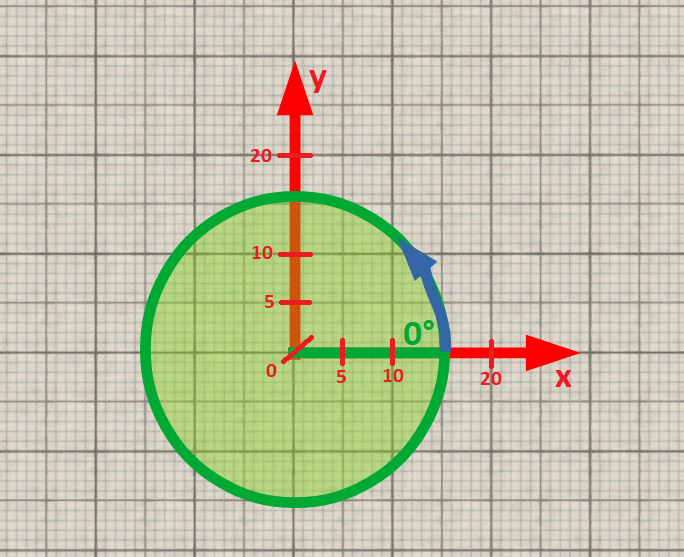
\includegraphics[width=.6\linewidth]{pictures/2019-08-12_envCooSystem.png} % chktex 8
    \medskip
    \caption{%
        Environment coordinate system --- Visualizes the theoretical view on an environment.
        For purpose of illustration the underlying grid shows squares which group 5 by 5 cells where each cell has an edge length of \SI{1}{\metre}.
        This grid is not visible during a simulation.
    }\label{fig:envCooSystem}
\end{figure}
A \gls{dbe} specifies environment elements \ie{} roads and obstacles.
A road has a course, a number of left and right lanes and optionally has road markings and a name.
The course is a sequence of tuples where each tuple contains a road center point and the current width of the road at that point.
This representation allows to easily calculate the distance of an \gls{av} to the road center and to determine the direction of lanes.
The number of left and right lanes influences the types of road markings in case a road has markings.
Right lanes go in the same direction as the sequence of the road center points.
Left lanes go in the opposite direction.
In order to define basic static surroundings like buildings the formalization allows obstacles of type cube, cylinder, cone and bump.
Obstacles can not be moved by participants, do not deform and are unbreakable.
\Cref{fig:exampleEnvironmentVis} depicts simple examples of generated environment elements.
\begin{figure}
    \centering
    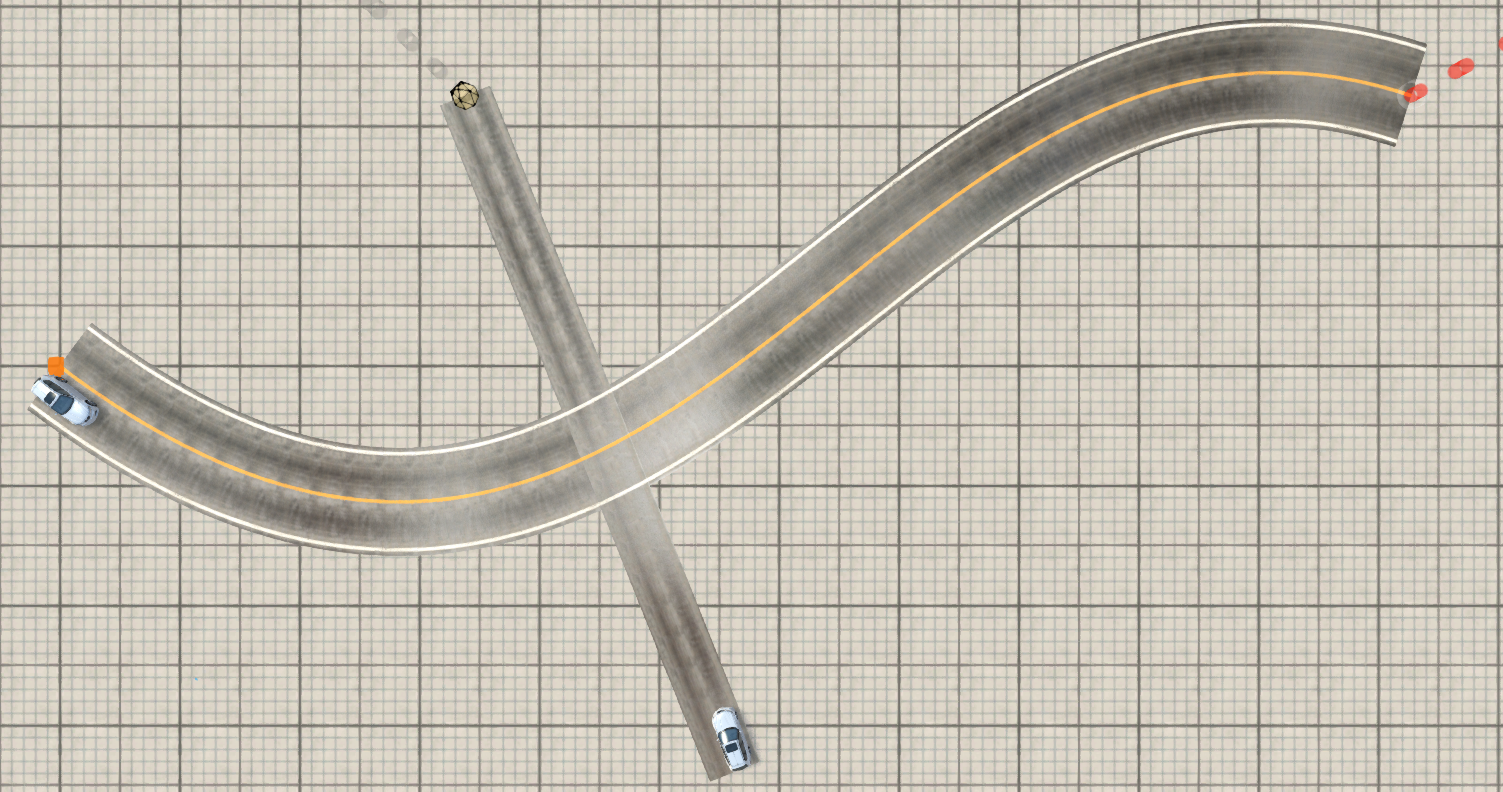
\includegraphics[width=\linewidth]{pictures/2019-08-15_simpleLanes.png} % chktex 8
    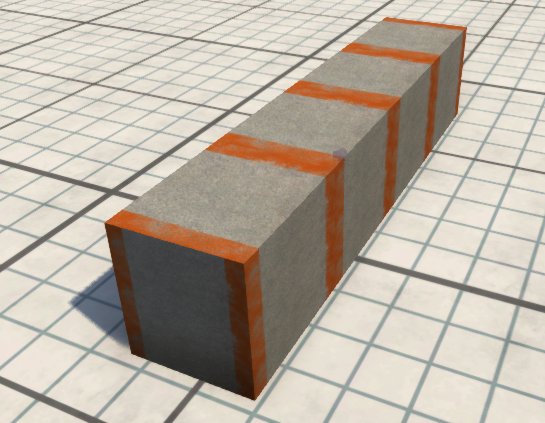
\includegraphics[height=70px]{pictures/cube.png}
    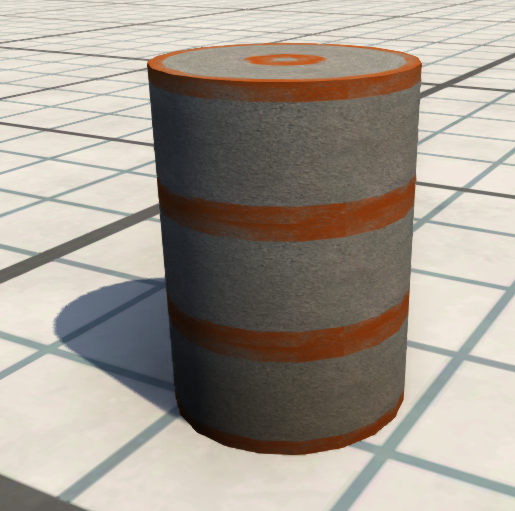
\includegraphics[height=70px]{pictures/cylinder.png}
    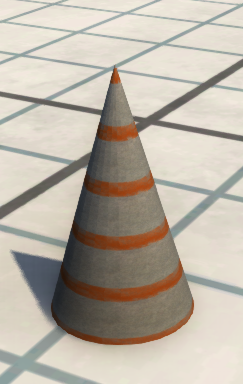
\includegraphics[height=70px]{pictures/cone.png}
    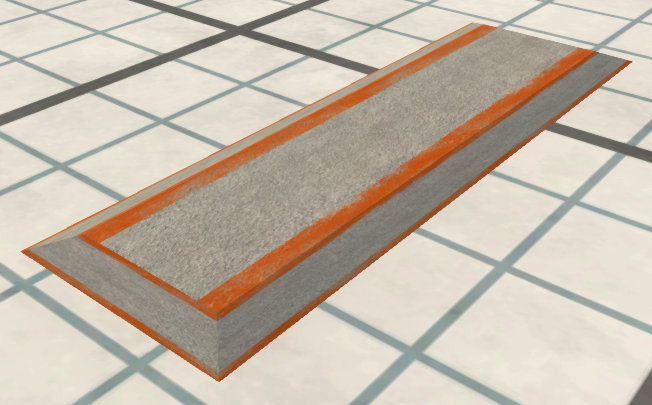
\includegraphics[height=70px]{pictures/bump.png}
    \medskip
    \caption{%
        Visualization of example environment elements --- Shows generated static environment elements including two roads and multiple obstacles.
        For purpose of illustration the underlying grid shows squares which group 5 by 5 cells where each cell has an edge length of \SI{1}{\metre}.
        This grid is not visible during a simulation.
        \Cref{fig:exampleEnvironment,fig:exampleObstacleDefinitions} in the appendix show the declarations to generate these environment elements.
    }\label{fig:exampleEnvironmentVis}
\end{figure}
\subsubsection{Formalization of Criteria}
The test criteria divide in precondition, success and fail criteria.
Typically a test is considered as successful if it ends without triggering the fail criterion.
In the context of testing \glspl{av} this may not be always true since the tests are very complex and there are cases where an \gls{av} does not succeed but a tester does not want the test to be marked as failed.
A very common example is a test like \enquote{The \gls{av} is successful if it reaches a certain position and fails if it takes any damage or goes off-road}.
If the \gls{av} under test does not move at all it does not pass the test.
That the \gls{av} does currently not move does not imply that is not going to move at some point in the future.
Hence it can not be concluded that the test failed.
To describe such results \drivebuild{} uses a three-valued logics.
The most basic one is the Kleene and Priest logics~\cite{kleeneLogics} which declares besides \iltrue{} and \ilfalse{} also the value \ilunknown{}.
Since the third value \ilunknown{} is neutral to all connectives it can express that a criterion could not be determined or is currently not considered without influencing the outcome of the overall criterion.
The definition of test criteria follows the concept of temporal logic and thus defines \glspl{sc}, \glspl{vc} and connectives (\iland{}, \ilor{} and \ilnot{}) which can be nested as \cref{fig:nesting} visualizes.
\begin{figure}
    \centering
    \begin{tikzpicture}[%
        ->,
        >=stealth
    ]
    \node (evaluation) {\itshape criterion};
    \node[above=of evaluation] (start) {};
    \node[below=of evaluation] (criterion) {\itshape evaluation};
    \node[left=of criterion] (connective) {\itshape connective};
    \node[below=of connective] (and) {and};
    \node[right=of and] (or) {or};
    \node[left=of and] (not) {not};
    \node[below=of criterion] (sc) {\glstext{sc}};
    \node[right=of sc] (vc) {\glstext{vc}};

    \path
        (start) edge (evaluation)
        (evaluation) edge (criterion)
        (evaluation) edge[bend left]  (connective)
        (connective) edge[bend left] (evaluation)
        (criterion) edge (sc)
        (criterion) edge (vc)
        (vc) edge[bend right] (evaluation)
        (connective) edge (not)
        (connective) edge (and)
        (connective) edge (or);
\end{tikzpicture}


    \medskip
    \caption{%
        Nesting of a criterion --- Shows the allowed nesting structure for \glspl{sc}, \glspl{vc} and connectives to define a criterion. Italic types are abstract.
    }\label{fig:nesting}
\end{figure}
\Glspl{sc} as well as \glspl{vc} evaluate the current state of the simulation or an \gls{av} and determine whether it fulfills a certain condition.
\Glspl{sc} yield in case the criterion can be evaluated either \iltrue{} or \ilfalse{}.
Otherwise it returns \ilunknown{}.
\Glspl{vc} restrict whether the inner criterion has to be considered in the evaluation of the parent criterion.
If the condition of the \gls{vc} is \iltrue{} the inner criterion is evaluated and the \gls{vc} returns its result.
Otherwise the \gls{vc} returns \ilunknown{}.
The introduction of \glspl{vc} allows to evaluate different criteria under different circumstances.
This allows to enable or disable criteria under certain circumstances.
\Eg{} define a fail criterion like \enquote{While \gls{av} \(A\) drives on road \(R\) it must not exceed a speed limit of \(S\)}.
In this case the speed of \(A\) should only be evaluated as long as \(A\) drives on \(R\) and return ideally either \iltrue{} or \ilfalse{}.
If \(A\) is not on \(R\) \ilunknown{} shall be returned to ignore the criterion.
Another use case for \glspl{vc} may be to define that an \gls{av} is allowed to leave the road as long as it is in a certain area \eg{} to avoid an obstacle or another participant that blocks the road in this area.
\Cref{tab:criteriaTypes} lists all supported kinds of criteria and whether they can be used as \gls{vc} or \gls{sc}.
\begin{table}
    \centering
    \caption{%
        Test criteria --- Lists all supported test criteria, describes their purpose and characterizes whether these can be used for \glspl{vc} or \glspl{sc}.
    }\label{tab:criteriaTypes}
    \medskip
    %!TEX root = ../thesis.tex
\begin{tabularx}{\linewidth}{l X c c}
    \toprule
    \bfseries Type & \bfseries Description & \bfseries \glstext{vc} & \bfseries \glstext{sc} \\
    \midrule
    position & Checks whether an \gls{av} is at a certain position or within a certain radius of it & \checkmark{} & \checkmark{} \\
    area & Checks whether an \gls{av} is within a certain area & \checkmark{} & \checkmark{} \\
    lane & Checks whether an \gls{av} drives on a certain lane or off-road & \checkmark{} & \checkmark{} \\
    speed & Checks whether the speed of an \gls{av} is below a given velocity & \checkmark{} & \checkmark{} \\
    damage & Checks whether an \glspl{av} is damaged & \checkmark{} & \checkmark{} \\
    time & Checks whether the simulation is currently within a certain interval of ticks & \checkmark{} & \ding{53} \\
    distance & Checks whether the distance between two \glspl{av} or between an \gls{av} and the center of the lane driving on is smaller than a given distance & \checkmark{} & \checkmark{} \\
    \glstext{ttc} & Checks whether the \glsfirst{ttc} of an \gls{av} and another participant or obstacle is smaller than a given value & \checkmark{} & \ding{53} \\
    \bottomrule
\end{tabularx}


\end{table}
\Cref{fig:exampleCriteria} in the appendix shows example definitions for all of them.
Using the mechanism which \cref{sec:runtimeVerification} explains a tester can introduce additional client side criteria.
\subsubsection{Formalization of Participants}
The declaration of a participant specifies always a car model and an initial state.
The chosen model fixes the shape and the physics of the participant.
The set of available models is a predefined set which comes with \beamng{}.
The initial state specifies the initial position and the initial orientation of a participant.
If a participant is an \gls{av} the underlying \gls{ai} and its \glspl{adas} require data to operate.
The formalization allows to declaratively specify this data which a simulation has to collect and provide.\\
Resulting from the metrics which \glspl{adas} require in \cref{tab:reqData} and the available test criteria in \cref{tab:criteriaTypes} I determined multiple types of request data (see \cref{tab:aiData}) which a formalization can declare and which a simulation can provide.
\begin{table}
    \caption{%
        Available request data --- Lists all types of request data which an \gls{ai} that registered at a simulation can possibly request and whether it can be considered as sensor data.
    }\label{tab:aiData}
    \medskip
    %!TEX root = ../thesis.tex
\begin{tabularx}{\linewidth}{l X c}
    \toprule
    \bfseries Type          & \bfseries Description                                                             & \bfseries Sensor Data \\
    \midrule
    position                & Absolute position of an \gls{av}                                                  & \ding{53}             \\
    speed                   & Absolute speed of an \gls{av}                                                     & \checkmark{}          \\
    steering angle          & Current steering angle of the steering wheel                                      & \checkmark{}          \\
    \Glstext{lidar}         & Distance data provided by a \gls{lidar} sensor                                    & \checkmark{}          \\
    camera                  & Camera images either colored, annotated or with depth information                 & \checkmark{}          \\
    damage                  & Detects whether an \gls{av} is damaged                                            & \checkmark{}          \\
    distance to road center & Distance to the center of the nearest road                                        & \ding{53}             \\
    heading angle           & Angle between the orientation of a participant and the center of the nearest road & \ding{53}             \\
    bounding box            & The bounding box of a participant                                                 & \ding{53}             \\
    road edges              & Sequences of points for the right and left edge of a road                         & \ding{53}             \\
    \bottomrule
\end{tabularx}


\end{table}
It also shows which of the request data can be considered as sensor data and thus marks on which request data an \gls{ai} should rely in order to be realistic.
The other types of request data can be used to collect training data, to compare the computed results of an \gls{ai} to a ground truth or to implement additional client side criteria before or after the computations which an \gls{ai} does.\\
In case the participant is not autonomous the declaration may specify a movement.
A movement is a sequence of waypoints which a participant has to follow.
A waypoint is a position at which the behavior of a participant may change.
It also has a tolerance value which avoids that a participant has to precisely reach a position and allows to pass by in a certain distance.
A waypoint optionally defines a speed limit or a target speed which a participant has to obey until it reaches the next waypoint that specifies another value for them.
Both the initial state and all waypoints have an attribute which specifying the current movement mode of a participant.
The movement mode is one of \mmmanual{}, \mmautonomous{} and \mmtraining{}.
If the current movement mode of a participant is \mmmanual{} the car heads straight to the next waypoint and the target speed as well as the speed limit apply.
If the movement mode is \mmautonomous{} the simulation requests the \gls{ai} that registered for controlling the \gls{av} frequently and provides it with data.
If the movement mode is set to \mmtraining{} the \gls{av} acts the same way it does in \mmmanual{} but the simulation requests the connected \gls{ai} like in \mmautonomous{}.
In contrast to \mmautonomous{} the \gls{ai} can not control the \gls{av}.
However, the \gls{ai} can still control the simulation.
This mode is geared towards collecting training data for \glspl{ai}.
The strategy to allow to change movement modes at each waypoint enables to mix sections where a participant is forced to follow a path, where an \gls{ai} has to control it or where to collect data.
\Cref{fig:exampleParticipant,fig:exampleAIDataRequests} in the appendix show example definitions of participants as well as example declarations of many request data.
\Cref{fig:exampleParticipantVis} shows the corresponding graphical representation of the participant and its movement.
\begin{figure}
    \centering
    \includegraphics[width=.9\linewidth]{pictures/2019-08-15_ParticipantMovements.png} % chktex 8
    \medskip
    \caption{%
        Visualization of example participants --- Shows participants and their movements generated from the declarations in \cref{fig:exampleParticipant} in the appendix.
        The green line marks the parts of a path where a participant is in \mmmanual{} mode and has to follow the waypoints.
        The red stripe marks the area an \gls{av} in \mmautonomous{} mode is expected to follow but not forced to.
        In this case the participants do not change their movement mode during the simulation.
    }\label{fig:exampleParticipantVis}
\end{figure}

\subsection{Test Life Cycle}\label{sec:testCycle}
\Cref{fig:testCycle} shows all phases of the test life cycle and groups them into the four main steps \textcolor{blue}{input validation}, \textcolor{magenta}{extraction}, \textcolor{cyan}{transformation} and \textcolor{red}{execution}.\\
\begin{figure}
    \centering
    \begin{tikzpicture}[%
        ->,
        >=stealth
    ]
    \node at (-3.2,0) (Tester) {Test};
    \node at (-1,0) (Validation) {\textcolor{blue}{Input Validation}};
    \node at (2,0.5) (Environment) {\textcolor{magenta}{Environment}};
    \node at (2,1.5) (Participants) {\textcolor{magenta}{Participants}};
    \node at (5,1.5) (Movements) {\textcolor{magenta}{Movements}};
    \node at (2,-0.5) (Criteria) {\textcolor{magenta}{Criteria}};
    \node at (5,-0.5) (Transform) {\textcolor{cyan}{Transformation}};
    \node at (5,0.5) (Generation) {\textcolor{cyan}{Generation}};
    \node at (8,1.5) (Simulation) {\textcolor{red}{Simulation}};
    \node at (8,-0.5) (Verification) {\textcolor{red}{Verification}};
    \node at (10.3,-0.5) (Results) {Results};
    \path
        (Tester) edge (Validation)
        (Validation) edge (Environment)
        (Environment) edge (Generation)
        (Generation) edge (Simulation)
        (Validation) edge (Participants)
        (Participants) edge (Movements)
        (Movements) edge (Simulation)
        (Participants) edge (Generation)
        (Validation) edge (Criteria)
        (Criteria) edge (Transform)
        (Transform) edge (Verification)
        (Verification) edge[bend left] (Simulation)
        (Simulation) edge[bend left] (Verification)
        (Verification) edge (Results);
\end{tikzpicture}

    \medskip
    \caption{%
        Test life cycle --- Visualizes the four main steps of processing a formalized test.
        The input validation step is \textcolor{blue}{blue}, the extraction step is \textcolor{magenta}{magenta}, the transformation step is \textcolor{cyan}{cyan} and the execution step is \textcolor{red}{red}.
    }\label{fig:testCycle}
\end{figure}
The input validation checks whether the test case is broken or malformed and validates it against the \gls{xsd} which enforces the structure of the formalized test case.
If the test case is valid the process extracts the environment description, the test criteria and the participants.
It passes the information about roads, obstacles and participants in the environment to the generator which creates representations that are compatible with the underlying simulator.
The representation of the movements of the participants are passed directly to \beamng{} which applies them sequentially to the appropriate participants as soon as the simulation started.
The transformation step creates Kleene and Priest logics expressions which represent the defined test criteria.
The verification process uses these expressions to verify the criteria during the simulation.
Then \beamng{} starts the execution of the test and sets up the runtime verification process (see \cref{sec:runtimeVerification}).
As soon as the runtime verification is able to determine whether the test succeeded or failed it stops the simulation and returns its test result.

\subsection{Runtime Verification}\label{sec:runtimeVerification}
The runtime verification cycle applies synchronous simulation (see \cref{sec:background}) and \cref{fig:runtimeVerification} depicts its five phases.
\begin{figure}
    \centering
    \smartdiagram[flow diagram:horizontal]{%
        Verify criteria, Request \glspl{ai}, Control, Step, Pause
    }
    \medskip
    \caption{%
        Runtime verification cycle --- Depicts the main phases which implement the runtime verification and applies the synchronous simulation.
    }\label{fig:runtimeVerification}
\end{figure}
The first phase checks whether the current state of the simulation yields a test result.
Therefore it uses a decision tree where the leaves represent test results and the inner nodes represent the evaluation of the precondition, the fail and the success criterion.
The inner nodes work with lazy evaluation and \cref{fig:verificationDecision} shows the complete tree.
\begin{figure}
    \centering
    \begin{tikzpicture}[%
    ->,
    >=stealth
]
    \node (start) {};
    \node[right=of start] (preconds) {Precondition};
    % \node[below=of preconds] (skipped) {\underline{\vsmskipped{}}}; % FIXME Does not work
    \node[below=of preconds] (skipped) {\underline{\code{SKIPPED}}};
    \node[right=of preconds] (fail) {Fail criterion};
    % \node[below=of fail] (tcFail) {\underline{\vsmfailed{}}}; % FIXME Does not work
    \node[below=of fail] (tcFail) {\underline{\code{FAILED}}};
    \node[right=of fail] (success) {Success criterion};
    % \node[below=of success] (tcSuccess) {\underline{\vsmsucceeded{}}}; % FIXME Does not work
    \node[below=of success] (tcSuccess) {\underline{\code{SUCCEEDED}}};
    % \node[right=of success] (undetermined) {\underline{\vsmunknown{}}}; % FIXME Does not work
    \node[right=of success] (undetermined) {\underline{\code{UNKNOWN}}};

    \path (start) edge (preconds);
    \draw[red] (preconds) edge (skipped);
    \draw[green] (preconds) edge[bend left] (fail);
    \draw[blue] (preconds) edge[bend right] (fail);
    \draw[green] (fail) edge (tcFail);
    \draw[red] (fail) edge[bend left] (success);
    \draw[blue] (fail) edge[bend right] (success);
    \draw[green] (success) edge (tcSuccess);
    \draw[red] (success) edge[bend left] (undetermined);
    \draw[blue] (success) edge[bend right] (undetermined);
\end{tikzpicture}

    \medskip
    \caption{%
        Test result decision tree --- Visualizes the structure of the decision tree which determines the current test result.
        Underlined nodes are leaves and represent test results.
        The inner nodes represent the criteria of the test.
        Arrows describe the transitions from node to node which depends on whether a criterion evaluated to \colorbox{green!50}{true}, \colorbox{red!50}{false} or \colorbox{blue!40}{unknown}.
    }\label{fig:verificationDecision}
\end{figure}
If the decision tree yields either \trskipped{}, \trfailed{} or \trsucceeded{} the simulation stops and returns the current test result as final test result.
In this case all \glspl{ai} which are registered at the simulation are notified about the end of the simulation as well.
If the current test result is \trunknown{} the runtime verification cycle continues with the next phase.
The second phase implements the exchange of data with \glspl{ai}.
Therefore it updates all data of any sensor and all properties of any participant which were declared in the \gls{dbc} or are required to evaluate the test criteria.
The phase also searches for all \glspl{av} that are in movement mode \mmautonomous{} or \mmtraining{}, notifies the \glspl{ai} which registered for these \glspl{av} about the availability of new data and waits for them to send commands which control the \glspl{av} or the simulation.
\Cref{fig:aiSimProtocol} depicts the three-way protocol which the communication uses.
\begin{figure}
    \centering
    \documentclass{standalone}

\usepackage[acronym,automake,toc]{glossaries}
\usepackage{pgf-umlsd}

\makeglossaries%
\loadglsentries{../acronyms.tex}

\begin{document}

\begin{sequencediagram}
    \newthread{sim}{:Simulation}
    \newinst{dummy}{Dummy placeholder}
    \newthread{ai}{:\glstext{ai}}
    \begin{call}{ai}{Wait for request}{sim}{Send alive message}
        \begin{callself}{sim}{Simulate}{}
        \end{callself}
    \end{call}
    \begin{call}{ai}{Request simulation data}{sim}{Send simulation data}
    \end{call}
    \begin{callself}{ai}{Calculate control commands}{}
    \end{callself}
    \begin{call}{ai}{Control simulation}{sim}{Send alive message}
    \end{call}
\end{sequencediagram}


\end{document}

    \medskip
    \caption{%
        Communication between a simulation and an \glstext{ai} --- Visualizes the messages of the three-way protocol sent for exchanging data between a simulation and an \glstext{ai}.
    }\label{fig:aiSimProtocol}
\end{figure}
The first message registers an \gls{ai} at a certain simulation for a certain \gls{av} and blocks until the simulation notifies it about new data.
Its response contains the current state of the simulation which is either \ssrunning{}, \ssfinished{}, \sscanceled{} or \sstimeout{}.
The state of the simulation may be \ssunknown{} which is only the case if the simulation could not be found.
These states allow an \gls{ai} to determine whether a simulation exists and whether it still runs or already stopped.
They also allow to determine the reason why the simulation stopped.
If the state of the simulation is \ssrunning{} the \gls{ai} requests sensor data or properties of its associated \gls{av} for which it needs to calculate control commands.
A control command for an \gls{av} is a tuple which contains values for acceleration, brake intensity and steering angle.
A command to control a simulation contains only the test result which has to be enforced.
The opportunity to control a simulation allows an \gls{ai} to eventually stop the simulation after the evaluation of client side criteria.\\
The control phase applies the commands which the \glspl{ai} sent.
In case one of them enforces a test result the simulation stops.
Otherwise the phase applies all control commands of the \glspl{ai} to their associated \gls{av} the runtime verification continues with the next phase.
In this phase \beamng{} calculates the changes to the simulation for the next number of ticks as defined by the \gls{ai} frequency, applies them and pauses the simulation again.
Then the runtime verification cycle starts from the beginning.

\subsection{Cluster Architecture}
The architecture of \drivebuild{} uses a master slave model.
The slave components are \glspl{simnode} that manage running simulations and runtime verification processes.
The master component is the \gls{mainapp}.
It organizes all \glspl{simnode} and offers the entry point for all clients and \glspl{ai}.\\
\Cref{fig:systemArch} depicts all logical components of \drivebuild{}, their data flow and how they are grouped to modules that can be distributed over a cluster.
\begin{figure}
    \centering
    %!TEX root = ../thesis.tex
\begin{tikzpicture}[%
    ->,
    >=stealth
]
\tikzset{%
    node distance=2.5
}
\node (tester) {Tester};
\node[below=of tester] (tcmanager) {\Glstext{tcmanager}};
\node[right=of tester] (ai) {\Glstext{ai}};
\node[below=of ai] (communicator) {{{\scshape Communicator}}};
\node[below=4 of tcmanager] (simcontroller) {\Glstext{simcontroller}};
\node[left=1.3 of simcontroller] (transformer) {{{\scshape Transformer}}};
\node[above=.1 of transformer] (fitExtension) {};
\node[left=1.9 of transformer] (generator) {{{\scshape Generator}}};
\node[above=1.8 of transformer] (dbms) {\Glstext{dbms}};
\node[above=1.7 of dbms] (stats) {\Glstext{statsmanager}};
\node[above=of stats] (researcher) {Researcher};
\node[below=of transformer] (kptransformer) {\Glstext{kptransformer}};
\node[below=of simcontroller] (verificator) {\mltn{Runtime Verification\\Process 1\ldots N}};
\node[right=0.5 of verificator] (simulatorA) {Simulation 1\ldots N};

% Client backgrounds
\node[zlayer=back,fill=clusterClient,fit={(researcher)}] {};
\node[zlayer=back,fill=clusterClient,fit={(tester)}] {};
\node[zlayer=back,fill=clusterClient,fit={(ai)}] {};
% Stack 1
\node[below right=-0.5mm and 0.5mm of ai.south west] (aiStackA) {};
\node[below right=-0.5mm and -0.5mm of ai.south east] (aiStackB) {};
\node[below right=0.5mm and -0.5mm of ai.north east] (aiStackC) {};
\node[zlayer=back,fill={rgb,255:red,112;green,112;blue,255},fit={(aiStackA)(aiStackB)(aiStackC)},inner sep=0] (aiStackA) {};
% Stack 2
\node[below right=-1.5mm and 0.5mm of aiStackA.south west] (aiStackAA) {};
\node[below right=-1.5mm and -1.5mm of aiStackA.south east] (aiStackBB) {};
\node[below right=0.5mm and -1.5mm of aiStackA.north east] (aiStackCC) {};
\node[zlayer=back,fill={rgb,255:red,0;green,0;blue,255},fit={(aiStackAA)(aiStackBB)(aiStackCC)},inner sep=0] {};
% Redraw previous stacks in reverse order
\node[zlayer=back,fill={rgb,255:red,112;green,112;blue,255},fit={(aiStackA)(aiStackB)(aiStackC)},inner sep=0] (aiStackA) {};
\node[zlayer=back,fill=clusterClient,fit={(ai)}] {};

% SimNode backgrounds
\node[zlayer=back,fill=clusterSimNode,fit={(simulatorA)(kptransformer)(verificator)(generator)(fitExtension)}] (server) {};
% Stack 1
\node[below right=0mm and 3mm of server.south west] (simNodeStackA) {};
\node[below right=0mm and 0mm of server.south east] (simNodeStackB) {};
\node[below right=3mm and 0mm of server.north east] (simNodeStackC) {};
\node[zlayer=back,fill={rgb,255:red,112;green,255;blue,112},fit={(simNodeStackA)(simNodeStackB)(simNodeStackC)},inner sep=0] (stackA) {};
% Stack 2
\node[below right=0mm and 3mm of stackA.south west] (simNodeStackAA) {};
\node[below right=0mm and 0mm of stackA.south east] (simNodeStackBB) {};
\node[below right=3mm and 0mm of stackA.north east] (simNodeStackCC) {};
\node[zlayer=back,fill={rgb,255:red,0;green,220;blue,0},fit={(simNodeStackAA)(simNodeStackBB)(simNodeStackCC)},inner sep=0] {};
% Redraw previous stacks in reverse order
\node[zlayer=back,fill={rgb,255:red,112;green,255;blue,112},fit={(simNodeStackA)(simNodeStackB)(simNodeStackC)},inner sep=0] (stackA) {};
\node[zlayer=back,fill=clusterSimNode,fit={(simulatorA)(kptransformer)(verificator)(generator)(fitExtension)}] (serverRedraw) {};

% MainApp background
\node[zlayer=back,fill=clusterMicroService,fit={(tcmanager)(communicator)(stats)}] (microserviceA) {};

% DBMS background
\node[zlayer=back,fill=clusterDbms,fit={(dbms)}] (dbmsComponent) {};

\path
    (tester) edge node[above]{SimulationID} node[below]{VehicleID} (ai)
    (tester) edge[bend right] node[rotate=90,above]{Test Case} (tcmanager)
    (dbms) edge (stats)
    (stats) edge (researcher)
    (researcher) edge (stats)
    (simcontroller) edge (dbms)
    (simcontroller) edge (transformer)
    (transformer) edge (simcontroller)
    (tcmanager) edge[bend right] node[rotate=-90,above] {SimulationID} (tester)
    (transformer) edge node[rotate=90,above]{Criteria} (kptransformer)
    (kptransformer) edge (transformer)
    (transformer) edge node[above] {Lanes, \Glspl{av},} (generator)
    (transformer) edge node[below] {Obstacles} (generator)
    (generator) edge (transformer)
    (tcmanager) edge[bend right] node[rotate=90,above] {Test Case} (simcontroller)
    (simcontroller) edge[bend right] node[rotate=-90,above] {SimulationID} (tcmanager)
    (simcontroller) edge node[rotate=90,above] {Runtime} (verificator)
    (verificator) edge node[rotate=90,below] {Verification} (simcontroller)
    (simcontroller.south east) edge (simulatorA)
    (simulatorA) edge (simcontroller.south east)
    (simcontroller.north east) edge (communicator)
    (communicator) edge (simcontroller.north east)
    (communicator) edge (ai)
    (ai) edge (communicator);
\end{tikzpicture}

    \medskip
    \caption{%
        Cluster architecture --- Visualizes all logical components of \drivebuild{} and the data flow between them.
        It also groups the components into the modules \colorbox{clusterClient}{client}, \colorbox{clusterMicroService}{\glstext{mainapp}}, \colorbox{clusterDbms}{\glstext{dbms}} and \colorbox{clusterSimNode}{\glstext{simnode}}.
    }\label{fig:systemArch}
\end{figure}
The architecture considers three different types of clients \ie{} testers who execute tests, \glspl{ai} that control \glspl{av} in simulations and researchers who access collected data.
A tester submits test cases to the \gls{tcmanager} which selects a \gls{simnode} based on the load distribution strategy.
For load distribution the \gls{tcmanager} selects the \gls{simnode} where currently the least number of simulations run and passes each test to a new \gls{simcontroller} instance at that \gls{simnode}.
The \gls{simcontroller} creates and manages the \beamng{} instance which executes the test and starts a runtime verification process that \cref{sec:runtimeVerification} describes in more detail.
It also provides methods to request and monitor the current state of a test execution to the \gls{tcmanager}.
The \gls{simcontroller} passes the test to the \transformer{} which checks its validity, extracts static and dynamic information about the environment and the participants and generates a semantic representation.
The \transformer{} also creates temporal logic expressions from the defined criteria such that these can be easily evaluated during the simulation by providing only the current state of the simulation as input.
The \gls{simcontroller} uses the semantic representation to generate a \beamng{} scenario and executes it.
When a simulation ends the \gls{simcontroller} stores the initial \gls{dbe} and \gls{dbc} along with its test result and other statistics which the evaluation needs in the database (see \cref{sec:evaluation}).
The \communicator{} handles the exchange of messages between a \gls{simcontroller} and \glspl{ai} during a simulation and allows to collect training data.
Therefore it uses the protocol which \cref{fig:aiSimProtocol} visualizes.
The \gls{statsmanager} grants access to the data which \glspl{simcontroller} store in the database and thus enables researchers to investigate and analyze collected data about test cases, their executions and their test results.\\
\Cref{fig:distributeNodes} visualizes how the modules of \drivebuild{} distribute over a cluster and how they communicate with each other and the client.
\begin{figure}
    \centering
    \begin{tikzpicture}[%
        ->,
        >=stealth
    ]
    \node (client) {
\includegraphics[width=.125\linewidth]{pictures/computer_client.png}};
    \node[above=.7 of client] (ai1) {
\includegraphics[width=.125\linewidth]{pictures/ai.png}};
    \node[below=.7 of client] (ai2) {
\includegraphics[width=.125\linewidth]{pictures/ai.png}};
    \node[right=1.5 of client] (microService) {
\includegraphics[width=.125\linewidth]{pictures/virtualMachine_microService.png}};
    \node[right=1.5 of microService] (windows2) {
\includegraphics[width=.0625\linewidth]{pictures/virtualMachine_windows.png}};
    \node[above=0.5 of windows2] (windows1) {
\includegraphics[width=.0625\linewidth]{pictures/virtualMachine_windows.png}};
    \node[below=0.25 of windows2] (dots) {\vdots};
    \node[below=0.25 of dots] (windows3) {
\includegraphics[width=.0625\linewidth]{pictures/virtualMachine_windows.png}};
    \node[right=1.5 of windows2] (dbms) {
\includegraphics[width=.0625\linewidth]{pictures/dbms.png}};

    \draw
        (client) edge (microService)
        (microService) edge (client)
        (ai1) edge (microService)
        (microService) edge (ai1)
        (ai2) edge (microService)
        (microService) edge (ai2)
        (microService) edge (windows1)
        (windows1) edge (microService)
        (microService) edge (windows2)
        (windows2) edge (microService)
        (microService) edge (windows3)
        (windows3) edge (microService)
        (dbms) edge (windows1)
        (windows1) edge (dbms)
        (dbms) edge (windows2)
        (windows2) edge (dbms)
        (dbms) edge (windows3)
        (windows3) edge (dbms)
        (microService) edge[bend left=70] (dbms) % FIXME These two edges needed?
        (dbms) edge[bend right=70] (microService);

    % Labels
    \node[below=.2 of ai2] (clientLabel) {\colorbox{clusterClient}{Client}};
    \node[right=1.8 of clientLabel] (mainAppLabel) {\colorbox{clusterMicroService}{\Glstext{mainapp}}};
    \node[right=1.2 of mainAppLabel] (simNodeLabel) {\colorbox{clusterSimNode}{\Glstext{simnode}}};
    \node[right=.9 of simNodeLabel] (dbmsLabel) {\colorbox{clusterDbms}{\Glstext{dbms}}};

    % Cluster box
    \node[draw,fit={(microService)(dbms)(windows1)(windows3)},inner sep=3mm,line width=0.5mm] (clusterBox) {};
    \node[above=.1 of clusterBox.north east, anchor=south east] {Cluster};
\end{tikzpicture}

    \medskip
    \caption{%
        Distribution of modules over a cluster --- Visualizes how the modules of \drivebuild{} (see \cref{fig:systemArch}) distribute over multiple nodes in a cluster and how they communicate with each other and the client.
    }\label{fig:distributeNodes}
\end{figure}
A client uploads formalized test cases to the \gls{mainapp} which distributes the test cases amongst a number of registered \glspl{simnode}.
Further a client starts instances of \glspl{ai} which also connect to the \gls{mainapp} in order to interact with the \glspl{av} which the uploaded test cases declare.
Conceptually, the \gls{mainapp} as well as the \glspl{simnode} exchange data with the database and may run in \glspl{vm}.


    %!TEX root = ../thesis.tex
\section{Implementation}\label{sec:implementation}
\subsection{Used Tools, Frameworks and Libraries}
\Cref{tab:usedTools} lists all tools, frameworks and libraries \drivebuild{} uses, characterizes them by whether the \gls{mainapp}, a \gls{simnode} or a client implementation requires them and shows whether they are just a dependency of another element.
This section describes the most essential tools, frameworks and libraries in detail and why they were chosen.\\
\beamng{}~\cite{beamNG} is a racing game that is free to use for research purposes.
It comes with a highly accurate physics engine and thus it is interesting for research as well.
Most simulators have a top down approach where the physics of a vehicle are specified as a whole and the properties and behavior of all components of the car derive from it.
In contrast \beamng{} uses a bottom up approach where each tire, car suspension, the chassis, the engine, every cross beam, \etc{} has its own physics.
A vehicle is a collection of these components which are connected by beams and thus the physics the vehicle results from the physics of its components.\\
\beamngpy{}~\cite{beamngpy} is a Python interface for \beamng{}.
It allows to programmatically create scenarios, attach many kinds of sensors to vehicles, collect data and handle simulations and participants during simulations.
\beamngpy{} can also access the pixel perfect annotation mode in which a camera returns images that mark on the image where buildings, roads, other participants \etc{} are.
This can be used to gather training data for \glspl{ai}.
Since \beamngpy{} is not able to handle parallel requests to the same \beamng{} instance \drivebuild{} wraps \beamngpy{} and introduces locks to implement basic thread safety.\\
\dill{} is a library which can serialize Python objects and extends the capabilities of the \pickle{} module that ships with Python.
\glspl{simnode} have to serialize parameters when a process starts a new thread \eg{} start a new \beamng{} instance and requires arguments.\\
\flask{}~\cite{flask} is a framework to create micro service based webservices.
It is well known, reliable and uses annotations to map addresses with functions and parameters which makes it easy to use.\\
\lxml{}~\cite{lxml} is a library for handling \gls{html} and \gls{xml} files.
It provides methods to parse and validate \gls{xml} files against \glspl{xsd} and to traverse them with XPath expressions.
\lxml{} is basically just a Python interface to the well known, reliable and very fast C libraries libxml2~\cite{libxml2} and libxslt~\cite{libxslt}.\\
\Gls{protobuf}~\cite{protobuf} is a tool to specify and handle messages in a more type safe way than basic byte streams offer.
Therefore it provides a language to define the structure of messages and the data types of their attributes.
\Gls{protobuf} is able to cross compile these definitions to appropriate representations in a set of well known programming languages including Python, Java, C++ and Haskell.
The compilation process introduces additional methods to serialize and parse messages and to check the existence of attributes in messages.\\
\winpython{}~\cite{winpython} is a Python distribution that ships with a set of Python packages for which the installation on Windows is complex or error prone.
This includes especially packages like \scipy{} which \drivebuild{} requires.
\subsection{Communication}\label{subsec:communication}
Both the content of \gls{http} requests as well as of socket messages is serialized byte data which represents \glspl{pmessage}.
The communication uses the generated serialization methods of \Gls{protobuf} to convert \glspl{pmessage} from and to byte data.
\Cref{fig:simpleMessages} lists all simple and \cref{fig:complexMessages} visualizes all complex \glspl{pmessage} which the communication can handle as well as their structure.
\begin{figure}
    \centering
    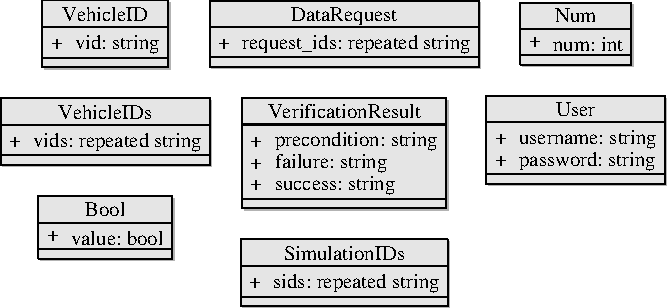
\includegraphics[width=\textwidth, height=.95\textheight, keepaspectratio]{diagrams/messagesTypeGraph-1.pdf}
    \medskip
    \caption{%
        Simple \glspl{pmessage} --- Shows all basic \glspl{pmessage} which do neither contain nor are nested in other \glspl{pmessage}.
        It also lists their attributes with the appropriate type.
    }\label{fig:simpleMessages}
\end{figure}
\begin{figure}
    \centering
    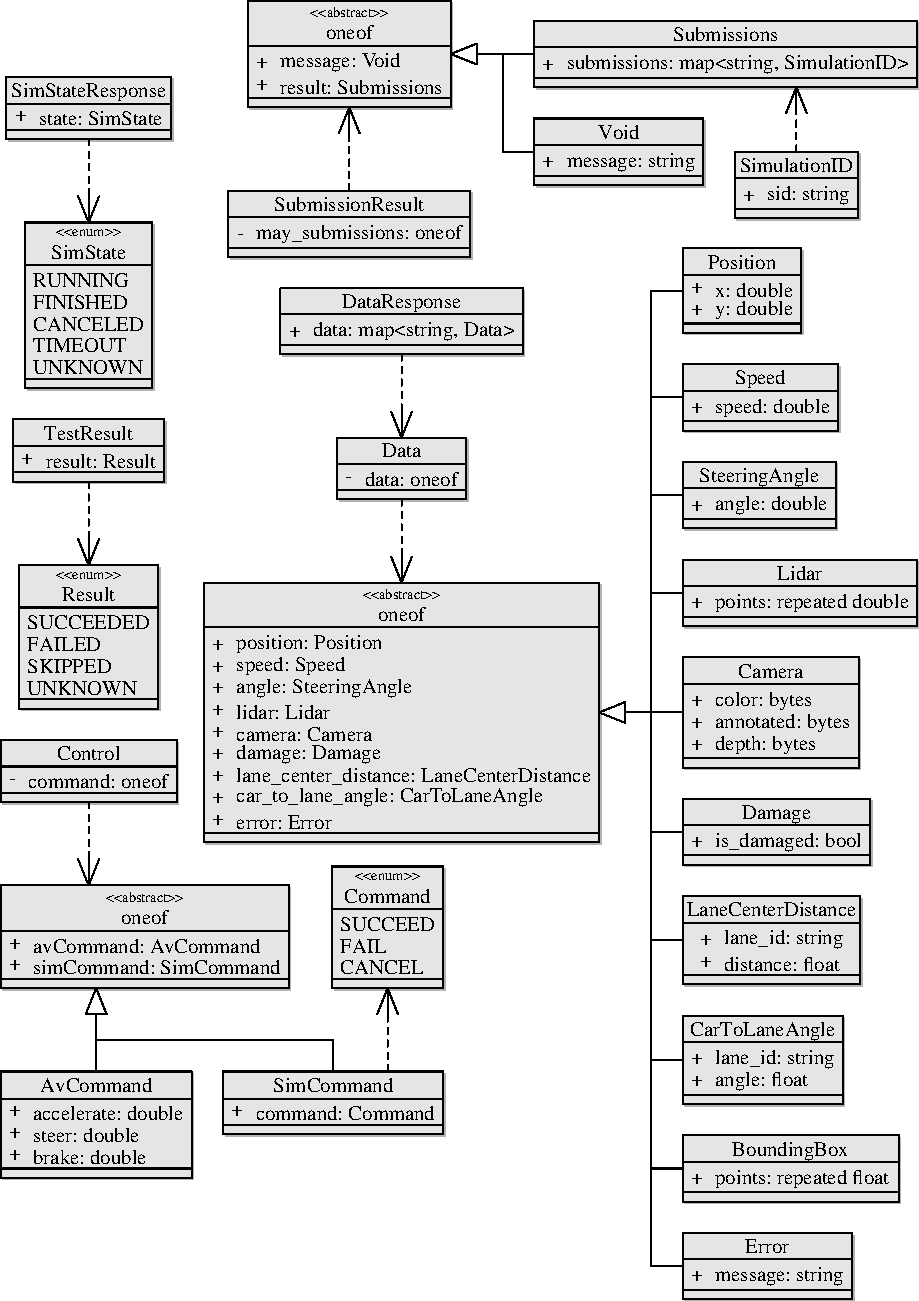
\includegraphics[width=\textwidth, height=.95\textheight, keepaspectratio]{diagrams/messagesTypeGraph-2.pdf}
    \medskip
    \caption{%
        Complex \glspl{pmessage} --- Shows the composition structure of the complex \glspl{pmessage} that \drivebuild{} can handle.
        Private attributes denote the existence and the name of exclusive groups of attributes (\code{oneof}).
    }\label{fig:complexMessages}
\end{figure}
\Glspl{pmessage} are considered as complex if they have at least one attribute whose type is either another \gls{pmessage}, an enum or an exclusive group of attributes (\code{oneof}).
An \code{oneof} group is not a \gls{pmessage} on its own but logically the superclass of multiple other \glspl{pmessage}.
\Glspl{pmessage} can only be properly instantiated from top level \glspl{pmessage}.
Each message on the socket level is a sequence of two sub-messages as shown in \cref{fig:socketMessage}.
\begin{figure}
    \centering
    \begin{sequencediagram}
    \newthread{a}{:A}
    \tikzstyle{inststyle}+=[below right=-0.82cm and 4cm of a]  % FIXME Workaround for newthread distance
    \newthread{b}{:B}
    \begin{callself}{b}{Wait for complete sub-messages}{}
        \mess{a}{content length}{b}
        \mess{a}{content}{b}
    \end{callself}
\end{sequencediagram}

    \medskip
    \caption{%
        Socket message --- Shows the sequence of sub-messages that form a complete message.
        This diagram assumes that A sends a message and B waits for receiving it.
    }\label{fig:socketMessage}
\end{figure}
The content length sub-message has a fixed length and sends the number of bytes that the actual content has.
The actual content sub-message is a \gls{pmessage} which contains the serialized content.
This way the receiver knows the length of both sub-messages and thus can determine whether it already got the complete message or it has to wait for more bytes to receive.
An action request is a sequence of socket messages which implements a function call over a socket.
\Cref{fig:actionRequest} visualizes the sequence of socket messages.
\begin{figure}
    \centering
    \begin{sequencediagram}
    \newthread{a}{:A}
    \tikzstyle{inststyle}+=[below right=-0.82cm and 5cm of a]  % FIXME Workaround for newthread distance
    \newthread{b}{:B}
    \begin{callself}{b}{Wait for complete message}{}
        \mess{a}{action}{b}
        \mess{a}{number of params N}{b}
        \mess[1]{a}{parameters 1 to N}{b}
    \end{callself}
    \begin{callself}{a}{Wait for complete message}{}
        \mess{b}{result}{a}
    \end{callself}
\end{sequencediagram}

    \medskip
    \caption{%
        Action request --- Shows the socket messages that a component A exchanges with component B if A requests an action that B provides.
        Each of these messages consists of sub-messages as described in \cref{fig:socketMessage}.
    }\label{fig:actionRequest}
\end{figure}
The first socket message sends an action that specifies which function has to be called.
The second socket message defines the number of arguments \(N\) which the sender passes to the function.
The next \(N\) socket messages are \glspl{pmessage} which contain the actual arguments.

\subsection{\texorpdfstring{\Glstext{mainapp}}{MainApp}}
The \gls{mainapp} is the central component of \drivebuild{} and offers an interface to all types of clients (see \cref{fig:systemArch}), manages \glspl{simnode} and distributes tests across them.
The interface for clients is a micro service~\cite{microServices} based webserver and \cref{tab:microServices} lists all its services.
\begin{table}
    \centering
    \caption{%
        \Glstext{mainapp} micro services --- Lists the micro services which the \gls{mainapp} provides, a short description, the required parameters and the return type in case a request is successful.
        All parameters have to be appended to an \glstext{url} as GET parameters except for underlined parameters which have to be sent as the content of a POST request.
        Italic entries add notes about parameters.
    }\label{tab:microServices}
    \medskip
    %!TEX root = ../thesis.tex
\def\tabularxcolumn#1{m{#1}}
\begin{tabularx}{.9\textwidth}{X l l}
    \toprule
    \bfseries \Glstext{url} & \bfseries Parameters (name: type) & \bfseries Return Type \\
    \midrule
    /runTests & \makecell[l]{user: User\\\underline{zip byte data}} & SubmissionResult \\
    \midrule
    /ai/waitForSimulatorRequest & \makecell[l]{sid: SimulationID\\vid: VehicleID} & SimStateResponse \\
    \midrule
    /ai/requestData & \makecell[l]{sid: SimulationID\\vid: VehicleID\\request: DataRequest} & DataResponse\\
    \midrule
    /ai/control & \makecell[l]{sid: SimulationID\\vid: VehicleID\\\underline{Control}} & Void \\
    \midrule
    /stats/getRunningSids & user: User & SubmissionResult \\
    \midrule
    /stats/<action> & \makecell[l]{\textit{At least:}\\sid: SimulationID\\\textit{Maybe further parameters}} & \textit{Depends on action} \\
    \midrule
    /sim/stop & \makecell[l]{sim: SimulationID\\result: TestResult} & Void\\
    \bottomrule
\end{tabularx}

\end{table}
The use of micro services hides and strictly separates functionality plus it allows finer granularity than other architectures like \gls{soa}.
From a testers perspective there is only the service \code{/runTests} which submits new tests to \drivebuild{} and starts them.
The tests have to be compressed into a zip file.
This call blocks until \drivebuild{} created all the resulting scenarios and started simulator instances which run all of them.
The response of this request maps the names of the submitted tests to the generated \code{SimulationID}\unskip{}s.
A tester requires this information to map \code{VehicleID}\unskip{}s that tests declare to \code{SimulationID}\unskip{}s and start the corresponding \glspl{ai}.
The interface for \glspl{ai} offers all micro services which they require to implement their interaction with the simulations (see \cref{fig:aiSimProtocol}).
A call to \code{/ai/waitForSimulatorRequest} registers an \gls{ai} for controlling a certain \gls{av} in a certain simulation.
This request blocks until either the simulation requests the registered \gls{ai} or it finishes.
The response contains the current state of the simulation to which this \gls{ai} registered to which allows to determine whether the \gls{ai} has to continue or to stop.
If an \gls{ai} continues it needs data for its computations.
A request to \code{/ai/requestData} retrieves the data of sensors which are attached to a participant or current values of properties of a participant like the current position or damage.
This data also allows to implement additional client side checks.
\code{/ai/control} enables an \gls{ai} to control \glspl{av} and simulations.
The returned message contains a status message which may be used for logging.
The interface of the \gls{mainapp} offers also micro services for researchers to collect and analyze test data.
So the micro service \code{/stats/<action>} provides an interface to query the database about currently running as well as previous tests.
Calls to this service require a \code{SimulationID} as a parameter and possibly further parameters which are specific to the concrete action.
The action \code{result} returns the test result of a simulation if any.
A request with the action \code{status} returns the state of the simulation like \ssrunning{}, \ssfinished{} or \sstimeout{}.
The trace of all data that a simulation collected can be retrieved by calling \code{/stats/trace}.
If a call specifies the optional parameter \code{VehicleID} the response contains only the collected data of the specified participant.
The request \code{/sim/stop} forces simulations to end and can be called from a tester as well as from an \gls{ai}.
This call requires a \code{SimulationID} and a parameter which defines the test result to set.
The result of this call contains a message which can be used for logging.
For debugging purposes of \drivebuild{} the \gls{mainapp} further offers the request \code{/stats/getRunningSids} which returns all IDs of simulations which a given user currently runs on any \gls{simnode}.\\
The interface for \glspl{simnode} is on the socket level and \cref{subsec:simnode} describes it in detail.
Besides the actual interface the \gls{mainapp} opens a port which \glspl{simnode} use to register themselves at the \gls{mainapp}.
When a new \gls{simnode} connects the \gls{mainapp} generates an unique ID, associates the incoming socket connection with it and returns the ID to the newly registered \gls{simnode}.

\subsection{\texorpdfstring{\Glstext{simnode}}{SimNode}}\label{subsec:simnode}
\Glspl{simnode} generate \beamng{} scenarios and run the actual test executions which include the simulations, the runtime verification, the interaction with \glspl{ai} and the collection of data.
% Interface to MainApp
The communication between \glspl{simnode} and the \gls{mainapp} is based on low level socket communication.
Therefore the \glspl{simcontroller} of the \glspl{simnode} offer the interface that \cref{tab:simNodeToMainAppInterface} lists which enables the \gls{mainapp} to manage simulations and to organize the interaction between on the one hand simulations and on the other hand testers and \glspl{ai}.
\begin{table}
    \centering
    \caption{%
        Interface to \gls{mainapp} --- Describes the interface to which the \gls{mainapp} sends action requests to access the functions of the \gls{simcontroller} of a \gls{simnode}.
        \Cref{fig:actionRequest} describes the structure of action requests.
    }\label{tab:simNodeToMainAppInterface}
    \medskip
    %!TEX root = ../thesis.tex
\def\tabularxcolumn#1{m{#1}}
\begin{tabularx}{.75\linewidth}{X l l}
    \toprule
    \bfseries Action & \bfseries Parameter Types & \bfseries Return Type \\
    \midrule
    runTests & \makecell[l]{User\\zip byte data} & SubmissionResult \\
    \midrule
    waitForSimulatorRequest & \makecell[l]{SimulationID\\VehicleID} & SimStateResponse \\
    \midrule
    control & \makecell[l]{SimulationID\\VehicleID\\Control} & Void \\
    \midrule
    requestData & \makecell[l]{SimulationID\\VehicleID\\DataRequest} & DataResponse \\
    \midrule
    stop & \makecell[l]{SimulationID\\TestResult} & Void \\
    \midrule
    runningTests & User & SubmissionResult \\
    \midrule
    requestSocket & --- & Void \\
    \bottomrule
\end{tabularx}

\end{table}
To use the interface the \gls{mainapp} has to make action requests.
The interface has many similarities to the micro services which the \gls{mainapp} offers to clients since many of the micro services are only redirections of requests to appropriate \glspl{simcontroller}.
This is the case for the actions \code{runTests}, \code{waitForSimulatorRequest}, \code{control}, \code{requestData} and \code{stop}.
The action \code{runningTests} searches for all \code{SimulationID}\unskip{}s of simulations which a given user currently runs on any \gls{simnode} and returns a map which associates test names with its \code{SimulationID}.
A call to the action \code{requestSocket} makes the requested \gls{simcontroller} open an additional socket which registers itself to the \gls{mainapp}.
The \gls{mainapp} uses this socket to open a socket for each \gls{ai} in each currently running simulation.\\
Since a \gls{simcontroller} runs multiple \beamng{} instances the corresponding runtime verification processes have to run simultaneously as well.
Further a \gls{simcontroller} has to share references to all \beamng{} instances with the corresponding runtime verification processes.
The exchange of data between processes in Python is based on serialization and results in deep copies of Python objects.
Since \beamng{} and \beamngpy{} use internally lots of sockets and Python is intentionally not able to serialize sockets neither \beamng{} nor \beamngpy{} instances can be easily shared.
So each \gls{simcontroller} offers a second interface (see \cref{tab:simNodeToSimulationInterface}) which runtime verification processes use to interact with \beamng{} instances and to evaluate criteria which require the current state of a simulation.
\begin{table}
    \centering
    \caption{%
        Interface to runtime verification processes --- Describes the interface that a runtime verification uses to interact with simulations using action requests.
        \Cref{fig:actionRequest} describes the structure of action requests.
    }\label{tab:simNodeToSimulationInterface}
    \medskip
    %!TEX root = ../thesis.tex
\def\tabularxcolumn#1{m{#1}}
\begin{tabularx}{.65\linewidth}{X l l}
    \toprule
    \bfseries Action & \bfseries Parameter Types & \bfseries Return Type \\
    \midrule
    vids & SimulationID & VehicleIDs \\
    \midrule
    isRunning & SimulationID & Bool \\
    \midrule
    pollSensors & SimulationID & Void \\
    \midrule
    verify & SimulationID & VerificationResult \\
    \midrule
    requestAiFor & \makecell[l]{SimulationID\\VehicleID} & Void \\
    \midrule
    steps & \makecell[l]{SimulationID\\Num} & Void \\
    \midrule
    stop & \makecell[l]{SimulationID\\TestResult} & Void \\
    \bottomrule
\end{tabularx}

\end{table}
A request with the action \code{vids} returns the IDs of all participants in a given simulation.
The action request \code{isRunning} determines whether a specific simulation runs.
The action \code{pollSensors} updates the cached data which \glspl{ai} can request about a simulation, the properties of any participant and their sensors.
The action request \code{verify} evaluates the test criteria based on the currently cached data and returns the evaluation result of the precondition, the success and the failure criteria.
A call to \code{requestAiFor} notifies all registered \glspl{ai} about newly available data.
This call blocks until for all \glspl{av} an \gls{ai} registered with the action \code{waitForSimulatorRequest}.
If so all the calls to \code{waitForSimulatorRequest} continue.
The action request \code{steps} makes a simulation continue for the given amount of ticks.
How much progress a simulation makes depends on the values \code{steps per second} which defines into how many ticks a second in the simulation time is divided and the \code{\gls{ai} frequency} which specifies after how many ticks of simulation another cycle in the runtime verification starts.\\
\Cref{fig:runtimeVerificationScheme} depicts the sequence of calls that implements the cycle.
\begin{figure}
    \centering
    %!TEX root = ../thesis.tex
\begin{sequencediagram}
    \newthread{simcontroller}{:Runtime Verification}
    \tikzstyle{inststyle}+=[below right=-0.82cm and 5cm of simcontroller]  % FIXME Workaround for newthread distance
    \newthread{simnode}{:\Glstext{simcontroller}}
    \begin{call}{simcontroller}{vids}{simnode}{VehicleIDs}
    \end{call}
    \begin{sdblock}{Loop cycle}{While simulation running}
        \begin{call}{simcontroller}{verify}{simnode}{VerificationResult}
        \end{call}
        \begin{call}{simcontroller}{pollSensors}{simnode}{Void}
        \end{call}
        \begin{sdblock}{For each \glstext{av}}{}
            \begin{call}{simcontroller}{requestAiFor}{simnode}{Void}
                \postlevel%
            \end{call}
        \end{sdblock}
        \prelevel\prelevel\prelevel%
        \begin{callself}{simcontroller}{Wait for control commands}{Apply control commands}
            \postlevel\postlevel%
        \end{callself}
        \begin{call}{simcontroller}{steps}{simnode}{Void}
        \end{call}
    \end{sdblock}
\end{sequencediagram}

    \medskip
    \caption{%
        Runtime verification calls --- Structures the calls of the runtime verification to the \gls{simcontroller}.
        It uses the interface which \cref{tab:simNodeToSimulationInterface} lists.
    }\label{fig:runtimeVerificationScheme}
\end{figure}
The only call before the first cycle starts requests the IDs of all participants in the simulation.
The first call within the cycle evaluates the test criteria and applies the decision tree in \cref{fig:verificationDecision} to determine the current test result.
If the test result is something else than \trunknown{} it stops the simulation and notifies all registered \glspl{ai} about it.
Otherwise the cycle continues.
In this case the runtime verification retrieves the current states and the sensor data of all \glspl{av} and updates the cached data which is available for \glspl{ai}.
The next calls notify all \glspl{ai} which control \glspl{av} that are either in the movement mode \mmautonomous{} or \mmtraining{} with \code{requestAiFor} about new data and waits for the \glspl{ai} to send control commands.
Therefore the runtime verification starts a separate process that waits until the \gls{simcontroller} got all control commands of all \glspl{ai} from the \gls{mainapp}.
The runtime verification first applies commands that control the simulation.
If these stop the simulation the runtime verification notifies all registered \glspl{ai} about it and exits.
Otherwise it applies the control commands which control \glspl{av} and calls \code{step} which makes the simulation continue for a few ticks.
Then the loop starts over again.\\
To implement the interaction between an \gls{ai} and a simulation on the client side the implementation of the \gls{ai} has to follow the scheme that \cref{fig:clientScheme} shows.
\begin{figure}
    \centering
    \plainFrame{%
    \centering
    \resizebox{!}{\pageheight}{%
        \begin{sequencediagram}
            \newthread{client}{:Client}
            \tikzstyle{inststyle}+=[below right=-0.82cm and 5cm of client]
            \newthread{drivebuild}{:MainApp}
            \begin{call}{client}{/runTests}{drivebuild}{SubmissionResult}
            \end{call}
            \begin{sdblock}{Handle AI}{For each AI in parallel}
                \begin{call}{client}{/ai/waitForSimulatorRequest}{drivebuild}{SimStateResponse}
                    \begin{callself}{drivebuild}{Wait for requestAiFor}{}
                    \end{callself}
                \end{call}
                \begin{call}{client}{/ai/requestData}{drivebuild}{DataResponse}
                \end{call}
                \begin{callself}{client}{Calculate control commands}{}
                \end{callself}
                \begin{call}{client}{/ai/control}{drivebuild}{Void}
                    \begin{callself}{drivebuild}{Apply control commands}{}
                    \end{callself}
                \end{call}
            \end{sdblock}
        \end{sequencediagram}
    }
    \subsectionBox{colorVerify!40}
}


    \medskip
    \caption{%
        Client scheme --- Depicts the basic scheme of the sequence of calls that a client has to make to implement interaction with \drivebuild{}.
        Therefore it has to use the interface which \cref{tab:microServices} lists.
    }\label{fig:clientScheme}
\end{figure}
The interaction uses the same \glspl{pmessage} as the low level socket communication uses (see \cref{subsec:communication}).
\Cref{fig:exampleMessageUsage} shows examples of how to create and read the most important \glspl{pmessage} which the client requires.
\begin{figure}[h]
    \captionsetup{type=listing}
    \newcounter{sublisting}
    \renewcommand{\thesublisting}{\alph{sublisting}}
    \begin{subfigure}{\textwidth}
    \centering
    \inputminted{python}{code/exampleMessageCreation.py}
    \caption{%
        Creation of simple messages
    }
\end{subfigure}
\begin{subfigure}{\textwidth}
    \centering
    \inputminted{python}{code/exampleMessageAccess.py}
    \caption{%
        Access to attributes of complex messages
    }
\end{subfigure}

    \medskip
    \caption{%
        Example \glspl{pmessage} --- Demonstrates the creation and usage of the fundamental \glspl{pmessage} that a client implementation requires.
    }\label{fig:exampleMessageUsage}
\end{figure}
The first call submits formalized test cases to \drivebuild{} and returns a map from the declared test names to the assigned \code{SimulationID}\unskip{}s.
The client starts for each participant in each simulation a separate process which interacts with the participant.
This process repeats a certain sequence of calls as long as the simulation which simulates the participant runs.
The first call in the sequence registers the process with \code{waitForSimulatorRequest} for the interaction with a specific participant in a certain simulation and blocks until one of the two following events occur.
The one event occurs if the participant enters one of the movement modes \mmautonomous{} or \mmtraining{} and the runtime verification calls \code{requestAiFor}.
The other event occurs if the simulation stops.
The call to \code{waitForSimulatorRequest} is the only required call.
Any other call may be omitted.
If the request returns and the simulation is not in state \ssrunning{} the interaction stops, the process may clean up memory and exit.
Otherwise the interaction continues and may request properties about participants or their sensor data.
At this point a client can collect training data for \glspl{ai}.
If a participant is in movement mode \mmautonomous{} the process can either calculate commands which handle the \gls{av} or send commands which control the simulation.
If the participant is in movement mode \mmtraining{} it can only control the simulation and the \gls{mainapp} ignores any command which controls an \gls{av}.
Then the sequence of interaction calls starts over again.\\
% Process of simulation generation and start
Internally a \gls{simnode} implements all phases of the test life cycle (see \cref{fig:testCycle}) and therefore the appropriate components of \drivebuild{} as \cref{fig:systemArch} shows.
The \transformer{} implements the input validation step.
Therefore it validates tests against the \gls{xsd} which \drivebuild{} provides.
The \generator{} and the \gls{kptransformer} implement the extraction step as well as the transformation step.
In the extraction step they use XPath to extract all information that the semantic model requires.
The actual semantic model results from the transformation step.
The \generator{} uses structs to represent the environment of a simulation.
The \gls{kptransformer} parses precondition, success and failure criteria from top to bottom and recursively creates \lambda{} expressions that abstractly represent the test criteria as Kleene and Priest logics expressions.
These \lambda{} expressions take a \beamng{} scenario as their input and can evaluate the criteria based on the current state of the scenario.
Further the \gls{kptransformer} attaches default data requests which collect data to partially reproduce a simulation without having to actually execute it again or which future work might require.
It also may attach additional sensors to participants if the evaluation of criteria requires further data.
On the one hand the \gls{simcontroller} creates and manages the simulations and the runtime verification processes and on the other organizes the interaction with the \gls{mainapp}.\\
Before starting a simulation the \gls{simcontroller} has to generate a \beamng{} scenario.
The level for the scenario is an infinitely big flat plain which is covered with grass.
A \beamng{} scenario consists of a \json{}, a prefab and a \lua{} file.
The \json{} file contains meta data about the scenario including its name, the author, a description and a reference to the prefab file.
The prefab file describes the static information about initial states of vehicles, roads, waypoints and \lua{} triggers.
The \gls{simcontroller} uses \beamngpy{} to create an initial \beamng{} scenario but further modifies it since \beamngpy{} does not provide all required features.\\
% initial states
The definition of positions of participants in the formalization corresponds to \beamng{} but the definition of orientations of participants defers.
The formalization defines orientation as \cref{fig:envCooSystem} shows.
In contrast \beamng{} defines orientation in clockwise manner and an orientation of \ang{0} makes the car head in negative y direction.
So the generator has to translate the orientation accordingly before placing participants in a \beamng{} scenario.
% roads
When adding a road it is smoothened by interpolating the points which the semantic model stores for its course with a cubic B-spline.
The interpolation sets the smoothness to \num{0} and adds additional points to ensure that the resulting course fits all points perfectly and the its shape is like expected.
The interpolation is done with \scipy{}~\cite{scipy}
The road markings in the scenario are implemented as narrow lanes which are parallel to the B-spline and just have a different texture than the actual road.
\scipy{} provides methods to calculate these parallel lines, \ie{} offset lines.
A road has a declared number of left and right lanes.
The generator creates two offset lines for the left and right side road marking (continuous white line), one offset line which separates left from right lanes (continuous double yellow line) and offset lines that separate left and right lanes from each other (dashed white line).
% waypoints
The dynamic behavior of participants is described by sequences of waypoints in the semantic model.
The generator adds for each of these waypoints corresponding \beamng{} waypoints which have the position and size as defined in the semantic model.
% LUA triggers
Further it adds \lua{} triggers for each \beamng{} waypoint.
\lua{} triggers define areas where custom \lua{} functions are executed as soon as the bounding box of a participant intersects with it or does not intersect with it anymore.
When a participant reaches a \lua{} trigger the simulation calls a custom \lua{} function which makes the participant move to the next \beamng{} waypoint.
Since these functions make a participant approach to a \beamng{} waypoint such a way that it almost touches the waypoint without intersecting it \lua{} triggers have to be slightly bigger than the underlying \beamng{} waypoint to make sure the participant intersects the \lua{} trigger.
When a participant reaches a \lua{} trigger the custom \lua{} function also applies the additional properties of the waypoints in the semantic model which includes target speeds, speed limits and changes of the movement mode.
Due to the internal implementation of \beamng{} a speed limit overrides a target speed.
If the generation of the \beamng{} scenario finished the \gls{simcontroller} starts a new \beamng{} instance, loads the scenario and starts the simulation.

\subsection{\texorpdfstring{\Glstext{dbms}}{DBMS}}
The database uses \postgresql{} since \postgresql{} is well known, well supported in many languages and provides the data type \code{SERIAL} which allows to easily and safely generate unique \code{SimulationID}\unskip{}s for tests.
\Cref{fig:databaseScheme} depicts the complete scheme which \drivebuild{} uses to store data about finished and currently running tests as well as data about properties and sensor data of all participants in any runtime verification cycle.
\begin{figure}
    \centering
    \begin{tikzpicture}
    \node[attribute] (sid) {\key{SimulationID}};
    \node[attribute, below=0.5 of sid] (environment) {Environment};
    \node[attribute, below=0.5 of environment] (criteria) {Criteria};
    \node[attribute, below=0.5 of criteria] (result) {TestResult};
    \node[attribute, below=0.5 of result] (status) {SimState};
    \node[attribute, below=0.5 of status] (started) {StartTime};
    \node[attribute, below=0.5 of started] (finished) {EndTime};
    \node[entity, right=of result] (test) {Tests};

    \node[ident relationship, right=of test] (of) {in};

    \node[weak entity, right=of of] (trace) {VerficationCycles};
    \node[attribute, above=of trace.north west, anchor=south] (tick) {\weakkey{Tick}};
    \node[attribute, above=of trace.north east, anchor=south] (cycleFinished) {EndTime};
    \node[attribute, below=of of] (vid) {\weakkey{VehicleID}};
    \node[attribute, below=of vid.south east, anchor=north] (data) {DataResponse};
    \node[attribute, above=of data.east, anchor=south west] (cycleStarted) {StartTime};

    \node[relationship, above right=1.5 and 0 of test] (submit) {submit};

    \node[entity, above=of submit] (user) {Users};
    \node[attribute, right=of user] (username) {\key{Username}};
    \node[attribute, above=0.5 of username] (password) {Password};

    \path
        (test) edge[bend right] (sid)
        (test) edge (environment)
        (test) edge (criteria)
        (test) edge (result)
        (test) edge (status)
        (test) edge (started)
        (test) edge[bend left] (finished)
        (trace) edge (data)
        (trace) edge (vid)
        (trace) edge (tick)
        (trace) edge (cycleStarted)
        (trace) edge (cycleFinished)
        (trace) edge[total] node[above] {n} (of)
        (of) edge node[above] {1} (test)
        (user) edge (username)
        (user) edge (password)
        (user) edge node[right] {0...1} (submit)
        (submit) edge node[above] {n} (test);
\end{tikzpicture}

    \medskip
    \caption{%
        Database scheme --- Depicts all the data that \drivebuild{} stores about executed and running tests and how the data relates.
    }\label{fig:databaseScheme}
\end{figure}
The table \enquote{Test} stores for each test execution the \code{SimulationID}, the current test result, the current state of the simulation and timestamps for when the execution started and finished.
Additionally it contains serialized byte strings of the \gls{dbe} and \gls{dbc} which specify the test.
% The table also stores the result of the test.
% As long as the simulation runs this value is \trunknown{}.
% If the simulation ends without timeout it set to either one of \trsucceeded{}, \trfailed{} or \trskipped{}.
% Furthermore the table contains the current state of simulations which is one of \ssrunning{}, \ssfinished{}, \sscanceled{} or \sstimeout{} and time stamps for when the simulation started and when it ended.
Each entry in \enquote{Test} references the user in \enquote{User} who submitted the test to \drivebuild{}.
Each user has an username and a password.
The table \enquote{VerficationCycles} stores all data which the runtime verification collects in each cycle.
This includes especially all properties and sensor data of any participants.
Since the properties as well as the sensor data is highly diverse and may change when more sensors are added or when the provided detail of sensor data increases it is very hard to specify a fixed static \gls{dbms} scheme.
So the collected data is stored in a single field where a serialized \code{DataResponse} object contains all the data.
Each entry additionally stores two timestamps that save the time from the start of a cycle until the call to \beamng{} for continuing the simulation.

    %!TEX root = ../thesis.tex
\section{Evaluation}\label{sec:evaluation}
The evaluation aims to show that the test formalization of \drivebuild{} is general enough to be used with different approaches for implementing test generators and \glspl{ai}.
It also aims to show whether test executions on a single \gls{simnode} on a real machine scale linearly and whether the performance degradation when using \glspl{vm} to host \glspl{simnode} is unbearable.
The evaluation addresses the following main research questions:
% https://library.royalroads.ca/writing-centre/writing/structure/thesis-statements lists a few characteristics RQs should have.
\begin{description}
    \item[RQ1] How comprehensive is the test formalization concerning the support of various kinds of test generators and \glspl{ai}?
        Different approaches for test generators and \glspl{ai} have different requirements when testing them.
        The creation of benchmarks and ratings for comparing test generators and \glspl{ai} to each other introduces even further requirements.
        Thus in order to interact with test generators and \glspl{ai}, to analyze and to offer feedback data the formalization has to fulfill these requirements.
        The evaluation focuses on approaches that \cref{sec:stateOfTheArt} presents to investigate the research question.
    \item[RQ2] How does \drivebuild{} scale over real machines and \glspl{vm}?
        \drivebuild{} is a distributed system and aims to run as many simulations as possible in parallel.
        This research question investigates how many tests a single \gls{simnode} can run without having an influence on the test results, the benefit of utilizing parallelism and whether hosting \glspl{simnode} in \glspl{vm} is a feasible solution to distribute simulations over a cluster.
    \item[RQ3] How supportive is \drivebuild{} for developers in setting up simulations, running tests and collecting data?
        A goal of \drivebuild{} is to lift out testers of tedious and error prone tasks like setting up and managing simulations as well as implementing an interaction between simulations and \glspl{ai}.
        This research question qualitatively evaluates the benefits of using \drivebuild{} compared to manually setting up and executing tests.
        Therefore it compares the effort to understand and use \drivebuild{} to the benefits \drivebuild{} offers.
\end{description}
The evaluation has four subsections.
\Cref{subsec:experimentalSettings} elaborates in which context the evaluation took place and lists all technical specifications which are relevant.
\Cref{subsec:evaluationOfGenerality} describes the test for checking the comprehensiveness of the test formalization and introduces a number of metrics which \drivebuild{} can yield about test generators and \glspl{ai}.
\Cref{subsec:evaluationOfScalability} quantitatively evaluates the scalability of \drivebuild{} concerning the number of simultaneously executed simulations and the number of \glspl{simnode} connected to the \gls{mainapp}.
It also compares the scalability between a \gls{simnode} running on a real machine and \glspl{simnode} hosted on \glspl{vm}.
\Cref{subsec:experienceReport} examines qualitatively the benefits of \drivebuild{}, how supportive it is for testers and the presumably most difficult tasks when using it.
\subsection{Experimental Settings}\label{subsec:experimentalSettings}
\subsubsection{Seminar}
The evaluation took place in the context of the advanced seminar \enquote{Search-based Software Engineering for Testing Autonomous Cars (5846HS)} in summer term 2019 at the University of Passau and had 10 participants which were all either master students or bachelor students in a higher semester.
The students were assigned papers that propose and discuss test generators and approaches for training \glspl{ai}.
As part of the seminar, the students had the task to implement small prototypes of test generators or \glspl{ai} which I will refer to as \enquote{submissions}.
So they have to face problems which are similar to problems real tester have.
The problems include the setup of \beamng{}, the management of simulations and the collection of data which are problems that \drivebuild{} claims to solve.
Hence I targeted the students as users like testers would use \drivebuild{}.
\subsubsection{Submissions}\label{subsubsec:submissions}
\Cref{sec:background} explains all approaches the students used for their submissions.
Three students implemented test generators.
Test generator G1 focuses on generating tests that verify whether \glspl{av} can avoid crashes.
Therefore it uses a predefined list of \num{528} IDs of crash reports referencing the \gls{nhtsa} crash report database which provides these reports as semi-structured \gls{xml}.
G1 utilizes \gls{ac3r}~\cite{ac3r} which generates \beamng{} scenarios.
It parses these \beamng{} scenarios and formalizes them such a way that they can be used with \drivebuild{}.
Test generator G2 aims to generate test scenarios that focus on verifying the lane keeping capabilities of \glspl{av}.
It claims to extend \asfault{}~\cite{asfault} by randomly placing static obstacles all over the area where the road is settled.
Test generator G3 focuses on testing lane keeping capabilities of \glspl{av} as well by applying evolutionary computing to generate a population of interesting roads.
Each call to G3 returns only the first element of the resulting population.
It does not apply any metric to determine a specific element in the population.
Besides the test generators students submitted I created a reference generator G0 which generates random tests using \asfault{}.
The generated tests have one road which is restricted to be placed in an area of \(\SI{100}{\metre}\times\SI{100}{\metre}\).
This road has two lanes and a fixed width of \SI{8}{\metre}.
The initial seed is a random number between \num{0} and \num{10000}.\\
Two of the students implemented \glspl{ai}.
The \gls{ai} A1 is based on a version of deep reinforcement learning which uses \gls{ddpg} and a \gls{vae}.
The student pretrained the \gls{ai} on roads generated by \asfault{}.
\Gls{ai} A2 uses \deepdriving{}.
To pretrain the \gls{ai} the student drove a car manually with \beamng{} on the level which \drivebuild{} uses for its simulations.
Additionally to the \glspl{ai} students implemented I use the \beamng{} \gls{ai} as reference \gls{ai} A0.
This \gls{ai} has perfect knowledge about all roads but does neither recognize any obstacles nor any other participants.
It has an option \enquote{stay on lane} which allows to define a single target waypoint instead of a sequence of consecutive waypoints the \gls{av} has to follow.
The \gls{ai} is able to detect which lanes it has to follow to reach the desired target waypoint.
As a restriction the target waypoint has to be right in the middle of the road otherwise the \beamng{} \gls{ai} does not find a path to it.
\subsubsection{Technical Specifications}
\drivebuild{} is a distributed system and the evaluation utilizes this capability by running the components of \drivebuild{}, test generators, \glspl{ai} and the actual evaluation process across multiple nodes.
\Cref{tab:nodeSpecifications} lists the specifications of all available nodes.
\begin{table}
    \caption{%
        Node specifications --- Lists the specifications for all (virtual) nodes that were used for the evaluation.
    }\label{tab:nodeSpecifications}
    \medskip
    \begin{tabularx}{\textwidth}{X l l l l}
    \toprule
    \bfseries Property     & \bfseries Node~0                   & \bfseries Node~1                     & \bfseries Node~2                     & \bfseries Node~3                       \\
    \midrule
    Hardware/\Glstext{vm}? & \Glstext{vm}                       & Hardware                             & Hardware                             & \Glstext{vm}                           \\
    \Glstext{os}           & Linux Debian                       & \makecell[l]{Windows 10\\Enterprise} & Windows 10 Pro                       & Windows 10 Pro                         \\
    Version                & 10                                 & 1903                                 & 1903                                 & 1903                                   \\
    Build                  & 4.19.0--6                          & 18362.418                            & 18362.418                            & 18362.418                              \\
    Architecture           & 64 bit                             & 64 bit                               & 64 bit                               & 64 bit                                 \\
    \midrule
    \Glstext{cpu}          & \makecell[l]{Intel Xeon\\E5--2630} & \makecell[l]{Intel Core\\i7--7700K}  & \makecell[l]{Intel Core\\i7--7700HQ} & \makecell[l]{Intel Xeon\\E3--12xx v2}  \\
    Clock Rate             & \SI{2.4}{\GHz}                     & \SI{4.2}{\GHz}                       & \SI{2.8}{\GHz}                       & \SI{3}{\GHz}                           \\
    Logical Cores          & \num{8}                            & \num{8}                              & \num{8}                              & \num{2}                                \\
    \midrule
    \Glstext{ram}          & \SI{8}{GB}                         & \SI{16}{GB}                          & \SI{16}{GB}                          & \SI{16}{GB}                            \\
    \midrule
    \Glstext{gpu}          & \textit{Not used}                  & \makecell[l]{GeForce\\GTX 1080}      & \makecell[l]{GeForce\\GTX 1070}      & \makecell[l]{GeForce GTX\\Titan Black} \\
    Driver Version         & \textit{Not used}                  & 436.48                               & 436.48                               & 436.30                                 \\
    \bottomrule
\end{tabularx}

\end{table}
During the evaluation node~0 hosts one instance of the \gls{mainapp} which is accessible from all the other nodes and node~1 runs all the submitted test generators, \glspl{ai} and the \submissiontester{} which encapsulates the execution of the submissions, their interaction with \drivebuild{}, the preprocessing of tests and the collection of data for the evaluation.
Node~2 and one or multiple instances of node~3 may run instances of \glspl{simnode} depending on the current test setup.
Each active instance of these nodes hosts exactly one \gls{simnode}.

\subsection{Evaluation of Generality}\label{subsec:evaluationOfGenerality}
The evaluation of the generality of the test formalization considers two main aspects.
The first aspect is the feature coverage that determines which features of \drivebuild{} were used during the evaluation and which submissions used them.
The second aspect examines on the one hand which metrics the submissions require to operate and whether \drivebuild{} provides them and on the other hand which further metrics \drivebuild{} offers to create detailed analysis about the submissions.
All time measurements in any evaluation use real time over simulation time since measuring real time is at many points easier than measuring simulation time.
Further real time considers in contrast to the simulation time the time test generators require to generate new tests as well as the time \glspl{ai} need to calculate control commands.
\subsubsection{Challenge Test}
In order to investigate these aspects the challenge test runs the submitted \glspl{ai} against the submitted test generators.
In terms of the challenge test a combination of a test generator and an \gls{ai} is called a \enquote{match} and has a fixed time budget.
One execution of the challenge test lets each \gls{ai} compete against each test generator.
Each match repeats the following steps again and again until the given time budget is used.
First, the selected test generator generates a test.
In case the generator succeeded the \submissiontester{} checks multiple validity constraints which ensure that the test can be executed and that it can be compared with generated tests of other test generators.
A test is only valid if it defines at least one participant with the name \enquote{ego}, defines at least one road and the generated citeria (\Glstext{dbc}) references the generated environment (\Glstext{dbe}).
If the \submissiontester{} considers the test valid it further modifies the test to ensure comparability with other tests and compatibility with the \gls{ai} assigned to the match:
It enforces a failure criterion which makes the test fail if any participants is off-road or damaged.
It also forces the \gls{av} \enquote{ego} to be in movement mode \mmautonomous{} during the whole simulation and any other participants to be in movement mode \mmtraining{} to make sure it can collect data about all participants.
To enable the assigned \gls{ai} to operate properly the \submissiontester{} adds data requests to the test for all monitoring data the \gls{ai} requires.
For the analysis of the submissions it adds even more data requests to every participant which store the heading angle as well as the position of the participant.
In case of A0 the \submissiontester{} has to define a target position for the \gls{ai}.
\Cref{subsec:targetPositionDetermination} describes the process of finding an appropriate target position in detail.\\
The \submissiontester{} submits the preprocessed test to \drivebuild{}.
If \drivebuild{} accepts the test the \submissiontester{} creates one instance of the assigned \gls{ai} and connects it to the \gls{av} with ID \enquote{ego}.
I execute the challenge test in different configurations.
An execution defines the time budget for matches either with \SI{10}{\minute} or \SI{30}{\minute} and enforces road markings or no road markings.
Additionally I repeat each execution once which results in a total of \num{8} executions.
At the end this yielded a total number of \num{1208} generated tests.
\subsubsection{Interfaces for Challenge Test}
To allow the \submissiontester{} to work with all submissions homogeneously they have to implement predefined interfaces.
A test generator has to provide a class with a method having the signature given in \cref{fig:testGeneratorStub}.
\begin{figure}
    \captionsetup{type=listing}
    \inputminted{python}{code/testGeneratorStub.py}
    \medskip
    \caption{%
        Test generator stub --- Describes the stub for the implementation of a test generator.
    }\label{fig:testGeneratorStub}
\end{figure}
The method \code{getTest()} does not accept any input and returns a tuple with two paths where the first points to a \gls{dbe} file and the second to a \gls{dbc} file which references the \gls{dbe} file. % chktex 36
The method may return \code{None} if the generator is not able to generate more tests.\\
An implementation of an \gls{ai} has to implement the interface \cref{fig:aiStub} shows.
\begin{figure}
    \captionsetup{type=listing}
    \inputminted{python}{code/aiStub.py}
    \medskip
    \caption{%
        \Glstext{ai} stub --- Shows the scheme of the implementation of \glspl{ai} required for the evaluation and uses the client scheme of \cref{fig:clientScheme}.
    }\label{fig:aiStub}
\end{figure}
The constructor of the \gls{ai} accepts an instance representing the connection to \drivebuild{}.
This connection provides methods for the \gls{ai} to request data and control \glspl{av}.
The method \code{add\_data\_requests(\ldots)} adds data requests (see \cref{fig:exampleAIDataRequests}) which the \gls{ai} requires for operation to the declarations of \glspl{av}. % chktex 36
Therefore it accepts the \gls{xml} tag to which the data requests have to be added to and the ID of the \gls{av} for which the data requests are declared.
This ID should be used to create unique IDs for the declared data requests.
The method \code{start(\ldots)} follows the client scheme (see \cref{fig:clientScheme}) which implements the interaction between an \gls{ai} and \drivebuild{}. % chktex 36
It accepts the ID of the simulation which simulates the \gls{av} to control, the ID of \gls{av} itself and a callback method which gathers runtime data about the simulation for the evaluation afterwards.
\subsubsection{Feature Coverage}
The feature coverage indicates which features of \drivebuild{} were used during the evaluation and thus it suggests which features are somewhat tested and presumably work as they are expected.
\Cref{tab:featureCoverage} summarises the most basic features \drivebuild{} provides and which submissions use them.
\begin{table}
    \centering
    \caption{%
        Feature coverage --- Summarizes which features are used by the submissions and the evaluation.
        If a cell contains check mark a submission or the evaluation uses the feature intentionally.
        If a cell contains a tilde the feature is used only sometimes and the submission is not explicitly designed to use it.
    }\label{tab:featureCoverage}
    \medskip
    %!TEX root = ../thesis.tex
\begin{tabularx}{.6\linewidth}{X c c c c}
    \toprule
    \bfseries Feature                          & \bfseries G0 & \bfseries G1 & \bfseries G2 & \bfseries G3         \\
    \midrule
    \multicolumn{5}{c}{Scenario Elements}                                                                          \\
    Multiple participants                      &              & \checkmark{} &              &                      \\
    Obstacles                                  &              &              & \checkmark{} &                      \\
    Multiple roads                             &              & \checkmark{} &              &                      \\
    Intersections                              & \~{}         & \checkmark{} & \~{}         & \~{}                 \\
    \midrule
    \multicolumn{5}{c}{Test Configuration}                                                                         \\
    Road markings                              & \checkmark{} & \checkmark{} & \checkmark{} & \checkmark{}         \\
    Speed limits                               &              &              &              &                      \\
    Target speeds                              &              &              &              &                      \\
    \midrule
                                               & \bfseries A0 & \bfseries A1 & \bfseries A2 & \bfseries Evaluation \\
    \midrule
    \multicolumn{5}{c}{Data Requests}                                                                              \\
    Camera images                              &              & \checkmark{} & \checkmark{} &                      \\
    Speed                                      &              &              & \checkmark{} &                      \\
    Position                                   &              &              &              & \checkmark{}         \\
    Bounding box                               &              &              &              & \checkmark{}         \\
    \midrule
    \multicolumn{5}{c}{Criteria}                                                                                   \\
    Damage detection                           &              &              &              & \checkmark{}         \\
    Off-road detection                         &              &              &              & \checkmark{}         \\
    Goal area detection                        &              &              &              & \checkmark{}         \\
    \Glstext{vc}                               &              &              &              &                      \\
    \bottomrule
\end{tabularx}

\end{table}
The submissions use only a very restricted subset of the features that \drivebuild{} offers.
There is only one test generator which declares obstacles.
There is also only one test generator which defines more than a single participant on a single road and which intentionally creates intersections.
That the test generators use the road markings feature results from the fact that the configuration of the challenge test enforces them.
The \glspl{ai} rely on camera images and one \gls{ai} additionally relies on the current speed of an \gls{av}.
The evaluation part of the table includes features to evaluate the challenge test as well as the test criteria.
The evaluation uses only features which are related to check and analyse the lane keeping capabilities of \glspl{ai}.
The evaluation does not declare any criteria that use \glsfirstplural{vc}.\\
As a conclusion the small set of used features is sufficient to support all submissions and to create metrics to analyze them.
\drivebuild{} offers many more features which are not listed in \cref{tab:featureCoverage}.
Since neither the submissions nor the evaluation use them their investigation is subject of future.
\subsubsection{Efficiency of Test Generators}
The efficiency of test generators is a metric to identify how many valid tests a generator can produce in a given time interval.
\Cref{fig:exectionTimes} visualizes the distribution of the duration of the executed tests.
\begin{figure}
    \includesvg[width=\textwidth]{diagrams/diagram17a.svg}
    \medskip
    \caption{%
        Execution times --- Visualizes the durations of executed simulations and their standard deviation.
        The execution time includes generation of a test, upload to \drivebuild{}, start of a simulator instance, running the test until it finishes.
        This diagram shows only execution times of tests which did not encounter a timeout.
    }\label{fig:exectionTimes}
\end{figure}
The efficiency \(e\) of the test generators is \num{1} divided by the average time per test execution \(t_{avg}\) (see \cref{eq:efficiency}).
\begin{equation}
    \label{eq:efficiency}
    e = 1 / t_{avg}
\end{equation}
The average execution time \(t_{avg}\) for G0 is \SI{1.75}{\minute}, for G1 \SI{0.70}{\minute}, for G2 \SI{0.28}{\minute} and for G3 \SI{0.60}{\minute}.
G2 is by far the most efficient test generator.
G1 and G3 have a similar efficiency despite the fact that G1 uses \gls{ac3r} which focuses on generating very compact test scenarios and should result in short execution times whereas G3 uses a \gls{ga} to evolve tracks.
G0 is clearly the least efficient test generator although G2 claims to use \asfault{} the same way.
\Cref{fig:numberOfTests} groups the generated tests by test generator and compares the number of generated tests based on the available time budget of the challenge test execution.
\begin{figure}
    \includesvg[width=\textwidth]{diagrams/diagram16a.svg}
    \medskip
    \caption{%
        Number of generated tests --- Shows how many valid and invalid tests each of the test generators generated in total during the challenge test.
        The diagram groups them by the time budget available in a round.
        It also shows their standard deviation.
    }\label{fig:numberOfTests}
\end{figure}
When comparing the number of generated tests in executions with different time budgets the number of generated tests within \SI{30}{\minute} is about three times as high as within \SI{10}{\minute}.
This suggests that the efficiency of the test generators does not decrease the longer they run although some of them should rely on feedback data.
A validation of this statement requires many more executions of the challenge which is not done during this thesis.
\subsubsection{Complexity of Test Cases}
Metrics about the complexity of generated tests allow to estimate how difficult it is for an \gls{av} to succeed a test.
Depending on which properties of an \gls{av} have to be tested different aspects of complexity are considered.
Since most of the submitted test generators test lane keeping capabilities the evaluation investigates the complexity of the generated environments and how far \glspl{av} traveled.
For the metrics I use amongst others the number of scenario elements \ie{} participants, obstacles and roads plus the complexity of the curvature and the length of the generated roads.\\
\Cref{fig:numElements} visualizes the number of scenario elements.
\begin{figure}
    \includesvg[width=\textwidth]{diagrams/diagram9a.svg}
    \includesvg[width=\textwidth]{diagrams/diagram11a.svg}
    \includesvg[width=\textwidth]{diagrams/diagram10a.svg}
    \medskip
    \caption{%
        Number of scenario elements --- Shows which types of scenario elements like participants, roads and obstacles generated tests included and how many.
    }\label{fig:numElements}
\end{figure}
Every test generated by G0, G2 or G3 declares exactly one road and one participant.
In contrast to any other generator G1 often defines two roads and one participant on each road.
This is due to the fact that G1 uses crash reports to generate test cases and the crash reports that the underlying database provides most commonly involve two participants and often intersections.
G2 is the only generator that adds static obstacles to its tests since the student who implemented it had the explicitly the task to generate tests with obstacles.\\
\Cref{fig:roadLengths} shows the distribution of the lengths of the generated roads.
\begin{figure}
    \includesvg[width=\textwidth]{diagrams/diagram8a.svg}
    \medskip
    \caption{%
        Road lengths --- Visualizes the lengths of the generated roads grouped by test generator.
        The longer a road is the potentially more complex its curvature might be.
    }\label{fig:roadLengths}
\end{figure}
The shorter generated roads are the less potential they have to have a complex and diverse curvature.
The longer the generated roads are the longer the execution of a test takes for an \gls{av} to succeed.
G0, G2 and G3 generate roads of very similar length but G3 has a little less variety in their length.
G1 generates much shorter roads which is a result of \gls{ac3r} which aims to generate very compact test scenarios.
This indicates that G1 does not define complex roads.\\
\Cref{fig:numRoadSegments} depicts the distribution of the number of segments that define each generated road.
\begin{figure}
    \includesvg[width=\textwidth]{diagrams/diagram7a.svg}
    \medskip
    \caption{%
        Number of road segments --- Depicts the number of road segments that were used for any road generated during the challenge test.
        It groups them by test generator.
    }\label{fig:numRoadSegments}
\end{figure}
The lower the number of road segments the lower is the potential of the road to have a complex and diverse curvature.
The fewer road segments define a road and the longer the road is the more likely it is that the generated curvature differs from what the test generator intended since it relies more on the interpolation done by \drivebuild{}.
Every road generated by G1 has a low number of segments which fits well with the goal of \gls{ac3r} to create very compact tests.
G3 uses a constant number of road segments.
The initial population is a set of randomly placed positions which define the segments of a road.
Based on this population the \gls{ga} which G3 applies evolves tracks by repositioning the segments.
G2 uses a constant number of road segments as well but the number of segments is much lower.
Since the roads are much longer compared to roads of other generators it is likely that they have many long and only slightly winding sections and may not have a very diverse curvature.
The constant number of road segments further indicates that the implementation of G2 does not use \asfault{} to generate random roads as it was supposed to do.
This becomes especially clear when compared to G0.
The number of road segments generated by G0 has a much higher variety.
Combining this observation with the fact that the length of the generated roads has a variety similar to G2 and G3 indicates that the generated roads may have in some cases more linear and in others more winding sections.\\
\Cref{fig:roadVisualization} supports these observations.
\begin{figure}
    \centering
    %!TEX root = ../thesis.tex
\setlength{\fboxsep}{0pt}
\begin{subfigure}[c]{.49\linewidth}
    \fbox{
        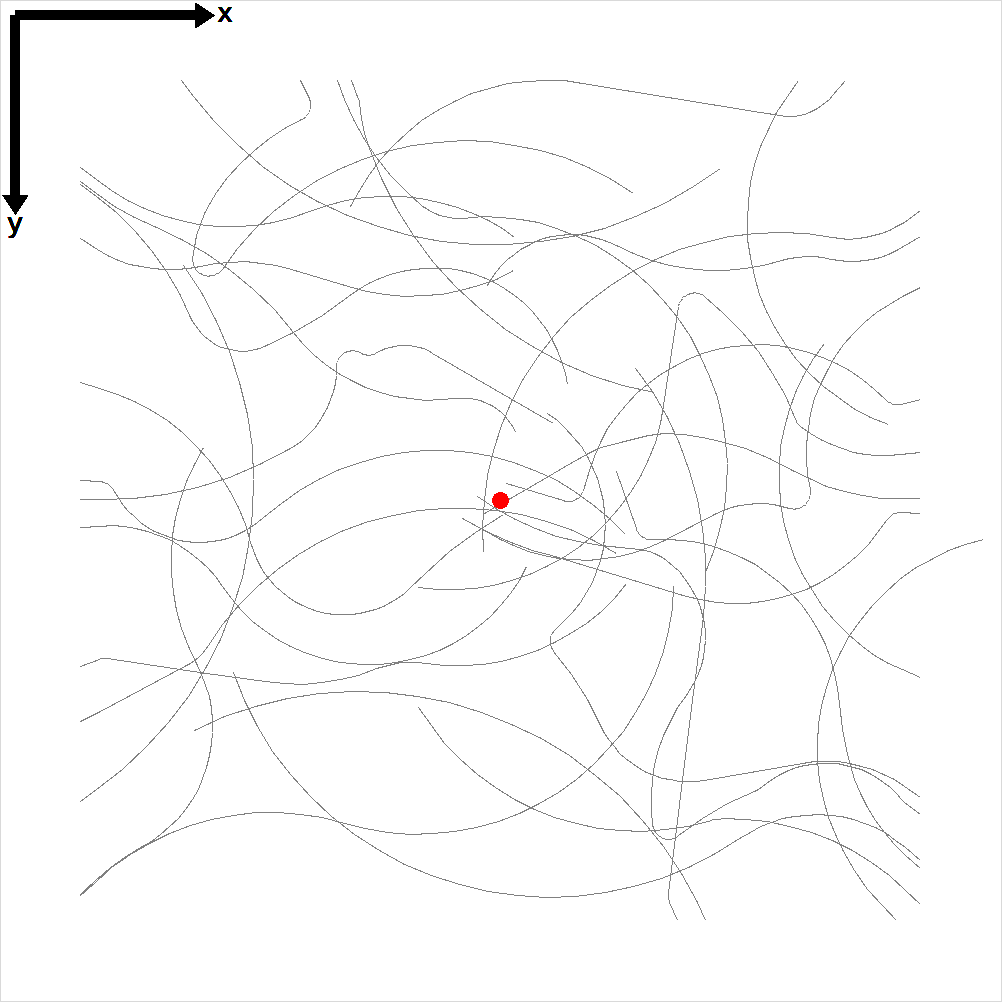
\includegraphics[width=.96\linewidth]{diagrams/roadVisualization_G0.png}
    }
    \subcaption{%
        Roads generated by G0
    }
\end{subfigure}
\begin{subfigure}[c]{.49\linewidth}
    \fbox{
        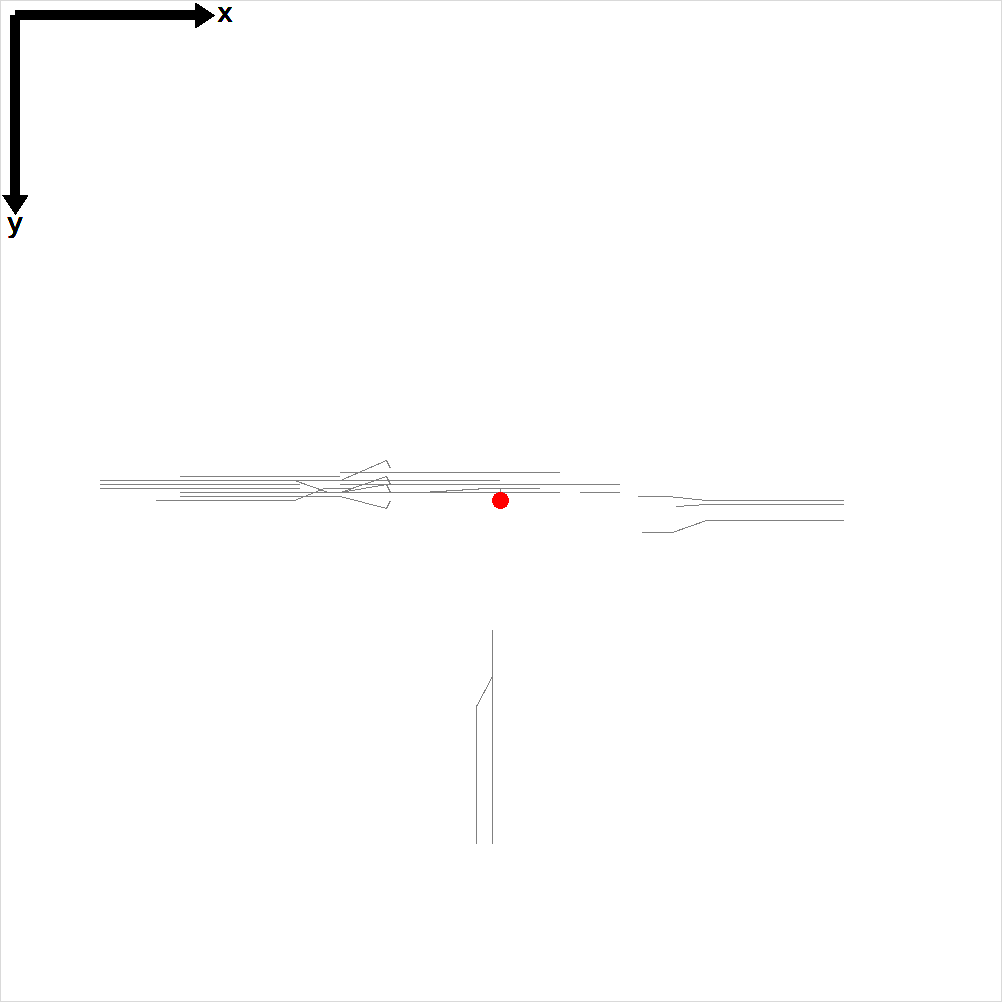
\includegraphics[width=.96\linewidth]{diagrams/roadVisualization_G1.png}
    }
    \subcaption{%
        Roads generated by G1
    }
\end{subfigure}
\begin{subfigure}[c]{.49\linewidth}
    \fbox{
        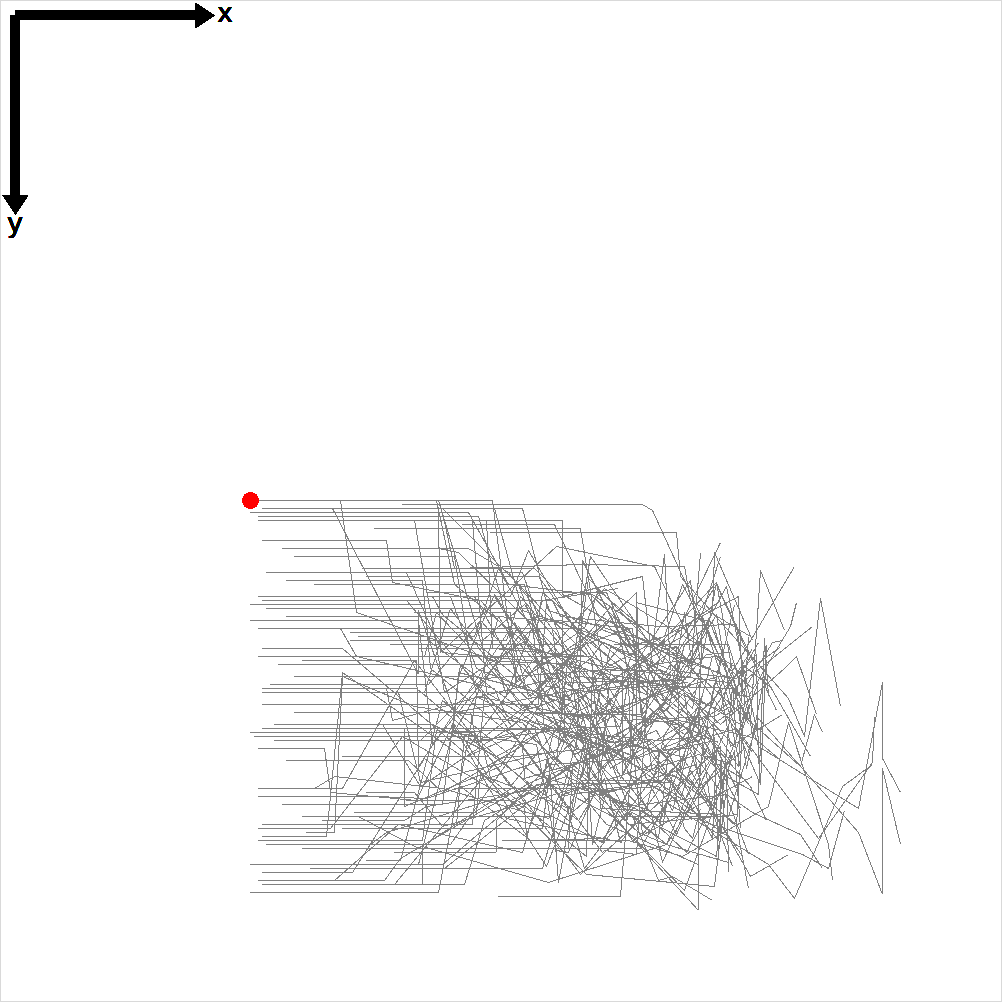
\includegraphics[width=.96\linewidth]{diagrams/roadVisualization_G2.png}
    }
    \subcaption{%
        Roads generated by G2
    }\label{subfig:roadVisualizationG2}
\end{subfigure}
\begin{subfigure}[c]{.49\linewidth}
    \fbox{
        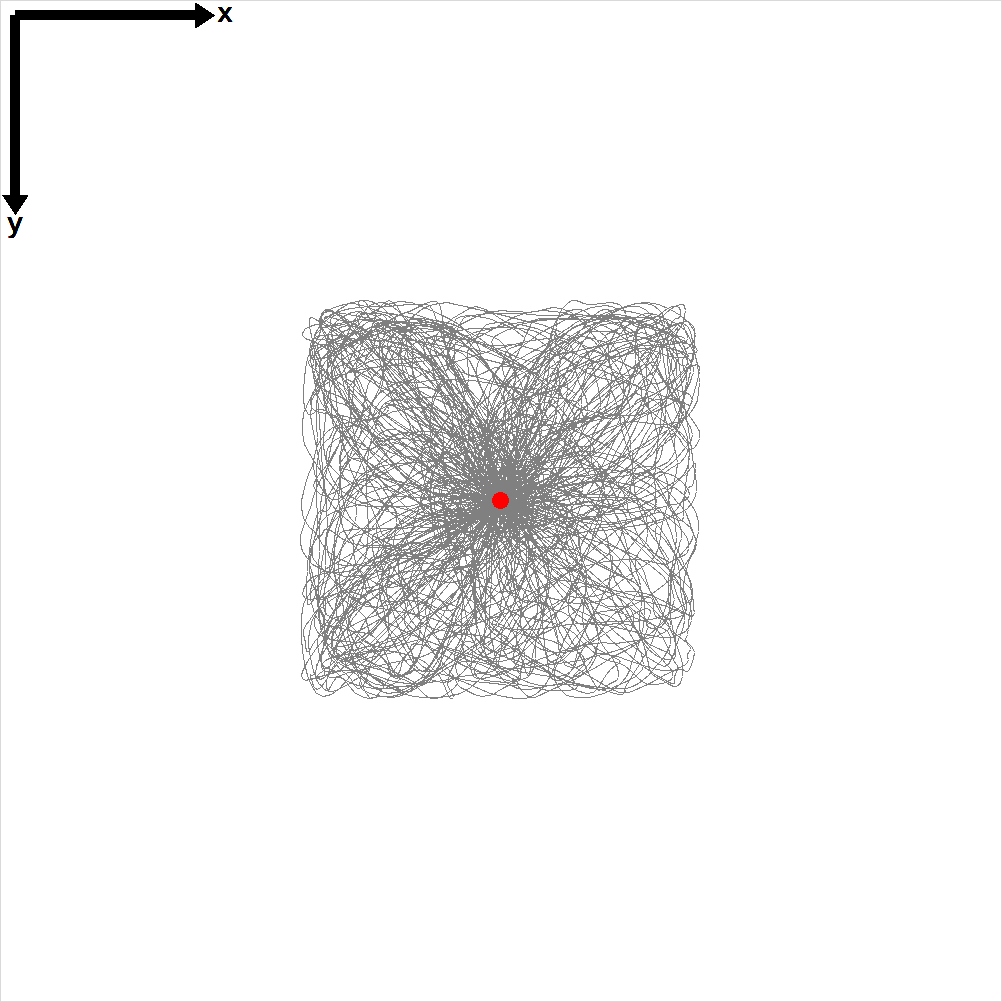
\includegraphics[width=.96\linewidth]{diagrams/roadVisualization_G3.png}
    }
    \subcaption{%
        Roads generated by G3
    }
\end{subfigure}

    \medskip
    \caption{%
        Visualization of roads --- Visualizes the segments of all generated roads.
        Each picture covers all points where \(-250<x<250\) and \(-250<y<250\) except for \cref{subfig:roadVisualizationG2} which is shifted to cover all points with \(-125<x<375\).
        The red point marks the origin.
        The points are connected with straight lines instead of interpolating them as they are when starting a simulation.
    }\label{fig:roadVisualization}
\end{figure}
Further it shows that G1 and G2 restrict the segments of the generated roads to be placed in an area of a size \(\SI{200}{\metre}\times\SI{200}{\metre}\) whereas G3 only uses an area of size \(\SI{100}{\metre}\times\SI{100}{\metre}\).
In comparison G0 uses a larger area and distributes its lanes over the available area.\\
To get an impression about the variety of curvatures of the generated roads \cref{fig:roadCurvatureVisualization} shows the roads rotated and translated such a way that the first road center point is in the origin and the second is right below of it.
\begin{figure}
    \centering
    %!TEX root = ../thesis.tex
\setlength{\fboxsep}{0pt}
\begin{subfigure}[c]{.49\linewidth}
    \fbox{
        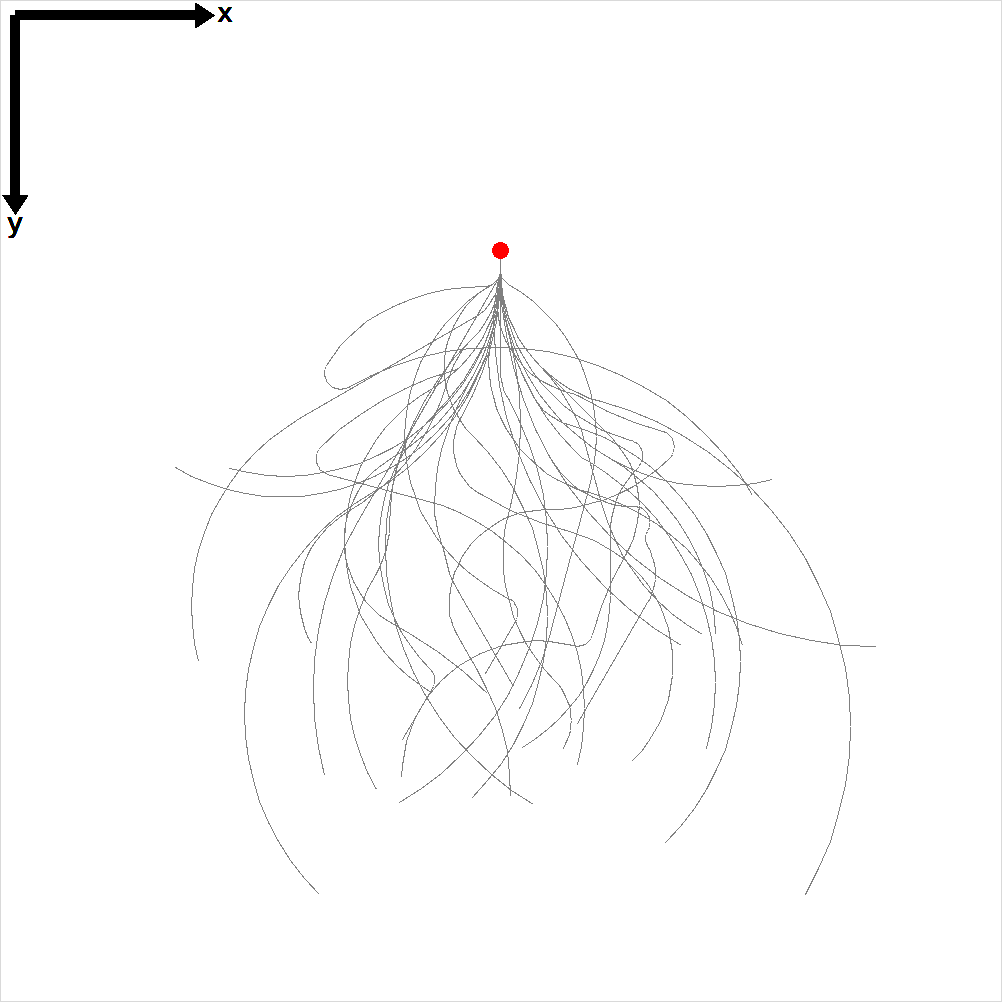
\includegraphics[width=.96\linewidth]{diagrams/roadVisualization_G0_translated.png}
    }
    \subcaption{%
        Curvature of roads generated by G0
    }
\end{subfigure}
\begin{subfigure}[c]{.49\linewidth}
    \fbox{
        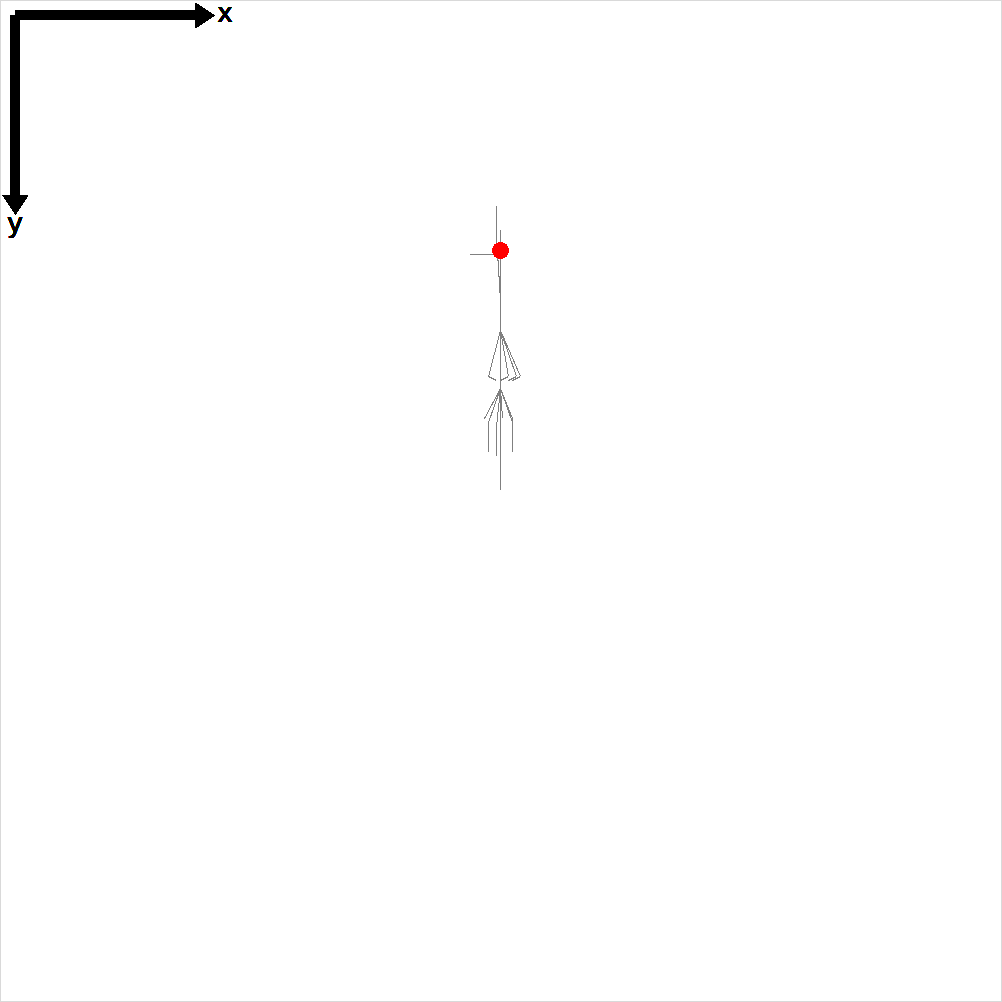
\includegraphics[width=.96\linewidth]{diagrams/roadVisualization_G1_translated.png}
    }
    \subcaption{%
        Curvature of roads generated by G1
    }
\end{subfigure}
\begin{subfigure}[c]{.49\linewidth}
    \fbox{
        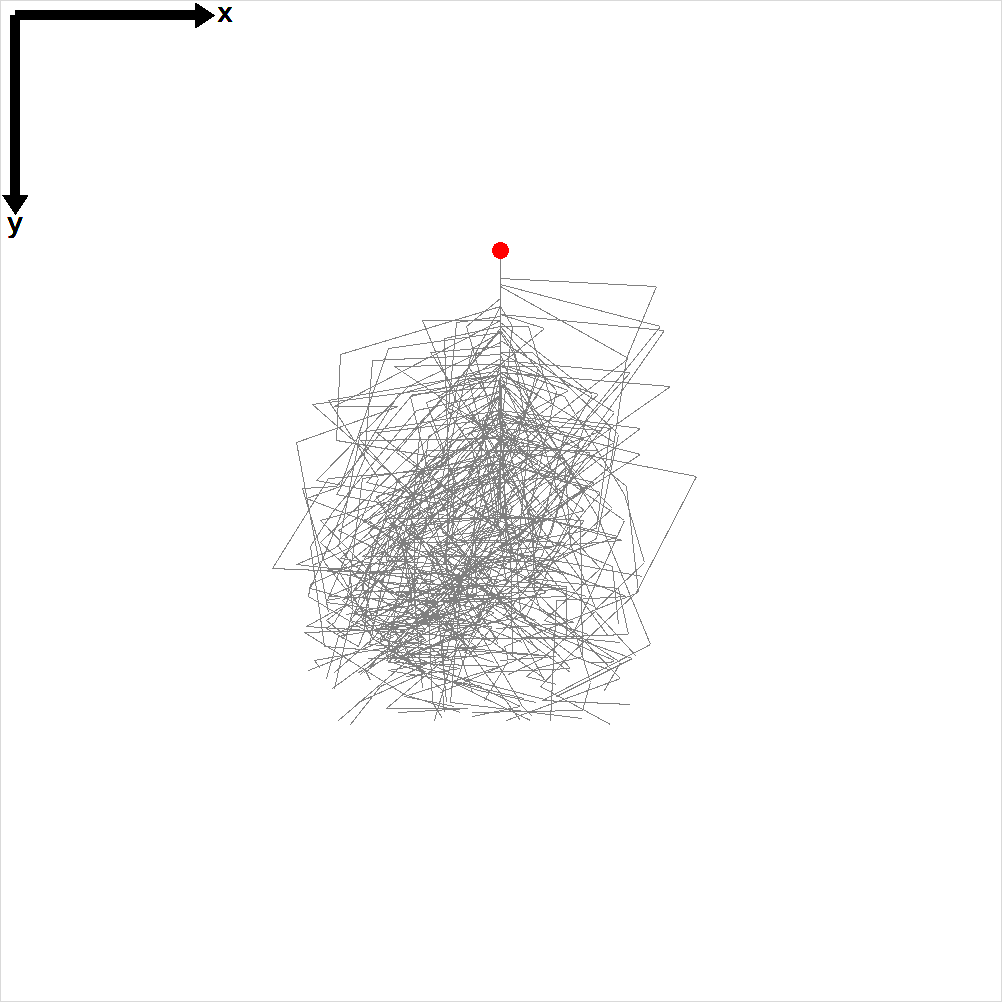
\includegraphics[width=.96\linewidth]{diagrams/roadVisualization_G2_translated.png}
    }
    \subcaption{%
        Curvature of roads generated by G2
    }
\end{subfigure}
\begin{subfigure}[c]{.49\linewidth}
    \fbox{
        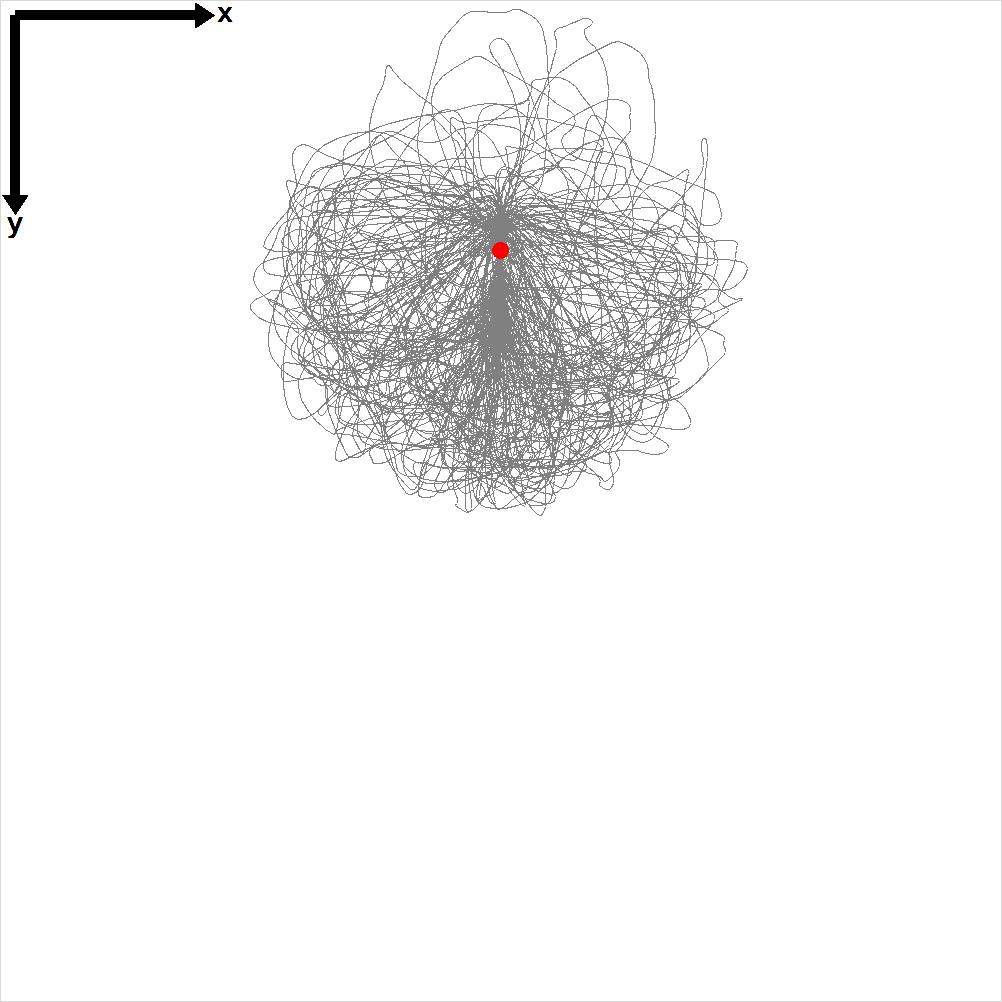
\includegraphics[width=.96\linewidth]{diagrams/roadVisualization_G3_translated.png}
    }
    \subcaption{%
        Curvature of roads generated by G3
    }
\end{subfigure}

    \medskip
    \caption{%
        Visualization of road curvatures --- Visualizes the segments of all generated roads but equally rotated based on the first two road segments and translated to start at the origin.
        Each picture covers all points where \(-250<x<250\) and \(-125<y<375\).
        The red point marks the origin.
    }\label{fig:roadCurvatureVisualization}
\end{figure}
The roads generated by G0 consist mainly of one or two big curves and often face in a similar direction.
Only occasionally a road has multiple curves that head in different directions and it rarely has sharp turns or long straight sections.
G1 generates solely almost short and straight roads as expected from \gls{ac3r}.
The center points of the roads generated by G2 seem to be uniformly and randomly distributed over a predefined area which contradicts with its claim to use \asfault{} for the generation.
G3 generates highly diverse and complex roads with many curves having different directions and sizes.
The generated roads may even revolve the initial position which makes the roads interesting on an intuitive level.
To estimate how interesting the generated roads are future work may use quantitative metrics~\cite{generationForRacingGames} to further investigate the generated roads.\\
\Cref{fig:traveledDistancesVisualization} visualizes how far \glspl{av} traveled on generated roads.
\begin{figure}
    \centering
    %!TEX root = ../thesis.tex
\setlength{\fboxsep}{0pt}
\begin{subfigure}[c]{.49\linewidth}
    \fbox{
        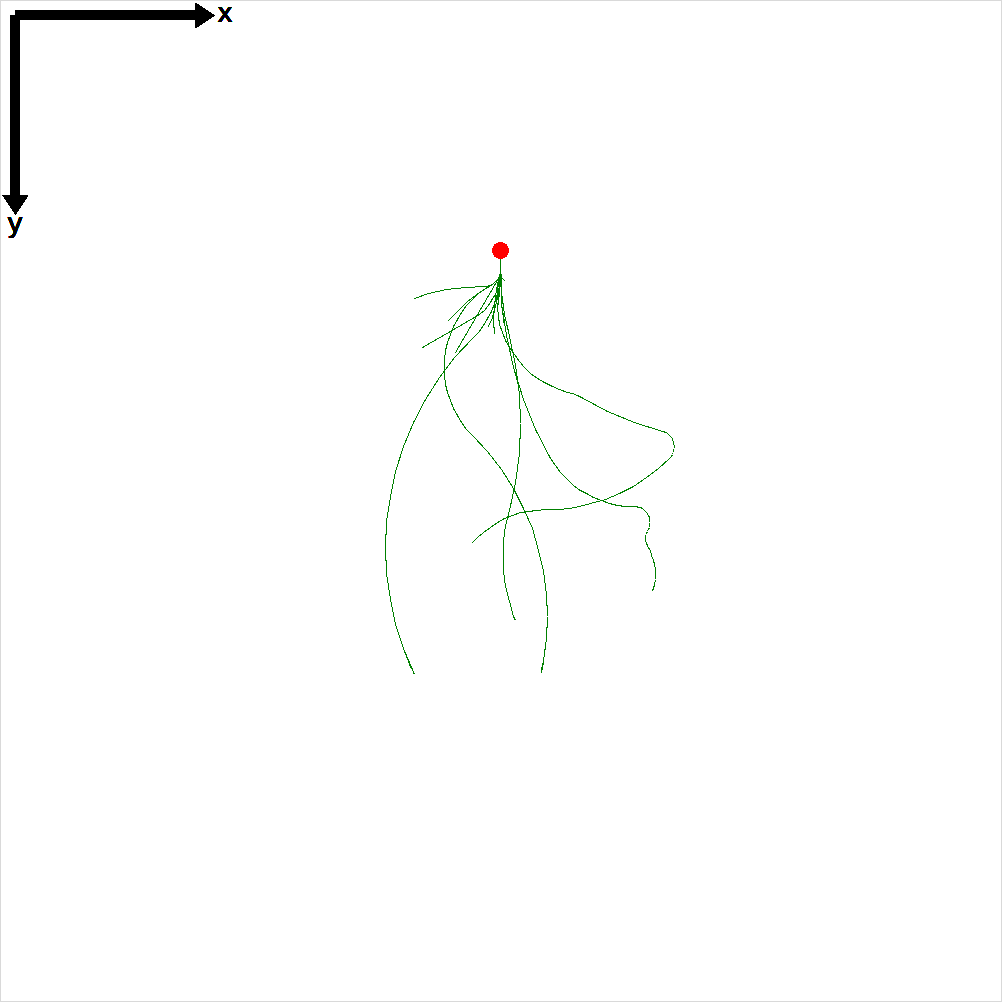
\includegraphics[width=.96\linewidth]{diagrams/roadVisualization_G0_traveled.png}
    }
    \subcaption{%
        Traveled distances on roads generated by G0
    }
\end{subfigure}
\begin{subfigure}[c]{.49\linewidth}
    \fbox{
        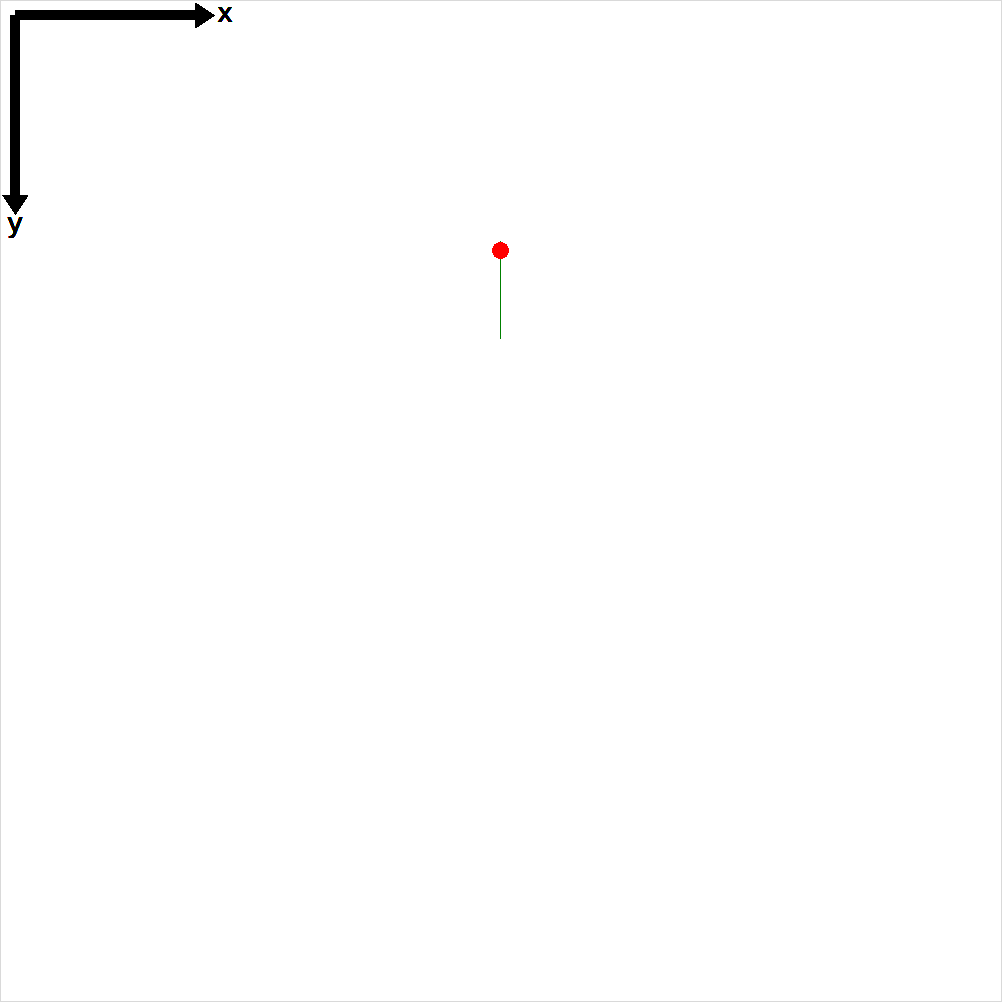
\includegraphics[width=.96\linewidth]{diagrams/roadVisualization_G1_traveled.png}
    }
    \subcaption{%
        Traveled distances on roads generated by G1
    }
\end{subfigure}
\begin{subfigure}[c]{.49\linewidth}
    \fbox{
        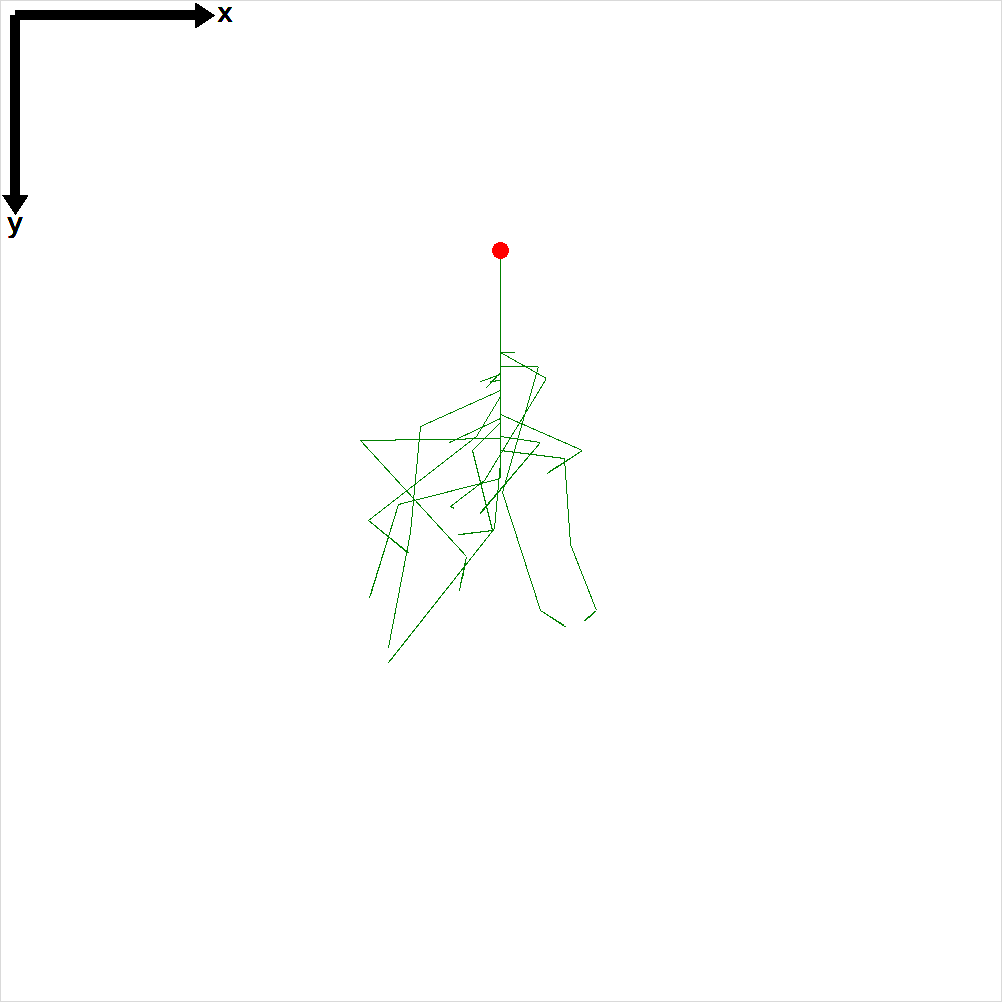
\includegraphics[width=.96\linewidth]{diagrams/roadVisualization_G2_traveled.png}
    }
    \subcaption{%
        Traveled distances on roads generated by G2
    }
\end{subfigure}
\begin{subfigure}[c]{.49\linewidth}
    \fbox{
        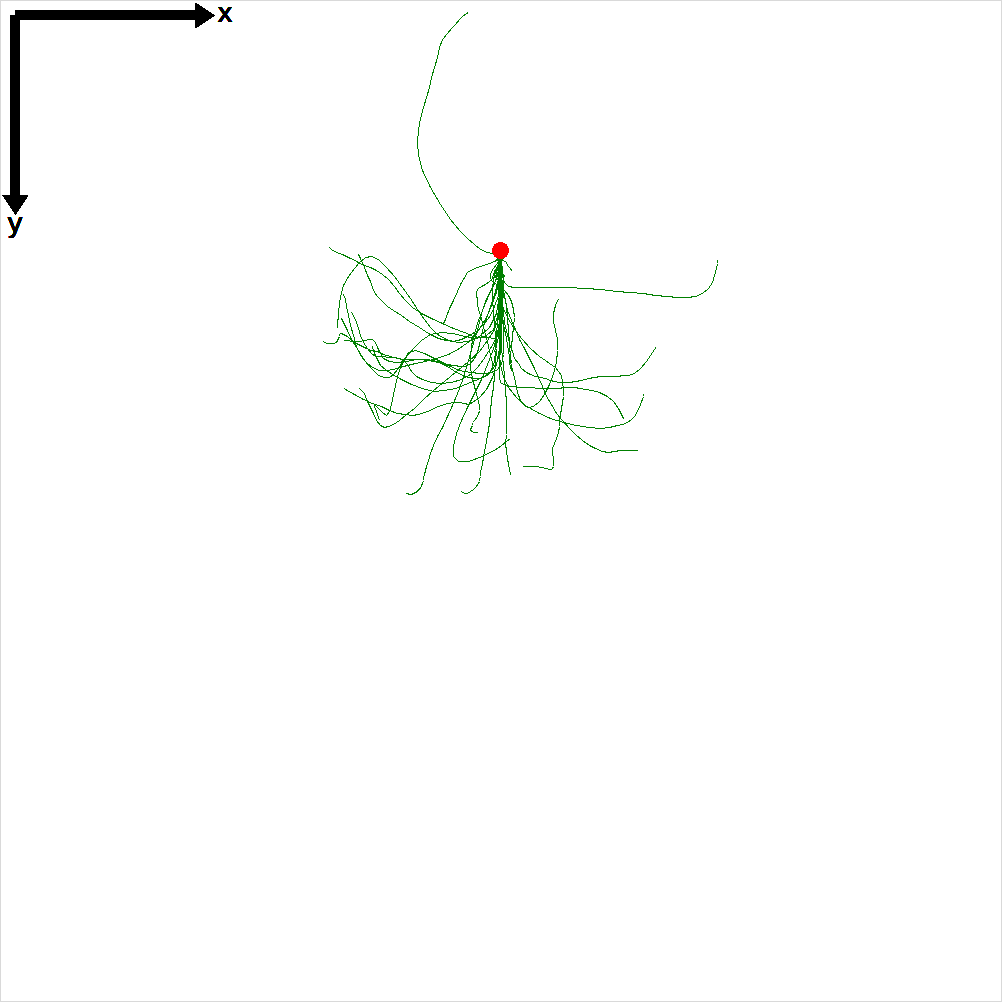
\includegraphics[width=.96\linewidth]{diagrams/roadVisualization_G3_traveled.png}
    }
    \subcaption{%
        Traveled distances on roads generated by G3
    }
\end{subfigure}

    \medskip
    \caption{%
        Visualization of traveled distances --- Visualizes the segments of all roads in \cref{fig:roadCurvatureVisualization} but depicts only the actually traveled segments.
        Each picture covers all points where \(-250<x<250\) and \(-125<y<375\).
        The red point marks the origin.
    }\label{fig:traveledDistancesVisualization}
\end{figure}
Comparing \cref{fig:traveledDistancesVisualization} with \cref{fig:roadCurvatureVisualization} shows that the ratio of the distance \glspl{av} under test traveled to the length of the roads is low.
This confirms that either the \glspl{ai} have no good lane keeping capabilities except for A0 which has perfect knowledge about the lanes or the test generators are very effective in finding bugs in the lane keeping capabilities of \glspl{ai}.
\subsubsection{Effectiveness of Test Generators}
The effectiveness estimates how effectively a test generator can find bugs in \glspl{ai}.
The effectiveness of test generators is computed by dividing the number of failed tests through the sum of failed and successful tests.
The \num{8} executions of the challenge test yielded in total \num{1208} generated tests where \num{1114} were valid and could be executed.
\Cref{fig:numTestsPerGenerator, fig:numTestsPerAI} show all test results and group them by either the test generator or the \gls{ai}.
\begin{figure}
    \includesvg[width=\textwidth]{diagrams/diagram12a.svg}
    \medskip
    \caption{%
        Test results --- Depicts the number of generated tests and groups them by test generator.
        It further distinguishes the number of generated tests based on their test result where \code{ERRORED} and \code{NOT MOVING} are no actual test results but denote that the test generator failed to generate a test or the connected \gls{ai} did not move respectively.
    }\label{fig:numTestsPerGenerator}
\end{figure}
\begin{figure}
    \includesvg[width=\textwidth]{diagrams/diagram12c.svg}
    \medskip
    \caption{%
        Test results --- Divides the executed tests by their result and groups them by the connected \gls{ai}.
        The test results \code{NOT MOVING} and \code{ERRORED} are no actual test results but denote that an \gls{ai} did not move or its implementation threw an error.
    }\label{fig:numTestsPerAI}
\end{figure}
The computation of the effectiveness considers only successful and failed tests but there are more tests.
According to \cref{fig:numTestsPerGenerator} G0 and G1 \gls{av} did not move in some tests.
An \gls{av} is considered as non moving if it does not move more than \SI{5}{\metre} within the first \SI{60}{\second} of the simulation.
These two values are chosen based on a sophisticated guess considering the startup time of \beamng{} and the possible computation overhead of the connected \gls{ai}.
Since according to \cref{fig:numTestsPerAI} the only \gls{ai} that did not move in some tests cases is A0 it is very likely that G0 and G1 did not always define goal positions that fulfill all restrictions inherited by the \beamng{} \gls{ai}.
Additionally many generations of G1 resulted in an error.
According to the log of the challenge executions errors occur because the download of a police report fails, \gls{ac3r} throws an error or \gls{ac3r} is not able to translate the police report into a comprehensive simulation.
In addition many tests result in a timeout which means that a test does neither fail nor succeed within a predefined time.
This can happen if the connected \gls{ai} does not respond \ie{} continue with the execution of the client scheme or the success criterion is either infeasible or the \gls{ai} requires more knowledge about the scenario to fulfill it \eg{} a goal area which is behind but not in front of the \gls{av}.
This timeout consideration applies also for G3.\\
\Cref{tab:effectivenessGenerators} lists how many of the executed tests succeeded and failed per test generator as well as the resulting effectiveness.
\begin{table}
    \centering
    \caption{%
        Test generator effectiveness --- Displays the calculation of the effectiveness of the test generators.
        Higher values indicate higher effectiveness.
    }\label{tab:effectivenessGenerators}
    \medskip
    \begin{tabularx}{.5\linewidth}{X c c c c}
    \toprule
    \bfseries Property & \bfseries G0 & \bfseries G1 & \bfseries G2 & \bfseries G3 \\
    \midrule
    \#Failed      & \num{161}  & \num{117}  & \num{200}  & \num{198}  \\
    \#Succeeded   & \num{32}   & \num{36}   & \num{229}  & \num{73}   \\
    Sum           & \num{193}  & \num{153}  & \num{429}  & \num{271}  \\
    Effectiveness & \num{0.83} & \num{0.76} & \num{0.47} & \num{0.73} \\
    \bottomrule
\end{tabularx}

\end{table}
Compared to the other generators G2 is less effective in generating tests that trigger faulty behavior of \glspl{ai} although it should be very similar to G0.
Both generate always exactly one participant which drives on a single road and both claim to use \asfault{} for generating roads.
G2 has in contrast to G0 very small roads and additionally adds obstacles to its test scenarios (see \cref{fig:numElements}).
So one would expect G2 to be more effective than G0 since it should be more likely that an \gls{av} goes off-road or crash into an obstacle. 
This is clearly not the case.
G0, G1 and G3 have a high effectiveness which mainly results from the bad lane capabilities of the \glspl{ai} that the short traveled distances (see \cref{fig:traveledDistancesVisualization}) suggest.\\
According to \cref{fig:numElements} G1 is the only generator that adds more than one participant and one road.
Since the \glspl{ai} focus on lane keeping and not on crash avoidance the test generators reveals many bugs and therefore it has a high effectiveness.
\Cref{fig:goalRegionSizes} shows the area sizes of the goal regions (in \si{\metre^2}) the test generators defined for the \gls{av} under test to reach.
\begin{figure}
    \includesvg[width=\textwidth]{diagrams/diagram13a.svg}
    \medskip
    \caption{%
        Goal area sizes --- Shows the sizes of generated goal areas that vehicles have to reach in order to succeed a test.
        It only considers valid goal definitions of goal regions.
    }\label{fig:goalRegionSizes}
\end{figure}
The area of the goal regions G0 generates is constant.
To define the goal region in a test G0 selects the road center point of the last segment of the generated road and specifies at this point a goal position having a tolerance radius identical to the width of the road.
Since the width was fixed during the challenge test the size of the resulting goal regions is constant.
In a similar way G3 chooses one of the road center points and defines the goal region by a square with a fixed edge length of \SI{20}{\metre} around the point.
So the size of the resulting goal areas is constant as well.
G1 generates the smallest goal areas which results from the fact that the generated tests are very compact and do not require big goal areas.
G2 generates vastly bigger goal areas which are likely to contain almost the whole environment.
A look into the implementation of G2 reveals that it uses the first and the last two road center points to create a huge triangle which then defines the goal region of a test.
Hence often an \gls{av} almost immediately succeeds a test without driving at all which leads to the low effectiveness of G2.
\Cref{fig:executionTimesAIs} depicts for how long \glspl{ai} drove in simulations of generated tests and supports this observation.
\begin{figure}
    \includesvg[width=\textwidth]{diagrams/diagram14a.svg}
    \medskip
    \caption{%
        Execution times of \glspl{ai} --- Visualizes the time that \glspl{ai} drove on tests scenarios until the simulation finished without being canceled and without timeout.
    }\label{fig:executionTimesAIs}
\end{figure}

\subsection{Evaluation of Scalability}\label{subsec:evaluationOfScalability}
This experiment is organized in two parts.
The first part evaluates the scalability of a single \gls{simnode} which runs on real hardware.
The second part examines whether \glspl{simnode} can be hosted by \glspl{vm}, whether this influences the results of executed tests and the benefits of distributing simulations across multiple \glspl{simnode}.
For the experiment I used a fixed test scenario \(T\) which was generated by G0.
\(T\) defines a single road and places a single \gls{av} on it that has to follow the road to succeed the test.
To control the \gls{av} I used A0 (see \cref{subsubsec:submissions}) and \(T\) is configured to request it every \SI{0.5}{\second}.
The timeout for test executions is fixed to \SI{10}{\minute}.\\
The first part of the experiment used a setup of \drivebuild{} where node~2 (see \cref{tab:nodeSpecifications}) was the only connected \gls{simnode}.
In each round I created between \num{1} and \num{10} instances of \(T\) and submitted them to \drivebuild{} all at once.
\Cref{fig:scalabilityCompleteExecutionTimesLaptop} shows the execution time for each of the \num{10} rounds.
\begin{figure}
    \includesvg[width=\textwidth]{diagrams/diagram20a.svg}
    \medskip
    \caption{%
        Execution times --- Shows the scalability of \drivebuild{} based on the number of tests submitted at once.
        It also shows a linear regression line (blue) and the linear projection if the instances of \(T\) were executed sequentially (red).
    }\label{fig:scalabilityCompleteExecutionTimesLaptop}
\end{figure}
Every execution of \(T\) in every round succeeded except for one execution in round~9 which yielded a timeout.
When submitting \num{9} or more instances of \(T\) at once the simulations get so slow that some of them may exceed the timeout and thus not succeed as they would if they were less simultaneously running instances of \(T\).
To avoid this problem each \gls{simnode} defines a maximum number of simulations it can handle simultaneously.
If every \gls{simnode} reached the limit \gls{http} requests for submitting more tests \drivebuild{} rejects them stating that there were too many active requests.
For sake of this experiment I disabled this limit on every \gls{simnode}.
However, the diagram clearly visualizes that \drivebuild{} is able to utilize parallelism to speedup test executions as this work claimed.
Further the regression line suggests that the execution time for less than \num{11} tests is linear.
But much more test executions with even more instances of \(T\) are required to support this observation.\\
\Cref{fig:scalabilityExecutionTimesLaptop} shows how long the execution of each single instance of \(T\) in any round took to complete.
\begin{figure}
    \includesvg[width=\textwidth]{diagrams/diagram19b.svg}
    \medskip
    \caption{%
        Test executions --- Visualizes when tests started and how it took until they ended.
        It visualizes succeeded tests as well as tests which yielded a timeout.
        The diagram also includes a vertical line which marks the configured timeout.
    }\label{fig:scalabilityExecutionTimesLaptop}
\end{figure}
It also visualizes when executions of \(T\) started and how they took until they ended.
The relative start of the tests per round reveals that the startup time of \beamng{} is about \SI{50}{\second}.
According to \cref{fig:scalabilityCompleteExecutionTimesLaptop} the execution of a single instance of \(T\) takes about \SI{210}{\second}.
Hence the startup of \beamng{} takes almost a quarter of the complete execution time of a single instance.
The diagram also shows that the earlier a test in a round is started the longer it takes to complete and tests in the same round often complete almost at the same although they start offset and each test should take the same time.
One possible explanation might be that \drivebuild{} has a bug which \eg{} makes test executions synchronize with each other and finish at the same time.
I was not able to verify such a bug through manual test executions.
\drivebuild{} does not implement any explicit prioritization of messages.
Hence, another possible explanation might be that the message exchange of \drivebuild{} assigns higher priorities to certain messages implicitly.
A \gls{simnode} maintains one socket the \gls{mainapp} uses to start an instance of \(T\) and additionally maintains two open sockets for each running instance of \(T\).
One socket accepts commands for the \gls{av} which the client sends over the \gls{mainapp}.
This socket yields \code{waitForSimulatorRequest} and \code{requestData} (see \cref{tab:simNodeToMainAppInterface}) alternately.
The other socket accepts commands from the runtime verification.
Having this in mind one possible scenario which might lead to the observed results is that starting new tests has implicitly a higher priority than commands from runtime verification cycles \eg{} stop a simulation when it succeeded or timed out.
To validate these explanations further investigation is required.\\
The second part of the experiment used a setup with either \num{1}, \num{2} or \num{3} \gls{simnode}\unskip{}s which were installed on \glspl{vm} (see node~3 in \cref{tab:nodeSpecifications}).
The \glspl{vm} are managed using the \gls{slurm}~\cite{slurm}.
Since \beamng{} is only available for Windows every \gls{vm} has to run Windows.
Further \beamng{} requires a good \gls{cpu} as well as a very good \gls{gpu}.
To minimize the expected performance loss \gls{slurm} provides direct and isolated access to the \gls{gpu}.
So the \gls{gpu} is not shared with any other program running on a \gls{slurm} node.
I create either \num{1}, \num{2}, \num{5} or \num{8} instances of \(T\) and submit them to \drivebuild{} at once which yields a total of \num{12} executions of the experiment with different configurations.
Since it took over a week to collect the data for the second part I did not repeat the experiment.
In contrast to the results of the first part the test executions result in many timeouts as \cref{fig:scalabilityResults} depicts.
\begin{figure}
    \includesvg[width=\textwidth]{diagrams/diagram18a.svg}
    \medskip
    \caption{%
        Scalability results for \glspl{vm} --- Shows how many tests finished depending on the number of available \glspl{simnode} and the number of submitted tests.
        The higher the values the more reliable are test executions on \glspl{vm}.
    }\label{fig:scalabilityResults}
\end{figure}
This results from the very poor performance of \beamng{} when executed on a \gls{vm}.
On the one hand, the diagram shows that an increasing number of simultaneously submitted tests rapidly decreases the percentage of tests that properly finish.
On the other hand, the diagram does not indicate that a higher number of \glspl{simnode} increases the percentage of properly finished tests.
Concerning the executions of the experiment which submitted \num{8} tests at once \num{3} tests finished with \num{2} \glspl{simnode} connected, only \num{2} finished with a single \gls{simnode} connected whereas only \num{1} test finished with \num{3} \glspl{simnode} connected.
This observation may result from the fact that the \gls{slurm} cluster which hosts the \glspl{simnode} is shared with other researchers and thus it is used intensively and under heavy but varying load.
The observation may be also a result of the low reliability of the low level socket communication between the \gls{mainapp} and the \glspl{simnode}.
If a socket is not used for a certain time interval it closes its connection which leads to a timeout of the simulation the socket has to handle messages for.
To investigate these problems in more detail much more test executions with \glspl{simnode} that are not hosted in \glspl{vm} are required.

\subsection{Experience Report}\label{subsec:experienceReport}
\subsubsection{Process}
The creation of a test generator or an \gls{ai} is not trivial and requires a good understanding of the concepts to apply.
Additionally when it comes to trying out the implementations the students had to deal with many new technologies which are involved in creating the program including libraries, frameworks, development tools as well as to set up a simulator, handle simulations and collect data.
To avoid the problems concerning the actual simulations and retrieving data I encouraged students to try out their implementations using \drivebuild{}.
To enable them to use \drivebuild{} I presented them the basic strategies and concepts \drivebuild{} implements and showed them short code examples of possible test definitions \ie{} \gls{dbc} and \gls{dbe} \gls{xml} files as well as a basic \gls{ai} implementation.
I did neither explain the implementation nor the underlying communication protocol to the students.
Instead I provided them a client \gls{api} which hides the details of the \gls{http} based communication.
I suggested students to use debuggers to get to know how the requested data and the abstract data objects look like.
I have been available for them to request help during the implementation of their programs, to request features which address their needs and to provide feedback for \drivebuild{}.
I implemented feature requests like an additional data request for requesting the heading angle and the automatic creation of road markings.
I did not implement all of their features requests \eg{} weather conditions.
The future work section mentions some of the feature requests which are not implemented yet.
\subsubsection{Experience}
Concerning the fact that the seminar targets master students and bachelor students in higher semesters the level of skill and knowledge of some students was unexpectedly low.
The \gls{xsd} provided with \drivebuild{} is very long and uses advanced mechanisms including abstract elements and substitution groups and some tried to fully understand it.
Some students never heard of \gls{xml}, never used it and had no idea how to validate \gls{xml} against \gls{xsd}.
Hence there was no chance for them to get an overview over the whole range of capabilities the test formalization offers.
Instead I showed them only the most basic features such as the definition of roads, the placement of participants plus the usage of the two criteria for damage and off-road detection.
Many students struggled to use predefined Python libraries which for example provide a tensorflow implementation that they require for their \gls{ai} implementation.\\
For the students that implemented test generators one of the most complex topics was \gls{xml} and its validation with \gls{xsd}.
Many of them used the example definitions I provided almost literally and only selectively modified them.
When they tried to introduce the damage and off-road oracles some of them failed since they did not understand how to use logical operators to create compound conditions like \enquote{A test fails if an \gls{av} is damaged \underline{or} is off-road}.
No one of the students used more than a single connective and no student utilized any kind of nested criteria because this requires at least an intuitive understanding of temporal logic.\\
The most complex topics for the students implementing \glspl{ai} were the necessary understanding of the runtime verification cycle and the client scheme plus how these interact with each other.
Some students struggled to get an intuitive understanding of parallelism, why it is needed to control multiple \glspl{av} at once and to handle parallel threads with \code{start} and \code{join} calls.
It was further difficult to explain them what data \glspl{ai} can request, how to declare it for an \gls{av} and what the data response looks like.\\
Some of the students did not succeed to either create something which runs on its own and utilizes \beamng{} or to create at least something which can be integrated with \drivebuild{}.
The integration of the submissions was difficult because many students did not provide a comprehensive list of requirements.
Further there are restrictions to minimum and maximum versions of packages, frameworks and Python itself.
Especially setting up and integrating \gls{ai} implementations was very time consuming since these implementations rely on multiple complex libraries.
\Glspl{ai} additionally have external dependencies and some of the requirements and dependencies conflicted.
Hence the list of dependencies the \submissiontester{} requires is long (see \cref{tab:stUsedTools}).
Another problem with \glspl{ai} is to properly choose values for configuration parameters like initial population sizes since students did not document them.
Further the implementation of the interface of \glspl{ai} is not only required to use the predefined signature but also to implement the client scheme shown in \cref{fig:clientScheme}.\\
Multiple students did not or at least not properly implement the interface for the \submissiontester{} as described in \cref{fig:testGeneratorStub,fig:aiStub}.
So I had to create, fix and extend most of the interfaces the students provided to me.
To make sure executions of submissions do not interfere with each other the \submissiontester{} has to separate them.
Most of the submissions use paths relative to the current working directory instead of relative to the called file.
Thus I also had to change all hard coded paths to make submissions work.
Some submissions had bugs resulting from an insufficient understanding of the concepts students should implement.
To fix them I was required to have a deep understanding of the strategies the students targeted to implement them myself.\\
The gained experience reveals that there are aspects which could be done or handled differently in future work.
One problem is the potentially conflicting dependencies and requirements the submissions of the students introduce to the \submissiontester{}.
To avoid these conflicts the \submissiontester{} could use separate Python environments for each submission.
As a drawback this requires to create and maintain multiple Python environments and to activate and deactivate them dynamically.
This also increases the complexity of interacting with submissions and most presumably requires students to implement more complex interfaces.
Another approach would be to use \docker{}~\cite{docker}.
Additionally to the advantages like when having multiple Python environments \docker{} enables to start submissions in a clean state and to start multiple instances of the submissions.
At the current point it is not clear whether these features are required.
The approach also shares the same drawbacks but in a higher form since the effort of creating and maintaining docker containers which include Python environments is higher than maintaining Python environments directly.
Further the activation and deactivation as well as the interaction with \docker{} containers is even more complex and most presumably requires students to implement even more complex interfaces.
The interfaces for the \submissiontester{} currently pass test case definitions as paths to files containing \gls{xml}.
Since the test case definitions have to be modified for the evaluation it would be easier to deal with \gls{xml} trees directly instead of file paths.
The evaluation shows that the reliability of the low level socket communication might be a problem especially when hosting \glspl{simnode} in \glspl{vm} and should be improved.
Another thread to the reliability is \beamngpy{} since it is not designed to cope with parallel requests to the same \beamng{} instance.\\

    %!TEX root = ../thesis.tex
\section{Conclusions}
% Based on https://www.scribbr.com/dissertation/write-conclusion/
In this work I developed a distributed system which automates simulation-based testing of \glspl{av}.
Therefore it presents a formalization of test cases and explains all relevant strategies to generate simulations, handle simulator instances, evaluate test criteria during simulation executions, distribute simulation executions over a cluster and implement the communication between the components of \drivebuild{} and clients.
Its evaluation works with students as users of \drivebuild{} and utilizes their implementations of test generators and \glspl{ai}.
It showed that \drivebuild{} is able to cope with all these various approaches.
Further \drivebuild{} provides all metrics that either the implementations require to operate or the evaluation requires to analyze them.
Since the number of available test generators and \glspl{ai} is low and the quality of some of them is not as good as expected the metrics to analyze them yielded not as much interesting information as they could.
So future evaluation should consider even more test generators and \glspl{ai} (\eg{} \gls{dave}~\cite{dave}).
The evaluation also illustrates that \drivebuild{} is able to distribute test executions among a cluster and handle simulations and \glspl{av} in parallel.
Further it reveals that the performance when running \glspl{simnode} in \glspl{vm} on a shared cluster is very bad.
Research on the causes that affect the performance issues requires much more test executions and dedicated hardware resources.
Based on the experience which the evaluation yields possible causes may be low reliability of the low level socket communication or the fact that the hardware is virtualized.\\
However, there are already seminar courses at the university of Passau which use \drivebuild{} to test \glspl{ai}.
Further there is an ongoing discussion with researchers at the \enquote{Université du Québec à Chicoutimi, Canada} about integrating their event stream processing into \drivebuild{} to implement runtime verification and real-time monitoring.
Also at the \gls{zhaw} there is a thesis about testing \glspl{av} which utilizes \drivebuild{}.

    %!TEX root = ../thesis.tex
\section{Future Work}
\drivebuild{} does not provide any visual feedback that shows more than camera images of participants.
Visual feedback is very important to get feedback about the generated environments and to get an intuitive understanding of the movement of \glspl{av}.
For the visualization a format like \gls{rosbag}~\cite{rosbag} could be introduced.
\Gls{rosbag} is a format which stores sequences of pixel clouds to represent a simulation.
This allows to visually debug simulations in 3D and rewind a simulation forward and backward.
Already a simple visual representation (\eg{} a bird view like screenshot) of the environment as well as the initial states, positions and orientations of participants in this environment might be interesting for testers to get an idea about the setup of a test before it is executed.
There is already an ongoing project which plans to extend \drivebuild{} with a debugger which visualizes the simulation and allows to define breakpoints, to pause and resume simulations plus to dynamically evaluate expressions during a simulation.\\
Concerning the initial orientation of participants \drivebuild{} defines angles relative to the ground.
The experience of this work shows that for test generators it would be easier to specify the initial orientation of participants relative to the underlying road instead of the ground.\\
To determine whether an \gls{av} is off-road, drives on a certain road or is within a certain region \drivebuild{} uses either the bounding box or the center position of the \gls{av}.
In order to cooperate with \beepbeep{}~\cite{beepbeep} future work should formalize these checks more precisely.\\
The load balancing of \drivebuild{} considers only the number of currently running tests on any \gls{simnode}.
A prediction of the resulting load of a simulation based on characteristics of submitted \glspl{dbe} and \glspl{dbc} may improve the load balancing.
To further improve the load balancing certain messages like \enquote{stop} may have a higher priority whereas messages that start new simulations may have a lower priority.
The priority of messages may be also dependent on the estimated remaining execution time of running simulations or their progress.\\
Currently \drivebuild{} is only able to generate road markings for single roads which do not change their width and the number of lanes.
Future work may improve road markings by considering junctions, varying number of lanes, variable road width and more types of road markings including broken or dirty road markings.\\
A future version of \drivebuild{} may be able to set different weather conditions including rain, snow and slippery roads to check whether and compare how well \glspl{av} can cope with it.\\
\drivebuild{} provides training data in terms of traces (see \cref{fig:databaseScheme}).
To provide even more training data future work may introduce additional approaches like \scenic{} which uses the previously collected data to generate even further new data.
Training data may also include the reasons why tests failed or succeeded.
Therefore it is required to detect in case the failure or success criterion was triggered which elements of the representing temporal logic expression were involved to fulfill the criterion.\\
In future versions \drivebuild{} may also ship with a predefined set of test generators and \glspl{ai}.
Therefore it may be interesting to allow a test setup for an \gls{ai} to specify restrictions on the generated roads like disallowing self intersection of roads.

    \pagebreak

    \section{Acronyms}
    \begingroup
    \renewcommand{\section}[2]{}
    \printglossary[type=\acronymtype, style=mcolindex]
    % \glsaddallunused[\acronymtype] % FIXME Do not show unused acronyms
    \endgroup
    \pagebreak

    \section{References}
    \begingroup
    \renewcommand{\section}[2]{}
    \printbibliography[category=cited]
    \endgroup

    % \section{Not cited} % FIXME Do not show not cited references
    % \begingroup
    % \renewcommand{\section}[2]{}
    % \printbibliography[notcategory=cited]
    % \endgroup

    \pagebreak
    \appendix
    %!TEX root = ../thesis.tex
\section{Appendix}
\FloatBarrier%
\subsection{Code Example Snippets}
\begin{figure}[h]
    \captionsetup{type=listing}
    \inputminted{xml}{code/exampleEnvironment.dbe.xml}
    \medskip
    \caption{%
        Example environment description --- This example shows a basic environment description defining two roads.
        \Cref{fig:exampleEnvironmentVis} shows the resulting generated roads.
    }\label{fig:exampleEnvironment}
\end{figure}
\begin{figure}[h]
    \captionsetup{type=listing}
    \inputminted{xml}{code/exampleMovement.dbc.xml}
    \medskip
    \caption{%
        Example participant description --- This example shows an example of positioning a participant, defining its movement and which data its \gls{ai} requires.
    }\label{fig:exampleParticipant}
\end{figure}
\begin{figure}[h]
    \captionsetup{type=listing}
    \inputminted{xml}{code/exampleObstacleDefinitions.xml}
    \medskip
    \caption{%
        Example obstacle definitions --- This snippet demonstrates the creation of all available types of static obstacles.
        \Cref{fig:exampleEnvironmentVis} shows a visualization of generated obstacles.
    }\label{fig:exampleObstacleDefinitions}
\end{figure}
\begin{figure}[h]
    \captionsetup{type=listing}
    \inputminted{xml}{code/exampleAIDataRequests.xml}
    \medskip
    \caption{%
        Examples for \gls{ai} request data --- This snippet shows all supported types of data that an \gls{av} can request.
    }\label{fig:exampleAIDataRequests}
\end{figure}
\begin{figure}[h]
    \captionsetup{type=listing}
    \inputminted{xml}{code/exampleCriteria.dbc.xml}
    \medskip
    \caption{%
        Example criteria definition --- This snippet shows example definitions for all types of criteria listed in \cref{tab:criteriaTypes}.
        The tag names are built from either the prefix \enquote{vc} or \enquote{sc} and the type name of the criterion.
        To spare duplication the prefix \enquote{x} is used here to denote that the prefix might be either \enquote{vc} or \enquote{sc}.
    }\label{fig:exampleCriteria}
\end{figure}

\FloatBarrier%
\subsection{Determine Target Position for A0}\label{subsec:targetPositionDetermination}
The test generators did not obey the restrictions to the target position that A0 (see \cref{subsubsec:submissions}) introduces.
So in case of A0 the \submissiontester{} has to replace the declared target position with a target position which is valid for A0.
Therefore the \submissiontester{} collects all \code{scPosition} elements within the tag of the success criterion which are associated with the \gls{av}.
If there is exactly one element this defines the target position.
If there are more than one the generated test is considered invalid since the test seems to have a branch in its result.
If there are no \code{scPosition} elements the \submissiontester{} collects all associated \code{scArea} elements within the success criterion that are associated with the \gls{av}.
If there is more than one element the test is again considered invalid since it seems to have a branch in its result.
Only if there is exactly one such element the \submissiontester{} computes the intersection with all roads in the \gls{dbe} and determines all road center points that lie within.
The \submissiontester{} uses one of these points as target position.
If there is no such road center point or there was no associated \code{scArea} the \submissiontester{} uses the last waypoint of the movement which the \gls{dbc} specifies for the \gls{av}.

\FloatBarrier%
\subsection{Used Tools}
% FIXME Including these commands causes problems in the compilation of everything that follows
\LTXtable{\textwidth}{tables/usedTools.tex}
\LTXtable{\textwidth}{tables/stUsedTools.tex}


    \FloatBarrier%
    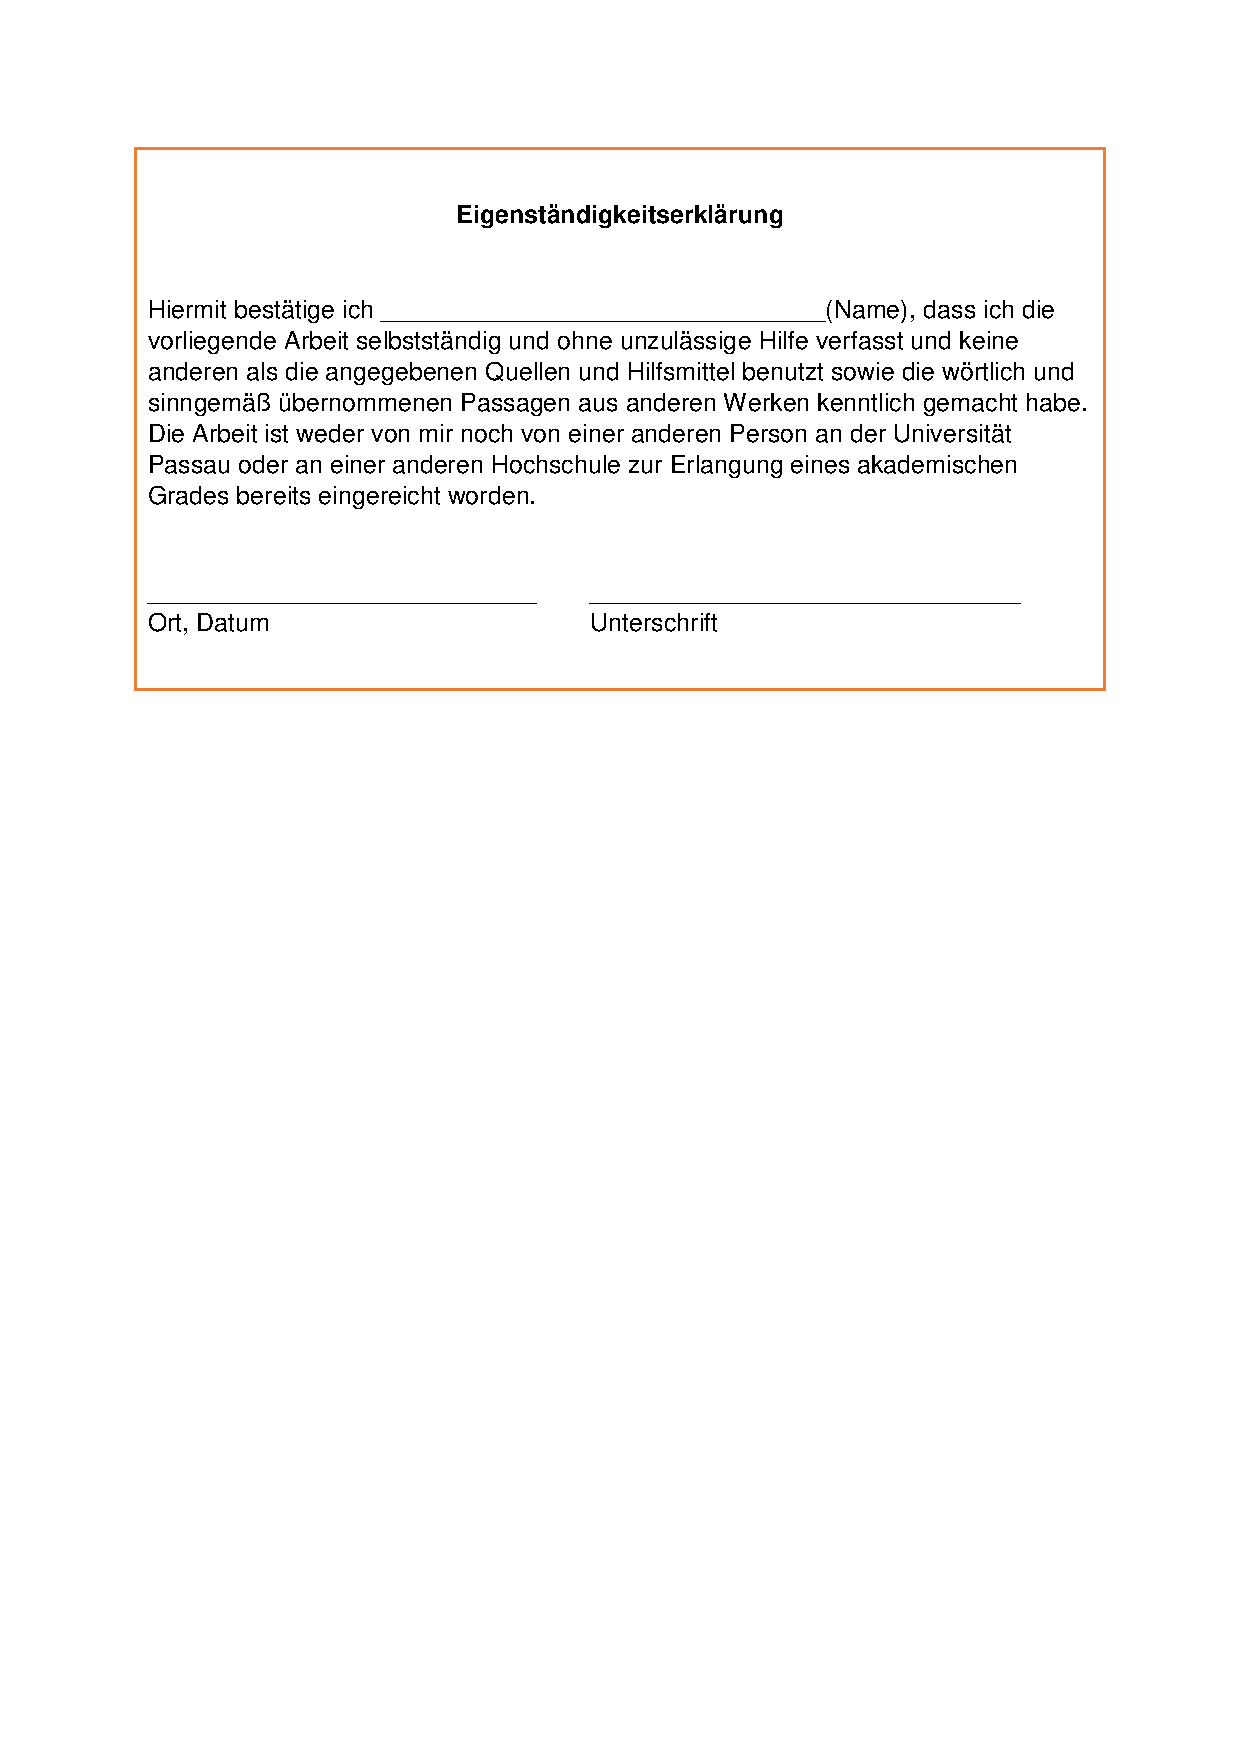
\includepdf[pages=-]{sections/declaration.pdf}
\end{document}
